%%%%%%%%%%%%%%%%%%%%%%%%%%%%%%%%%%%%%%%%%%%%%%%%%%%%%%%%%%%%%%%%%%%%%%%%%%%%%%%%
%                         FORMATO DE TESIS UMSNH                               %
%%%%%%%%%%%%%%%%%%%%%%%%%%%%%%%%%%%%%%%%%%%%%%%%%%%%%%%%%%%%%%%%%%%%%%%%%%%%%%%%
% based on Harish Bhanderi's PhD/MPhil template, then Uni Cambridge
% http://www-h.eng.cam.ac.uk/help/tpl/textprocessing/ThesisStyle/
% corrected and extended in 2007 by Jakob Suckale, then MPI-iCBG PhD programme
% and made available through OpenWetWare.org - the free biology wiki
% forked from https://github.com/Tepexic/Tesis-UNAM on July 2017
% modifications made by Arturo Lopez Pineda

% Modifications made by Elioth Monroy Martos (2018-2019) 

%                     Under GNU License v3

% ADAPTADO PARA UMSNH:  @arturolp

% Adaptado para ESCOM-IPN: @EliothMonroy

\documentclass[oneside,12pt]{Latex/Classes/thesisUMSNH}
%         PUEDEN INCLUIR EN ESTE ESPACIO LOS PAQUETES EXTRA, O BIEN, EN EL ARCHIVO "PhDthesisPSnPDF.cls" EN "./Latex/Classes/"
%\usepackage{blindtext}                        % Para insertar texto dummy, de ejemplo, pues.
\usepackage[square, sort, numbers]{natbib}  % Personalizar la bibliografía a gusto de cada quien
% Note:
%\usepackage{enumerate}
\usepackage{enumitem}
\usepackage{hyperref}
\usepackage{array}
\newcolumntype{P}[1]{>{\centering\arraybackslash}p{#1}}
\newcolumntype{M}[1]{>{\centering\arraybackslash}m{#1}} %Centra tanto vertical como horizontalmente
\newcolumntype{J}[1]{>{\arraybackslash}m{#1}} % Justifica el contenido dentro de una tabla y centra verticalmente
\usepackage{longtable}
\usepackage{graphicx}
\usepackage{verbatim}
\usepackage{listingsutf8}
\usepackage{color}

%Para Times new roman
\usepackage{mathptmx}

\definecolor{codegreen}{rgb}{0,0.6,0}
\definecolor{codegray}{rgb}{0.5,0.5,0.5}
\definecolor{codepurple}{rgb}{0.58,0,0.82}
\definecolor{backcolour}{rgb}{0.95,0.95,0.92}

\lstdefinestyle{mystyle}{
	backgroundcolor=\color{backcolour},   
	commentstyle=\color{codegreen},
	keywordstyle=\color{magenta},
	numberstyle=\tiny\color{codegray},
	stringstyle=\color{codepurple},
	basicstyle=\footnotesize,
	breakatwhitespace=false,         
	breaklines=true,                 
	captionpos=b,                    
	keepspaces=true,                 
	numbers=left,                    
	numbersep=5pt,                  
	showspaces=false,                
	showstringspaces=false,
	showtabs=false,                  
	tabsize=2
}

\lstset{
	style=mystyle,
	inputencoding=utf8/latin1
}


% The \blindtext or \Blindtext commands throughout this template generate dummy text
% to fill the template out. These commands should all be removed when 
% writing thesis content.
% This file contains macros that can be called up from connected TeX files
% It helps to summarise repeated code, e.g. figure insertion (see below).

%%%%%%%%%%%%%%%%%%%%%%%%%%%%%%%%%%%%%%%%%%%%%%
%            Colores de la UNAM              %
%%%%%%%%%%%%%%%%%%%%%%%%%%%%%%%%%%%%%%%%%%%%%%
% Para UNAN: Azul Pantone 541  -->(0,63,119) RGB
% Para UMSNH: PANTONE Blue 072 C
\definecolor{Azul}{RGB}{51,51,153}
\definecolor{Guinda}{RGB}{108,19,43}

% Para UNAM: Oro Pantone 460  -->(234,221,150) RGB
% Para UMNSH: PANTONE 110 C
\definecolor{Oro}{RGB}{204,153,51}


%%%%%%%%%%%%%%%%%%%%%%%%%%%%%%%%%%%%%%%%%%%%%%
%            Comandos para líneas            %
%%%%%%%%%%%%%%%%%%%%%%%%%%%%%%%%%%%%%%%%%%%%%%
%Se define un comando \colorvrule para hacer líneas verticales de color con 3 argumentos: color, ancho, alto
\newcommand{\colorvrule}[3]{
\begingroup\color{#1}\vrule width#2 height#3
\endgroup}

%Se define un comando \colorhrule para hacer líneas horizontales de color con 2 argumentos: color, ancho
\newcommand{\colorhrule}[2]{
\begingroup\color{#1}\hrule height#2
\endgroup}

%%%%%%%%%%%%%%%%%%%%%%%%%%%%%%%%%%%%%%%%%%%%%%
%          Comando para derivadas            %
%%%%%%%%%%%%%%%%%%%%%%%%%%%%%%%%%%%%%%%%%%%%%%
\newcommand{\derivada}[3][]{\ensuremath{\dfrac{\mbox{d}^{#1}#2}{\mbox{d}#3^{#1}}}} 
%primer argumento(opcional): orden de la derivada
%segundo argumento: función a derivar
%tercer argumento: variable respecto a la que se deriva


%%%%%%%%%%%%%%%%%%%%%%%%%%%%%%%%%%%%%%%%%%%%%%
%       Comando para la exponencial          %
%%%%%%%%%%%%%%%%%%%%%%%%%%%%%%%%%%%%%%%%%%%%%%
\newcommand{\e}[1][]{\ensuremath{\mbox{e}^{#1}}}
%primer argumento(opcional): exponente de la exponencial




% insert a centered figure with caption and description
% parameters 1:filename, 2:title, 3:description and label
\newcommand{\figuremacro}[3]{
	\begin{figure}[htbp]
		\centering
		\includegraphics[width=1\textwidth]{#1}
		\caption[#2]{\textbf{#2} - #3}
		\label{condicion}
	\end{figure}
}

% insert a centered figure with caption and description AND WIDTH
% parameters 1:filename, 2:title, 3:description and label, 4: textwidth
% textwidth 1 means as text, 0.5 means half the width of the text
\newcommand{\figuremacroW}[4]{
	\begin{figure}[htbp]
		\centering
		\includegraphics[width=#4\textwidth]{#1}
		\caption[#2]{\textbf{#2} - #3}
		\label{#1}
	\end{figure}
}

% inserts a figure with wrapped around text; only suitable for NARROW figs
% o is for outside on a double paged document; others: l, r, i(inside)
% text and figure will each be half of the document width
% note: long captions often crash with adjacent content; take care
% in general: above 2 macro produce more reliable layout
\newcommand{\figuremacroN}[3]{
	\begin{wrapfigure}{o}{0.5\textwidth}
		\centering
		\includegraphics[width=0.48\textwidth]{#1}
		\caption[#2]{{\small\textbf{#2} - #3}}
		\label{#1}
	\end{wrapfigure}
}

% predefined commands by Harish
\newcommand{\PdfPsText}[2]{
  \ifpdf
     #1
  \else
     #2
  \fi
}

\newcommand{\IncludeGraphicsH}[3]{
  \PdfPsText{\includegraphics[height=#2]{#1}}{\includegraphics[bb = #3, height=#2]{#1}}
}

\newcommand{\IncludeGraphicsW}[3]{
  \PdfPsText{\includegraphics[width=#2]{#1}}{\includegraphics[bb = #3, width=#2]{#1}}
}

\newcommand{\InsertFig}[3]{
  \begin{figure}[!htbp]
    \begin{center}
      \leavevmode
      #1
      \caption{#2}
      \label{#3}
    \end{center}
  \end{figure}
}







%%% Local Variables:
%%% mode: latex
%%% TeX-master: "~/Documents/LaTeX/CUEDThesisPSnPDF/thesis"
%%% End:
           % Archivo con funciones útiles


%%%%%%%%%%%%%%%%%%%%%%%%%%%%%%%%%%%%%%%%%%%%%%%%%%%%%%%%%%%%%%%%%%%%%%%%%%%%%%%%
%                                   DATOS                                      %
%%%%%%%%%%%%%%%%%%%%%%%%%%%%%%%%%%%%%%%%%%%%%%%%%%%%%%%%%%%%%%%%%%%%%%%%%%%%%%%%
\title{Prototipo de aplicación móvil para el reporte y medición de la cantidad de combustible que se suministra a un automóvil}
\author{Juan Daniel Castillo Reyes \\Elioth Monroy Martos\\Javier Said Naranjo Miranda} 
\facultad{Escuela Superior de Cómputo}                 % Nombre de la facultad/escuela
% \escudofacultad{Latex/Classes/Escudos/fmed_grande} % Aquí ponen la ruta y nombre del escudo de su facultad.

\degree{Ingeniería en Sistemas Computacionales}       % Carrera
\director{M. en C. Axel Ernesto Moreno Cervantes \quad \quad \quad Dr. Rubén Ortega González}     % Directores de tesis
%\tutor{Nombre  Tutor }                    % Tutor de tesis, si aplica
\degreedate{6 de Junio del 2019}            % Año de la fecha de la presentación
\lugar{Ciudad de México}                        % Lugar

%\portadafalse                              % Portada en NEGRO, descomentar y comentar la línea siguiente si se quiere utilizar
\portadatrue                                % Portada en COLOR


%% Opciones del posgrado (descomentar si las necesitan)
	%\posgradotrue                                                    
	%\programa{programa de maestría y doctorado en ingeniería}
	%\campo{Ingeniería Eléctrica - Control}
	%% En caso de que haya comité tutor
	%\comitetrue
	%\ctutoruno{Dr. Emmet L. Brown}
	%\ctutordos{Dr. El Doctor}
%% Datos del jurado                             
	%\presidente{Dr. 1}
	%\secretario{Dr. 2}
	%\vocal{Dr. 3}
	%\supuno{Dr. 4}
	%\supdos{Dr. 5}
	%\institucion{el Instituto de Ingeniería, UNAM}

\keywords{gasolina,trabajo terminal}            % Palablas clave para los metadatos del PDF
\subject{tema_1,tema_2}                     % Tema para metadatos del PDF  

%%%%%%%%%%%%%%%%%%%%%%%%%%%%%%%%%%%%%%%%%%%%%%%%%%%%%
%                   PORTADA                         %
%%%%%%%%%%%%%%%%%%%%%%%%%%%%%%%%%%%%%%%%%%%%%%%%%%%%%
\begin{document}

\maketitle	% Se redefinió este comando en el archivo de la clase para generar automáticamente la portada a partir de los datos


%%%%%%%%%%%%%%%%%%%%%%%%%%%%%%%%%%%%%%%%%%%%%%%%%%%%%
%                  PRÓLOGO                          %
%%%%%%%%%%%%%%%%%%%%%%%%%%%%%%%%%%%%%%%%%%%%%%%%%%%%%
\frontmatter
 %\begin{center}
\begin{alwayssingle}
	{
		\pagestyle{empty}
		%\begin{center}
		\vspace{1.5cm}
		\begin{figure}[H]
			\centering
			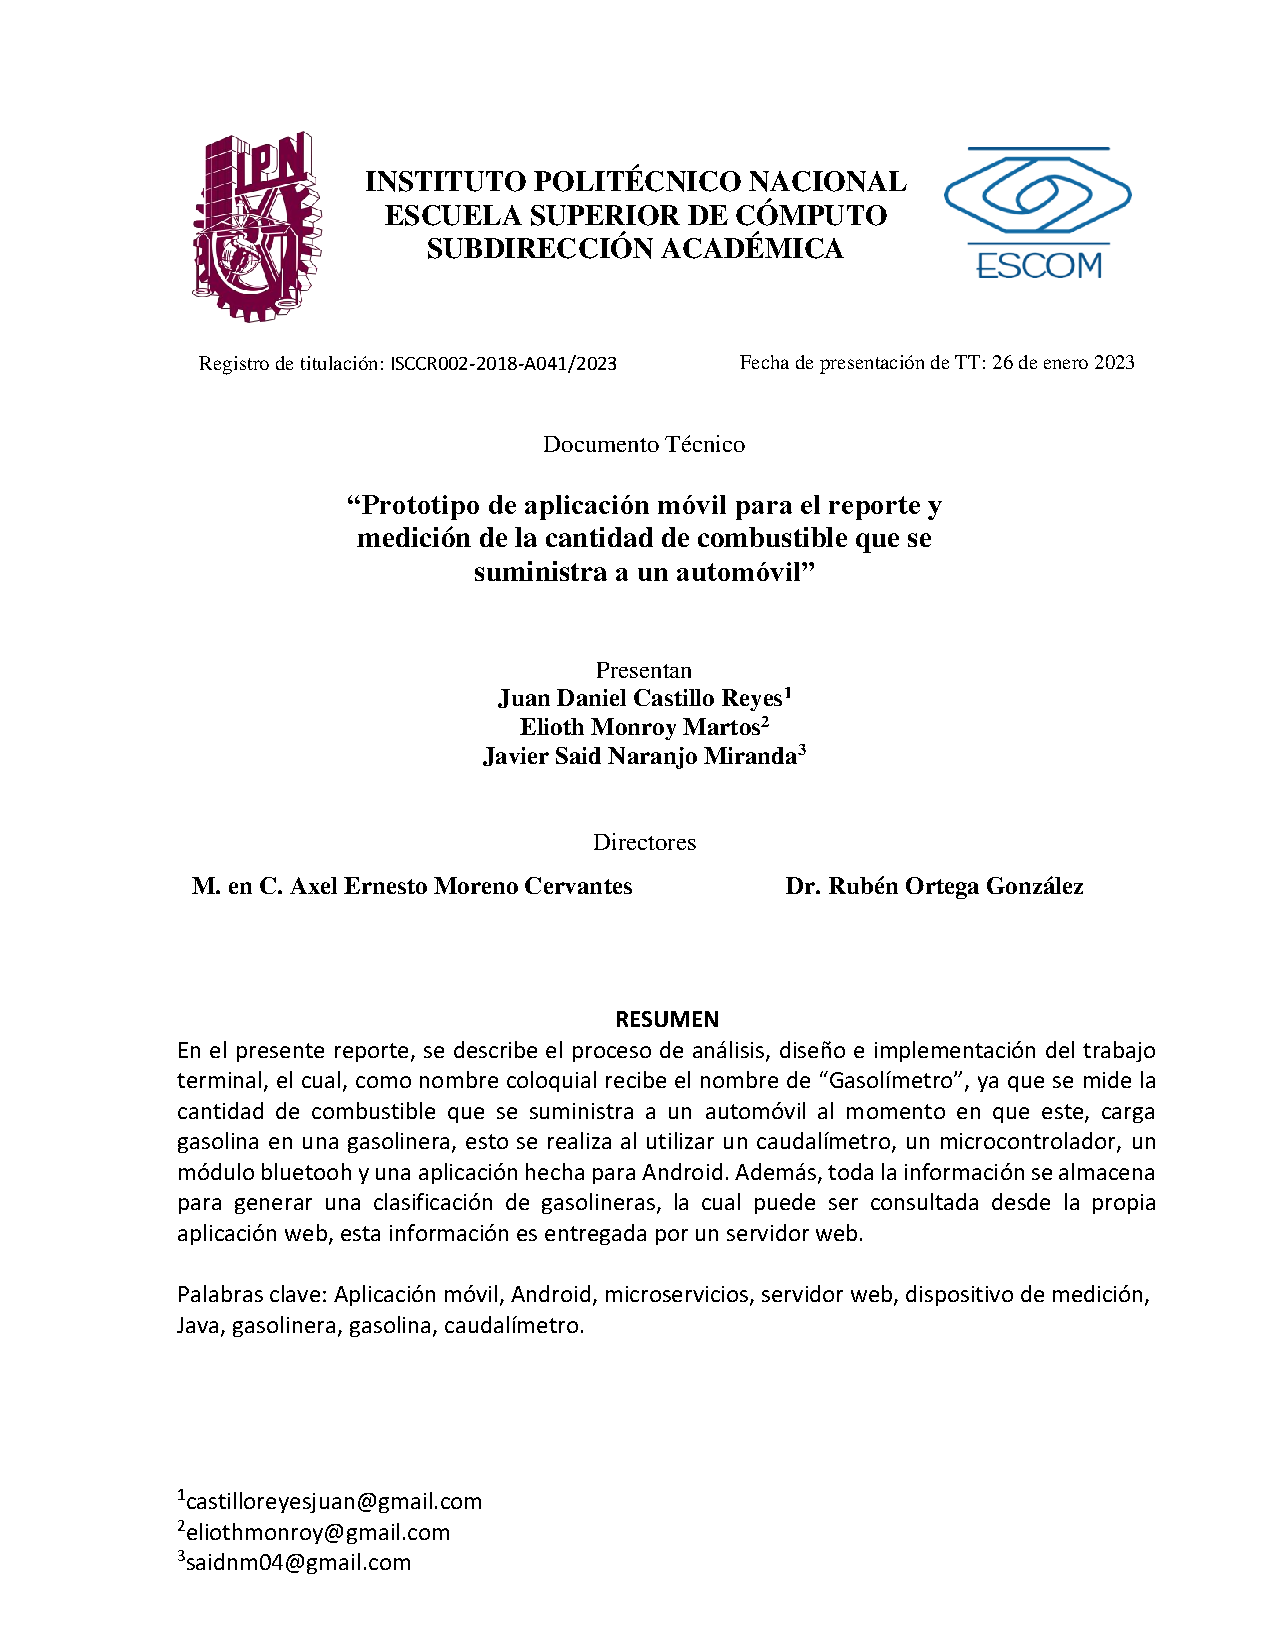
\includegraphics[scale=.78]{Disco/HojaPresentacion}
		\end{figure}
	}
	
\end{alwayssingle}

	
                   % Usada como hoja de presentación
 
\begin{comment}
\begin{dedication}
A la Facultad de Ingeniería y a la  Universidad, por la formación que me han dado.\\
Es gracias a ustedes que es posible el presente trabajo.\\
En verdad, gracias.\\
Yo.
\end{dedication}
\end{comment}

\begin{alwayssingle}
	{
		\pagestyle{empty}
		%\begin{center}
		\vspace{1.5cm}
		\begin{figure}[H]
			\centering
			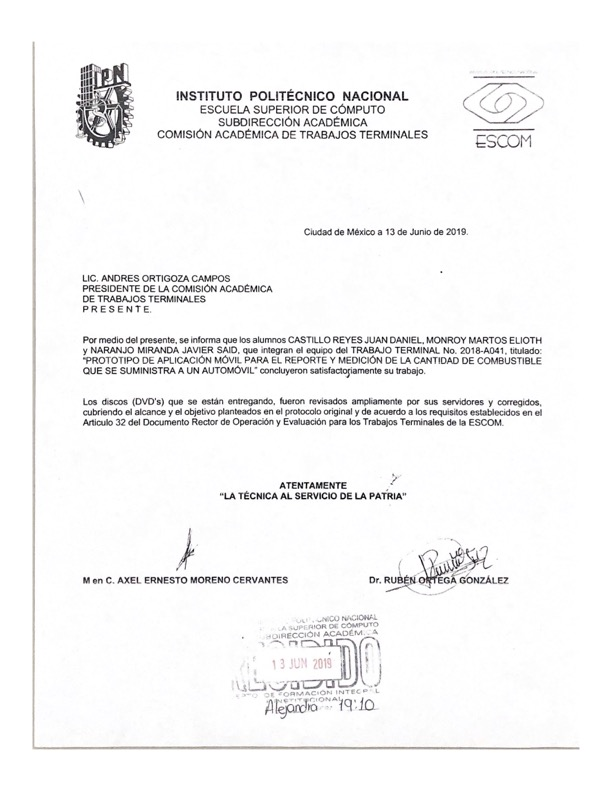
\includegraphics[scale=.4]{Disco/carta_responsiva}
		\end{figure}
		%\end{center}
		%\vspace{0.5cm}
	}
	
\end{alwayssingle}       % Usada como carta responsiva
 % ******************************* Thesis Declaration ********************************

\begin{comment}
\begin{declaration}

Por la presente declaro que, salvo cuando se haga referencia específica al trabajo de otras personas, el contenido de esta tesis es original y no se ha presentado total o parcialmente para su consideración para cualquier otro título o grado en esta o cualquier otra Universidad. Esta tesis es resultado de mi propio trabajo y no incluye nada que sea el resultado de algún trabajo realizado en colaboración, salvo que se indique específicamente en el texto. 
% Author and date will be inserted automatically from thesis.tex


\end{declaration}
\end{comment}

\begin{alwayssingle}
	{
	\pagestyle{empty}
	%\begin{center}
		\vspace{1.5cm}
		{
				%\noindent \textit{``Este documento contiene información desarrollada por la Escuela Superior de Cómputo del Instituto Politécnico Nacional, a partir de datos y documentos con derecho de propiedad y por lo tanto, su uso quedará restringido a las aplicaciones que explícitamente se convengan.''}\\
				%La aplicación no convenida exime a la escuela su responsabilidad técnica y da lugar a las consecuencias legales que para tal efecto se determinen.\\
				%Información adicional sobre este reporte técnico podrá obtenerse en:\\
				%La Subdirección Académica de la Escuela Superior de Cómputo del Instituto Politécnico Nacional, situada en Av. Juan de Dios Bátiz s/n Teléfono: 57296000, extensión 52000.
			\begin{figure}[H]
				\centering
				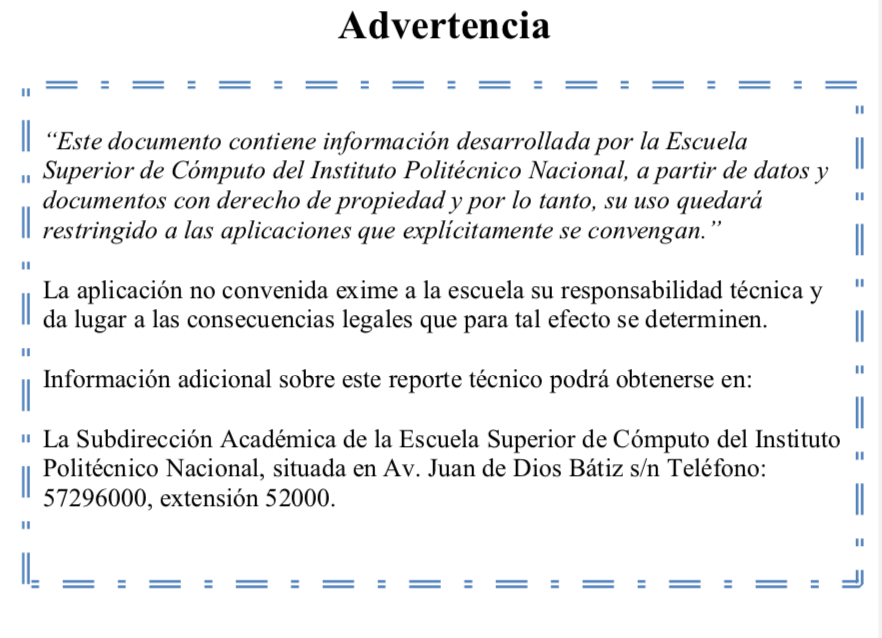
\includegraphics[scale=1.05]{Disco/advertencia}
			\end{figure}
		}
	%\end{center}
	%\vspace{0.5cm}
	}
\end{alwayssingle}
           % Advertencia
 %\chapter*{}
%\pagenumbering{Roman}

\begin{comment}
\begin{acknowledgements}

También quisiera reconocer a ... por ...CONACYT,  PAPIIT / etc.
\end{acknowledgements}
\end{comment}

\begin{alwayssingle}
	{
		\pagestyle{empty}
		%\begin{center}
		\vspace{1.5cm}
		{\chapter*{Agradecimientos}
			\noindent 
			\textit{``A mis padres por brindarme su apoyo incondicional incluso más allá de sus posibilidades.\\
			A mi hermano por que en el me veo reflejado en sus acciones.\\
			A mi familia por confiar siempre en mí y recordarme que todos estamos hechos para grandes cosas.\\
			A mi Alma por estar en todo momento conmigo.\\
			A mis compañeros de TT por el trabajo, la amistad y todas las experiencias vividas.\\
			A ESCOM por formar en mí un ingeniero en todos los sentidos de la palabra\\
			Al orejas por programar conmigo.''}
			\begin{flushright}
				Juan Daniel Castillo Reyes
			\end{flushright}
			\noindent 
			\textit{``A mi familia y amigos por el apoyo constante. Y a Tim Bergling (aka Avicii) por la inspiración.''}
			\begin{flushright}
				Elioth Monroy Martos
			\end{flushright}
			\noindent 
			\textit{``A mi familia, amigos y a mi novia.''}
			\begin{flushright}
				Javier Said Naranjo Miranda
			\end{flushright}
			
		}
		%\end{center}
		%\vspace{0.5cm}
	}
	
\end{alwayssingle}



   % Los agradecimientos



%%%%%%%%%%%%%%%%%%%%%%%%%%%%%%%%%%%%%%%%%%%%%%%%%%%%%
%                   ÍNDICES                         %
%%%%%%%%%%%%%%%%%%%%%%%%%%%%%%%%%%%%%%%%%%%%%%%%%%%%%
%Esta sección genera el índice
\setcounter{secnumdepth}{3} % organisational level that receives a numbers
\setcounter{tocdepth}{3}    % print table of contents for level 3
\tableofcontents            % Genera el índice 
%: ----------------------- list of figures/tables ------------------------
\listoffigures              % Genera el ínidce de figuras, comentar línea si no se usa
\listoftables               % Genera índice de tablas, comentar línea si no se usa


%%%%%%%%%%%%%%%%%%%%%%%%%%%%%%%%%%%%%%%%%%%%%%%%%%%%%
%                   CONTENIDO                       %
%%%%%%%%%%%%%%%%%%%%%%%%%%%%%%%%%%%%%%%%%%%%%%%%%%%%%
% the main text starts here with the introduction, 1st chapter,...
\mainmatter
\def\baselinestretch{1.5}                   % Interlineado de 1.5
%%%%%%%%%%%%%%%%%%%%%%%%%%%%%%%%%%%%%%%%%%%%%%%%%%%%%%%%%%%%%%%%%%%%%%%%%
%                    Descripción del documento                           %
%%%%%%%%%%%%%%%%%%%%%%%%%%%%%%%%%%%%%%%%%%%%%%%%%%%%%%%%%%%%%%%%%%%%%%%%%
\chapter*{Descripción del documento}
\addcontentsline{toc}{chapter}{Descripción del documento}  
%\section{Descripción del documento}
En el \textit{Capítulo \ref{chapter1} Introducción}, se expone de manera breve la motivación por la cual surgió el presente trabajo terminal, exponiendo el planteamiento del problema y los objetivos tanto generales como específicos que han sido planteados para el mismo.\\
En los capítulos siguientes se expresará a mayor profundidad el trabajo terminal, en el \textit{Capítulo \ref{chapter2} Marco conceptual} se presenta una referencia general, al ámbito bajo el cual es desarrollado el sistema, dando así, una introducción a los temas que son de interés para la correcta compresión de las diversas temáticas que abarca el trabajo terminal.\\
En el \textit{Capítulo \ref{chapter3} Análisis del sistema} se redactan los distintos factores tomados en cuenta para las selecciones de tecnología, se explican los motivos por los cuales fueron usados ciertos dispositivos de hardware y ciertas tecnologías, además de que se presenta una sustentación del sistema bajo los análisis de factibilidad y el análisis de riesgos.\\
El \textit{Capítulo \ref{chapter4} Diseño del sistema} se presenta el diseño de los distintos submódulos que componen al sistema, mostrando para la parte de hardware, los distintos diagramas de los circuitos que son usados, además, para la parte de software, se muestran los diagramas UML que permiten la construcción del sistema, entre los cuales se incluyen, diagramas de casos de uso, diagramas de secuencia y diagrama de clases. Finalmente, en este capítulo se muestra la arquitectura del sistema y el diagrama relacional de la base de datos.\\
Por último, el desarrollo del trabajo se explica en el \textit{Capítulo \ref{chapter5} Desarrollo del sistema} así como las pruebas para el mismo se exponen en el \textit{Capítulo \ref{chapter6} Pruebas del sistema}.\\
Las conclusiones obtenidas de este trabajo terminal se muestran en el \textit{Capítulo \ref{chapter7} Conclusiones} y el trabajo futuro en el \textit{Capítulo \ref{chapter8} Trabajo futuro}.\\

% this file is called up by thesis.tex
% content in this file will be fed into the main document
%----------------------- introduction file header -----------------------
%%%%%%%%%%%%%%%%%%%%%%%%%%%%%%%%%%%%%%%%%%%%%%%%%%%%%%%%%%%%%%%%%%%%%%%%%
%  Capítulo 1: Introducción- DEFINIR OBJETIVOS DE LA TESIS              %
%%%%%%%%%%%%%%%%%%%%%%%%%%%%%%%%%%%%%%%%%%%%%%%%%%%%%%%%%%%%%%%%%%%%%%%%%

\chapter{Introducción}\label{chapter1}

%: ----------------------- HELP: latex document organisation
% the commands below help you to subdivide and organise your thesis
%    \chapter{}       = level 1, top level
%    \section{}       = level 2
%    \subsection{}    = level 3
%    \subsubsection{} = level 4
%Cuando se use input, se debe poner la ruta desde el documento principal (o sea tesis.tex)
%%%%%%%%%%%%%%%%%%%%%%%%%%%%%%%%%%%%%%%%%%%%%%%%%%%%%%%%%%%%%%%%%%%%%%%%%
%                           Presentación                                %
%%%%%%%%%%%%%%%%%%%%%%%%%%%%%%%%%%%%%%%%%%%%%%%%%%%%%%%%%%%%%%%%%%%%%%%%%

\section{Presentación} % section headings are printed smaller than chapter names
El suministro de gasolina es una actividad que se realiza diariamente en miles de gasolineras de todo México, esta actividad consiste en la transmisión de gasolina al contenedor de combustible de un automóvil a través de una máquina dispensadora, dicho dispositivo registra la cantidad de gasolina suministrada (medida en litros) y muestra el equivalente en pesos a pagar según el precio del litro gasolina.
Dicha actividad es de suma importancia, ya que gran parte de las actividades económicas y personales en nuestro país dependen del uso de un vehículo cuyo funcionamiento requiera algún tipo de combustible. El proceso de suministro de gasolina depende de diversos factores, como lo son una serie de dispositivos electrónicos y mecánicos conectados entre sí, además de la interacción con la persona despachadora de la gasolina, todos estos factores influyen en la precisión con la que los litros de gasolina son suministrados a un vehículo.
\\
En los últimos años, la Profeco (Procuraduría Federal del Consumidor) ha detectado nuevas modalidades para el robo de gasolina, la mayoría de estas, sucede durante el proceso de recarga o suministro de gasolina, lo cuál, muchas veces suele pasar como un fenómeno desapercibido para el usuario final. 
Este problema, cobra especial relevancia en un país de consumo elevado de gasolina como México. Petróleos Mexicanos (PEMEX) informó que durante el primer semestre del año 2016 el consumo de gasolina fue de 812 mil barriles por día. Lo anterior equivale a 129 millones de litros diarios, de los cuales, 78 por ciento corresponde al tipo Magna y 22 por ciento al tipo Premium, según explica dicho órgano en su cuenta oficial de Twitter \cite{Pre1}.
Las cifras anteriores ubican a México entre los primeros consumidores de gasolina a nivel mundial. Además, en el año 2014 México ocupo la cuarta posición a nivel mundial en consumo de gasolina al día, solo por debajo de Estados Unidos, Japón y Canadá \citep{Pre2}.
\\
Otro factor importante en el consumo de gasolina es el precio, según el sitio Global Petrol Prices en el año 2018 México se encuentra entre los países latinoamericanos con los precios más elevados para el litro de gasolina ubicándose en 1.01 dólares por litro al término del primer semestre \citep{Pre3}.
\\
La estadística anterior cobra mayor relevancia cuándo se estudian los ingresos económicos del mexicano. Los mexicanos gastan en promedio un 3.38 por ciento de sus ingresos, unos 5 mil 336 pesos, en comprar 358.94 litros de gasolina al año, que es el promedio que utiliza un conductor en el país \citep{Pre4}.
\\
Basándonos en las estadísticas mencionadas con anterioridad observamos que el consumo de gasolina en México es una actividad de suma importancia y que afecta en buena parte las economías de las familias mexicanas. Dada la importancia económica de esta actividad las gasolineras cuentan con mecanismos de revisión que corroboran que el suministro de gasolina se realice de manera correcta en las gasolineras de país. Lamentablemente, muchas irregularidades se han presentado en los últimos años en diversas gasolineras, la mayoría de ellas tiene que ver con la exactitud al momento de despechar litros de combustible.
\\
Durante el 2014, la Procuraduría Federal del Consumidor –Profeco- revisó 1,792 gasolineras, de las cuales, el 56\% (1,017 estaciones) tuvieron alguna irregularidad. Esta cifra es sin contar a las 233 gasolineras que se negaron a ser verificadas y mejor pagaron la multa correspondiente.
En lo que va del año 2018, la Profeco ha revisado 400 estaciones de servicio, de las cuales 68\% (274 gasolineras) fueron inmovilizadas no sólo por no despachar completo sino por no contar con las señalizaciones adecuadas. Asimismo, 39 gasolineras se negaron a ser revisadas por lo que pagaron la multa de \$250,000 pesos \citep{Pre5}.
\\
Actualmente, la Profeco posee una lista negra con las gasolineras en las que se han encontrado irregularidades, sin embargo, dicha lista es actualizada después del periodo de revisiones lo cuál decrementa la exactitud de la lista debido a un periodo largo de actualización, además, cómo ya se mencionó existen gasolineras que evitan una revisión mediante el pago de una multa, lo cuál impide que exista una clasificación correcta de las gasolineras.
\\
La propuesta de solución planteada en este trabajo terminal consiste en la creación de una aplicación móvil que permita realizar una mejor clasificación de las gasolineras de acuerdo con su exactitud al momento de cargar gasolina. Dicha clasificación será actualizada constantemente con la ayuda de un sensor que medirá la cantidad de litros ingresados al vehículo, de esta forma, pondrán ser censadas todas aquellas gasolineras que evitan una revisión de la Profeco mediante el pago de una multa. Finalmente, la clasificación de las gasolineras no dependerá de una sola revisión, sino que será retroalimentada por las mediciones constantes de cada sensor presente en un automóvil al momento de cargar gasolina, lo cuál incrementa la exactitud en el algoritmo de clasificación.
%%%%%%%%%%%%%%%%%%%%%%%%%%%%%%%%%%%%%%%%%%%%%%%%%%%%%%%%%%%%%%%%%%%%%%%%%
%                           Motivación y estado del arte                %
%%%%%%%%%%%%%%%%%%%%%%%%%%%%%%%%%%%%%%%%%%%%%%%%%%%%%%%%%%%%%%%%%%%%%%%%%
\section{Motivación}
La posibilidad de pagar por litros de gasolina que estén incompletos ya es un riesgo que existe en todo el país. En los últimos años las autoridades han confirmado irregularidades en gasolinerías de las 32 entidades federativas. En promedio, cada tres días se descubre y sanciona una nueva gasolinera. \citep{Not1}
Entre 2005 y 2010 tres de cada 10 gasolineras presentaban alguna falla. En los últimos años esta relación se invirtió por completo: ahora, de cada 10 verificaciones, sólo en tres Profeco no halla irregularidades. \citep{Not2}
Teniendo en cuenta que no todas las gasolineras ofrecen litros de a litro a los consumidores se decidió realizar una aplicación móvil la cual permita a los usuarios conocer cuáles son las gasolineras que ofrecen realmente la cantidad de gasolina solicitada y a su vez cual es la cantidad de gasolina que está siendo cargada a su vehículo.
%%%%%%%%%%%%%%%%%%%%%%%%%%%%%%%%%%%%%%%%%%%%%%%%%%%%%%%%%%%%%%%%%%%%%%%%%
%                   Planteamiento del problema                          %
%%%%%%%%%%%%%%%%%%%%%%%%%%%%%%%%%%%%%%%%%%%%%%%%%%%%%%%%%%%%%%%%%%%%%%%%%

\section{Planteamiento del problema}
El desconocimiento por parte de los consumidores de gasolina de la cantidad real de combustible que es recargada en sus vehículos ha sido un factor importante para que las gasolineras no recarguen la cantidad solicitada en su totalidad. Este fenómeno ha aumentado con el tiempo y ahora son más los establecimientos que realizan recargan erróneas de combustible.
%%%%%%%%%%%%%%%%%%%%%%%%%%%%%%%%%%%%%%%%%%%%%%%%%%%%%%%%%%%%%%%%%%%%%%%%%
%                           Objetivo                                    %
%%%%%%%%%%%%%%%%%%%%%%%%%%%%%%%%%%%%%%%%%%%%%%%%%%%%%%%%%%%%%%%%%%%%%%%%%

\section{Objetivos}

\subsection{Objetivo general}
Este trabajo tiene por objetivo desarrollar un prototipo de aplicación móvil para el sistema operativo Android en su versión 5 o posteriores, la cual permita consultar una clasificación de las gasolineras de la CDMX, elaborada mediante la comparación de la cantidad de gasolina que fue cargada a un automóvil con la cantidad de gasolina que el conductor del mismo solicitó.
\subsection{Objetivos específicos}
\begin{enumerate}[label=\arabic*.]
    \item Desarrollar una aplicación móvil que permita la recepción a través del puerto Bluetooth del celular, de los datos provenientes de un sensor que mida el flujo de gasolina que entra a un tanque de un automóvil.
	\item Desarrollar una aplicación móvil que permita la comunicación con un servidor web a través de un API basada en la arquitectura REST.
	\item Desarrollar un servidor web que permita realizar la clasificación de las gasolineras registradas en el sistema con base en los datos recibidos a través de una aplicación móvil.
	\item Desarrollar una aplicación móvil que permita el registro de usuarios en el sistema, así como la asociación de estos con sus respectivos sensores.
	\item Desarrollar una aplicación móvil que indique las gasolineras más cercanas y con las mejores clasificaciones de acuerdo con la geolocalización de los usuarios.
	\item Implementar un dispositivo electrónico el cual permita medir el flujo de gasolina que entra al tanque de un automóvil al momento de recargar gasolina.
	\item Implementar un dispositivo electrónico que transmita información a una aplicación móvil a través de un módulo Bluetooth.
\end{enumerate}
%%%%%%%%%%%%%%%%%%%%%%%%%%%%%%%%%%%%%%%%%%%%%%%%%%%%%%%%%%%%%%%%%%%%%%%%%
%                           Estado del arte                              %
%%%%%%%%%%%%%%%%%%%%%%%%%%%%%%%%%%%%%%%%%%%%%%%%%%%%%%%%%%%%%%%%%%%%%%%%%
\section{Estado del arte}
El problema de la exactitud al momento de suministrar combustible en una gasolinera ya ha sido abordado anteriormente por diversas instituciones tanto públicas como privadas.\\

Actualmente, existen 3 proyectos que tienen una funcionalidad similar a la propuesta en el presente Trabajo Terminal:
\begin{itemize}
	\item Full Me
	\item Zenzzer
\end{itemize}

La Tabla \ref{tabla_estado_arte} muestra un resumen de las características y precio de los sistemas mencionados.
\begin{longtable}{|M{1.7cm}|M{4cm}|M{4.2cm}|M{1.6cm}|M{2.3cm}|}
	\hline
	\textbf{Producto o sistema} & \textbf{Descripción} & \textbf{Características} & \textbf{Precio}& \textbf{Estado actual}  \\ \hline
	Full Me & Dispositivo electrónico que mide el flujo de combustible entrante en un tanque de gasolina de un automóvil, los resultados de la medición se pueden consultar mediante una aplicación móvil y la misma permite compartir los resultados en redes sociales. & 
	%Caracteristicas
	\begin{itemize}
		\item Dispositivo electromecánico de medición de flujo
		\item Interfaz de comunicación bluetooth
		\item Aplicación Android
		\item Compartes el resultado de la medición en redes sociales
		\item Sensor: Dispositivo cilíndrico de 12 cm de largo
	\end{itemize}
	& Sin información
	& Desarrollado como un prototipo de emprendimiento, no se encuentra en venta actualmente. \\ \hline
	Zenzzer & Aplicación móvil que funciona como una red social para automovilistas, donde los mismos pueden consultar y compartir información sobre las gasolineras que visitan. La información es desplegada a los usuarios en un mapa interactivo. Además de la aplicación, es posible comprar un dispositivo llamado ZenzMetter el cual se conecta a la computadora del automóvil para obtener información sobre el mismo, la cual es mostrada en una aplicación móvil.
	&
	\begin{itemize}
		\item Aplicación móvil disponible para Android 5.0 y posteriores
		\item Conexión al puerto OBD2 del automóvil
		\item Clasificación de las gasolineras por medio del precio de la gasolina
		\item Permite visualizar en la aplicación la cantidad de litros cargados en tiempo real
		\item Permite dejar comentarios de las gasolineras visitadas
		\item Compatible con solo 20 modelos de vehículos
	\end{itemize}
	& Aplicación móvil: Gratuita. ZenzMetter: 1000 pesos.
	& La empresa sigue en el mercado actualmente aunque solo es posible descargar la aplicación. El sensor ya no esta a la venta.
	\\ \hline
	Propuesta de sistema para medición de volumen de gasolina vía bluetooth &
	El trabajo consta de un sensor de flujo que recauda la información en bruto del flujo de gasolina que pasa, una placa “Arduino Uno” que procesa los datos para enviarlos a el modulo Bluetooth y una aplicación Android, la cual muestra la información de la medición.
	&
	\begin{itemize}
	\item Sensor de flujo modelo YF-S201
	\item Aplicación móvil disponible para Android.
	\item Módulo Bluetooth ZS-040
	\item Microcontrolador Arduino Uno
	\item Muestra los datos del volumen leído por el sensor en la aplicación Android
	\end{itemize}
	&
	320 pesos
	&
	Solo fue desarrollado como un proyecto de académico en el año 2016.
	\\ \hline
	Trabajo Terminal 2018-A041 (Solución Propuesta) & Aplicación móvil que muestre la clasificación de gasolineras elaborada mediante la información obtenida de un sensor conectado al tanque de gasolina de un automóvil, esta clasificación se muestra en un mapa el cual se ajusta a la ubicación del usuario para así solo mostrar las gasolineras que se encuentren cercanas a él. 
	&%Caracteristicas
	\begin{itemize}
		\item Aplicación móvil disponible para Android 5.0 y versiones posteriores
		\item Mapa interactivo que muestra las gasolineras mejor calificadas según la precisión de carga de combustible.
		\item Sensor de flujo de gasolina modelo FS400A-G.
		\item Visualización de la cantidad de combustible cargado en la aplicación.
		\item Uso de geolocalización para mostrar las gasolineras mejor calificadas cerca de la ubicación del usuario.
	\end{itemize}
	& Sensor: 700 pesos. Aplicación móvil: Gratuita.&
	Actualmente se encuentra en desarrollo. \\ \hline
	\caption{Estado del arte}
	\label{tabla_estado_arte}
\end{longtable}

%%%%%%%%%%%%%%%%%%%%%%%%%%%%%%%%%%%%%%%%%%%%%%%%%%%%%%%%%%%%%%%%%%%%%%%%%
%                           Marco Conceptual                               %
%%%%%%%%%%%%%%%%%%%%%%%%%%%%%%%%%%%%%%%%%%%%%%%%%%%%%%%%%%%%%%%%%%%%%%%%%

\chapter{Marco conceptual}\label{chapter2}
El presente Trabajo Terminal tiene como objetivo el desarrollo de un prototipo de aplicación para el sistema operativo Android que permita la clasificación de las gasolineras de la Ciudad de México a partir de la implementación de un algoritmo computacional, el cuál, utilizará las mediciones de diferentes sensores de flujo los cuáles enviarán sus datos a través de un módulo Bluetooth.
\paragraph{}
Dado que este trabajo terminal emplea conceptos de diversas áreas de la Ingeniería en Sistemas Computacionales, resulta fundamental dar una serie de definiciones previas que permitan un mejor entendimiento del documento.

\section{Gasolineras y su funcionamiento}
Primeramente, es necesario conocer los conceptos relacionados con una gasolinera, así como el estado actual de estos establecimientos en nuestro país.
\paragraph{}
Comenzaremos con la definición de gasolinera o estación de servicio. En el español general, la voz más usual para referirse al ‘depósito de gasolina para la venta al público’ o al ‘establecimiento donde se vende gasolina’ es gasolinera \citep{MarcoTeorico1}. 

Una vez que se ha identificado el concepto de gasolinera podemos empezar a citar datos estadísticos que concuerden con estos establecimientos, a continuación, se citan algunas cifras importantes que nos dan un panorama del número de gasolineras en el país y su relación con respecto al número de automóviles en circulación. En el año 2017 se registraron más de 12,000 gasolineras en todo México, estos establecimientos dan servicio a aproximadamente 43 millones de vehículos en circulación, es decir,  que cada gasolinera debe abastecer a cerca de 3,652 vehículos.  Traducido de otra forma, hay en promedio una gasolinera por cada 10 mil 514 habitantes, de acuerdo a la Comisión Reguladora de Energía (CRE)\citep{MarcoTeorico2}.
\paragraph{}
Siendo un poco más específicos, en la Ciudad de México hay 4.6 millones de autos y menos de 500 estaciones de servicio, así, cada gasolinera debe atender en promedio a 11 mil 400 vehículos. Una de las principales razones por las cuáles el número de gasolineras resulta relativamente bajo tiene que ver con las normas que rigen la construcción y mantenimiento de las Estaciones de Servicio en México \citep{MarcoTeorico2}, pues los requerimientos necesarios para la creación de una nueva gasolinera son numerosos. Es así, que resulta importante estudiar los normas para la construcción y operación de las gasolineras en México.

\paragraph{NOM-005-ASEA-2016}
En México, la norma que rige el diseño, construcción, operación y mantenimiento de Estaciones de Servicio para almacenamiento y expendio de diésel y gasolinas en la NORMA Oficial Mexicana NOM-005-ASEA-2016, la cual, es emitida por la Agencia Nacional de Seguridad Industrial y de Protección al Medio Ambiente del Sector Hidrocarburos. Dicha norma tiene como objetivo establecer las especificaciones, parámetros y requisitos técnicos de Seguridad Industrial, Seguridad Operativa, y Protección Ambiental que se deben cumplir en el diseño, construcción, operación y mantenimiento de Estaciones de Servicio para almacenamiento y expendio de diésel y gasolinas.

Tomando como referencia la NOM-005 daremos una introducción a los elementos que se usan dentro de una gasolinera para el proceso de suministro y recarga de combustible.
El proceso de suministro de gasolina comienza cuando un vehículo accede a una estación de servicio y realiza una maniobra de frenado junto a un módulo de despacho. Según la NOM-005 un módulo de despacho es un elemento junto al cual el vehículo o embarcación se abastecen de combustible a través de un dispensario. El dispensario o expendedor de gasolina es el sistema automático usado para la medición y despacho de gasolina y otros combustibles líquidos \citep{NORMA-005}.
Posteriormente, personal competente realiza transmisión de combustible del expendedor de gasolina al tanque del automóvil para que finalmente, el usuario realice el pago correspondiente por la cantidad de combustible que fue ingresado al vehículo.

\paragraph{El dispensador de combustible}
Ahora que se ha definido el proceso de suministro de gasolina, es necesario definir algunos de los elementos que intervienen en él, se hará énfasis en aquellos conceptos relacionados con la medición de combustible, ya que esta variable influye de manera directa en el presente trabajo.

Históricamente, el primer dispensador de combustible fue creado por Sylvanus Bowser el 5 de septiembre de 1885 en Indiana Estados Unidos \citep{MarcoTeorico4}. Dicho dispensador no era usado para para automóviles debido a la poca comercialización que existía, en su lugar era utilizado para recargar lámparas de keroseno y estufas. El primer dispensador de combustible fue patentado por el noruego John J. Tokheim en 1901. El gigante de la industria minorista de combustibles Tokheim-OPW, recibió su nombre es honor a este científico. \citep{MarcoTeorico4}

El elemento principal para el suministro de gasolina es el dispensador de combustible, el cuál, se compone de dos partes principales: la unidad de control electrónica, que contiene un sistema embebido para controlar la acción de la bomba y que se comunica con el sistema del mostrador, y en segundo lugar, una sección mecánica que contiene una bomba eléctrica y unas válvulas para bombear físicamente el combustible. 
\\Los dispensadores más modernos están equipados normalmente con un sistema de control de recuperación de vapores, para evitar que los vapores de la gasolina se escapen hacia el aire de la gasolinera.

A lo largo de la historia, los dispensadores de combustible han tenido una gama muy amplia de diseños para resolver los problemas mecánicos del bombeo, la medición confiable, la seguridad y la estética.\\\\

En la Figura \ref{fig:diagrama_dispensador} se observa un diagrama general de un dispensador de combustible.
\begin{figure}[H]
	\centering
	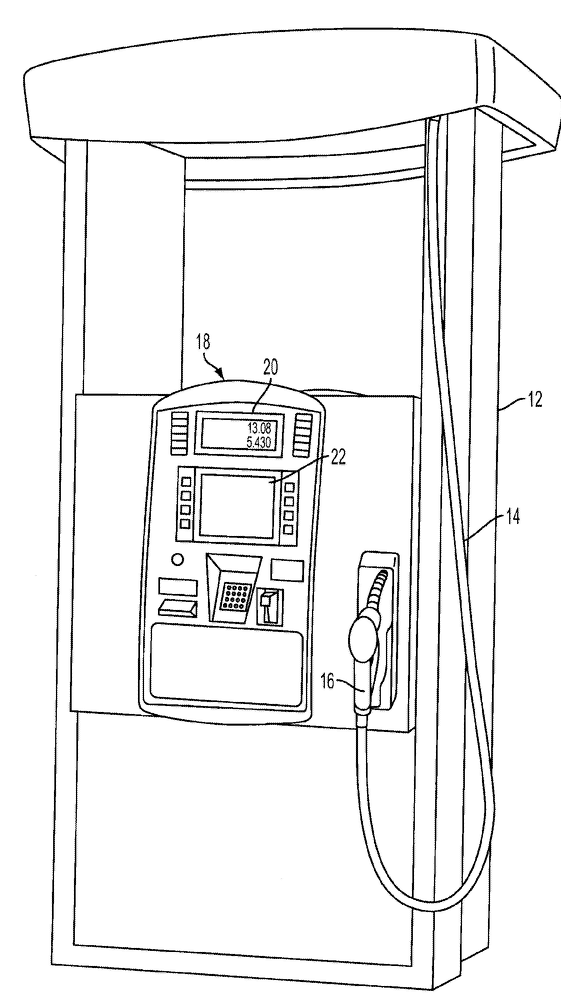
\includegraphics[scale=.25]{Capitulo2/images/diagrama_dispensador}
	\caption{Patente de dispensador de combustible}
	\label{fig:diagrama_dispensador}
\end{figure}

\paragraph{Mediciones de un dispensador de gasolina}
Una de las funciones más importantes de una del dispensador de combustible en una estación de servicio, es la medición precisa y consistente del flujo y volumen despachado. Esta medición es realizada comúnmente por un medidor volumétrico de operación mecánica, conectado a un panel electrónico que contabiliza el volumen y realiza la conversión hacia la moneda local para finalmente cobrar al consumidor \citep{MarcoTeorico3}.

\paragraph{Medidor de compresión de pistones}La medición de flujo casi siempre se realiza mediante un medidor de 4 pistones conectado a un codificador electrónico. Las bombas de combustible convierten el movimiento del medidor en impulsos eléctricos utilizando un codificador rotatorio \citep{MarcoTeorico5}.

\begin{figure}[H]
	\centering
	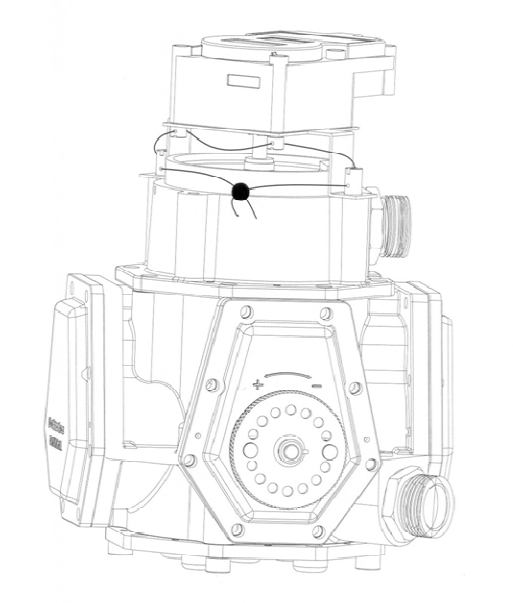
\includegraphics[scale=.4]{Capitulo2/images/medidor_gasolina}
	\caption{Medidor de 4 pistones de la empresa Petrotec}
	\label{fig:medidor_gasolina}
\end{figure}

\paragraph{Codificador rotatorio}
Un codificador rotatorio es un dispositivo electromecánico que convierte la posición angular de un eje, directamente a un código digital, estos dispositivos son considerados como transductores \citep{MarcoTeorico6}.

\begin{figure}[H]
	\centering
	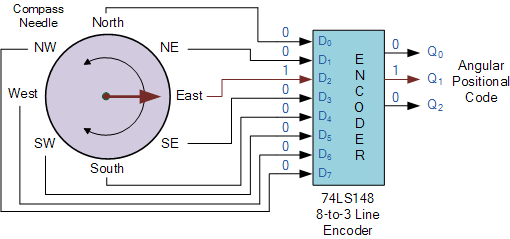
\includegraphics[scale=.8]{Capitulo2/images/electronic_encoder}
	\caption{Diagrama interno de un codificador rotatorio}
	\label{fig:electronic_encoder}
\end{figure}

\paragraph{Sistema embebido del dispensador}
Una vez que el codificador rotatorio ha empezado a registrar un movimiento angular los impulsos que éste emite son enviados al sistema embebido del dispensador de combustible, dicho sistema se encarga de realizar el cómputo de las señales recibidas, el estudió de esta unidad computacional resulta extenso ya que es el encargado de realizar toda la parte electrónica del dispensador de gasolina, por lo que a continuación se muestra una imágen de una placa que la empresa Gasboy utiliza para los dispensadores de gasolina que comercializan.

\begin{figure}[H]
	\centering
	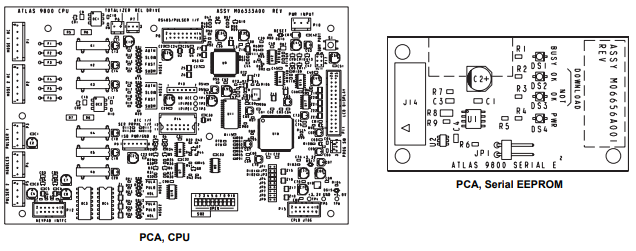
\includegraphics[scale=.8]{Capitulo2/images/pca_gasboy}
	\caption{Printed Circuit Assembly de la empresa Gasboy para dispensadores de gasolina}
	\label{fig:pca_gasboy}
\end{figure}

\paragraph{Pistola de combustible}
Las pistolas están conectadas a la bomba a través de mangueras flexibles, lo que permite colocarlas en la entrada de llenado del vehículo. Las mangueras son robustas para resistir el desgaste intenso, incluida la exposición a la intemperie y el arrastre, y a menudo se unen utilizando resortes pesados o arreglos de bobina para proporcionar resistencia adicional.

\begin{figure}[H]
	\centering
	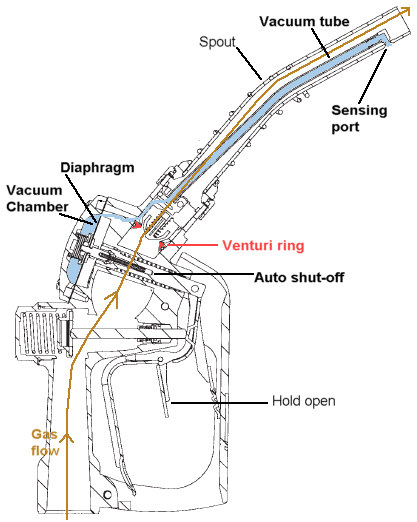
\includegraphics[scale=.6]{Capitulo2/images/nozzle}
	\caption{Pistola de combustible y sus componentes}
	\label{fig:nozzle}
\end{figure}

A continuación se enlistan los pasos que describen el funcionamiento de una pistola de combustible, además se muestra una tabla con las características técnicas de una pistola de la marca estadounidense Husky.

\begin{itemize}
	\item El dispensador es activado presionando el pivote con la marca Hold open.
	\item La pistola de combustible se encuentra presurizada y la gasolina empieza a fluir a través del cuerpo de la pistola.
	\item La gasolina entra en contacto con el anillo Venturi y provoca que la válvula contra derrames sea activada.
	\item Mientras la gasolina fluye a través del cuerpo de la pistola el tubo de vacío (Vacuum tube en la figura) aspira aire debido a un efecto de baja presión.
	\item Cuando el nivel de gasolina cubre el área de la figura marcada como Sensing port este no puede seguir ingresando aire lo que provoca que el diafragma sea activado cerrando el paso de gasolina.
\end{itemize}

\paragraph{Funcionamiento de una pistola de combustible}
Los pasos listados anteriormente fueron obtenidos de un vídeo hecho por el presidente de la Compañia Husky, Grenville Sutcliffe, dicho recurso puede ser consultado en el link de la cita correspondiente \citep{MarcoTeorico8}.
\paragraph{}
Especificación de una pistola de combustible de la Marca Husky
\begin{longtable}{|M{7cm}|M{7.5cm}|}
	\hline
	\textbf{Característica} & \textbf{Valor}
	\\\hline
	Tipo & Husky X-Mate
	\\\hline
	Material & Cuerpo de alumino, Recubrimiento de teflón, Sellos de Viton,
	Vástago de acero inoxidable
	\\\hline
	Rango de flujo & 8~60 litros/min
	\\\hline
	Diametro del canal & 20.6mm (13/16th")
	\\\hline
	Presión(min) & 2.4 PSI (160mBar)
	\\\hline
	Presión(max) & 50 PSI (3.35Bar)
	\\\hline
	Rango de temperatura & -6 C to +55 C
	\\\hline
	Conexiones & 3/4 BSP(F)
	\\\hline
	\caption{Características de una pistola de combustible}
	\label{tabla_pistola_combustible} 
\end{longtable}

\paragraph{Consideraciones para la medición}
En los EE. UU., la cantidad de flujo está limitada a 10 galones por minuto (37.9 litros) para automóviles y 40 galones por minuto para camiones. Este caudal se basa en el diámetro del tubo de llenado de combustible del vehículo, que limita el flujo a estas cantidades. Aunque la medidas de velocidad de flujo anteriores fueron determinadas por el National Institute of Standards and Technology de los Estados Unidos, éstas serán utilizadas en el presente trabajo, ya que los modelos de los automóviles que fueron usados para las pruebas tienen una presencia mayoritaria en nuestros país \citep{MarcoTeorico7}.
\paragraph{}
Derivado de lo anterior se deberá buscar un sensor que soporte las mismas especificaciones de presión, cantidad de flujo y pulsos de salida que los componentes que conforman a dispensador de gasolina, esto con la finalidad de obtener mediciones lo más cercanas posibles a la realidad al momento de implementar nuestro proyecto.
\section{Sensores}
En la sección anterior observamos que para hacer la mediciones de los litros de gasolina que son ingresados a un automóvil se hace uso de diferentes sensores. De igual forma, en el objetivo del presente trabajo se plantea el uso de un sensor de flujo para las mediciones en el proceso de suministro de gasolina, es por eso, que a continuación se define el concepto de sensor.
\\
Los sensores, son los elementos que se encuentran en contacto con una planta, y tienen una salida que depende de alguna manera de la variable que está siendo medida o monitoreada \citep{MarcoTeorico10}. Si existe más de un elemento de sensado o monitoreo dentro del sistema, él elemento que se encuentre en contacto directo con la planta generadora de las variables recibe el nombre de “elemento principal de medición”, lo otros son elementos secundarios de medición.
\\
Un sensor es todo aquello que tiene una propiedad sensible a una magnitud del medio, y al variar esta magnitud también varia con cierta intensidad la propiedad, es decir, manifiesta la presencia de dicha magnitud, y también su medida.

\subsection{Sensor de flujo}
La medición de la tasa de flujo de un material a través de tuberías es extremadamente importante en
una amplia gama de industrias, incluyendo la industria química, del petróleo, del acero, de alimentos servicios públicos, entre otros. \citep{MarcoTeorico10}
Hay un gran número de medidores de flujo en el mercado. 
\\
El sensor de flujo es un dispositivo que, instalado en línea con una tubería, permite determinar cuándo está circulando un líquido o un gas. Estos son del tipo apagado/encendido ya que  determinan cuándo está o no circulando un fluido, pero no miden el caudal. Para medir el caudal se requiere un caudalímetro.

\begin{figure}[H]
	\centering
	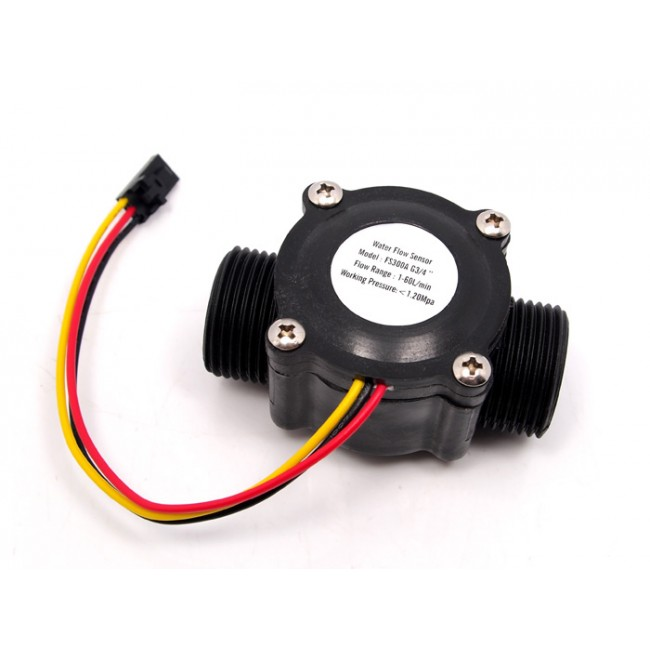
\includegraphics[scale=.4]{Capitulo2/images/flowmeter}
	\caption{Sensor de flujo de Efecto Hall}
	\label{fig:flowmeter}
\end{figure}

\paragraph{Caudalímetro}
Un caudalímetro es un instrumento de medida para la medición de caudal o gasto volumétrico de un fluido. También suelen llamarse medidores de caudal, medidores de flujo o flujómetros \citep{MarcoTeorico10}.

A continuación, se muestra una lista con los tipos de caudalímetros más comunes en el mercado:
\begin{itemize}
	\item Caudalímetro de diferencial de presión. Estos son los caudalímetros industriales más comunes para líquidos y gases limpios. \citep{MarcoTeorico10}
	\item Caudalímetro Mecánico. Consisten en un molino cuyas aspas están transversales a la circulación de fluido. El flujo hace girar el molino cuyo eje mueve un contador que acumula lecturas.
	\item Caudalímetro Vortex
	\item Caudalímetro Mecánico
\end{itemize} 
\section{Comunicación inalámbrica}
\subsection{Protocolo Bluetooth}
Bluetooth es una tecnología de conectividad inalámbrica de baja potencia que se utiliza para
transmitir audio, transferir datos y transmitir información entre dispositivos. Hay dos sabores
de la tecnología Bluetooth, velocidad básica / velocidad de datos mejorada (BR / EDR) y baja
energía (LE) \citep{Bluetooth}.
\subsection{WiFi}
WiFi es la abreviatura o el nombre comercial de Wireless Fidelity y, como su nombre lo indica,
es un sistema de conexión de ordenadores completamente inalámbrico, que permite a sus usuarios
compartir y transferir información utilizando ondas de radio, es decir, sin utilizar cableado alguno.
De esta manera, podemos mantener comunicaciones entre ordenadores, portátiles, móviles y otros
dispositivos que cuenten con tecnología de recepción inalámbrica, facilitando enormemente las
comunicaciones, incluso en lugares abiertos lejos de nuestras casas y ocinas. Las redes WiFi por
lo general son de libre acceso, a menos que estén protegidas mediante contraseñas, lo cual, indicará
que son unas redes privadas utilizadas para conexiones con redes locales (LAN)\citep{WiFi}.
%\subsection{Módulo Bluetooth}
%\subsection{Protocolo HTTP}
%\section{Aplicación Móvil}
%\subsection{Sistema Operativo Android}
\section{Arquitectura de microservicios}
A continuación, se presentan los conceptos más importantes de la arquitectura de software que será utilizada para el presente proyecto, la cuál, recibe el nombre de Arquitectura de Microservicios.
\paragraph{Patrón de arquitectura}
Los patrones arquitectónicos, o patrones de arquitectura, también llamados arquetipos ofrecen soluciones a problemas de arquitectura de software en ingeniería, además, ayudan a definir las características básicas y de comportamiento de una aplicación. Por ejemplo, algunos patrones de arquitectura naturalmente se prestan hacia aplicaciones altamente escalables, mientras que otros patrones de arquitectura se prestan naturalmente hacia aplicaciones que sean altamente ágiles \citep{MarcoTeorico9}.
\\
Actualmente, existen diversos patrones de arquitectura de software, enseguida, se listan algunos de los más populares:
\begin{itemize}
	\item Arquitectura N-capas
	\item Arquitectura Orientada a Eventos
	\item Arquitectura Micro-kernel
	\item Arquitectura de Microservicios
\end{itemize}

\paragraph{}
En la actualidad, la Arquitectura de Microservicios está ganando terreno rápidamente en la industria como una alternativa viable a las arquitecturas monolíticas y orientadas a servicios \citep{MarcoTeorico9}.

\paragraph{Component decoupling}
El primer concepto importante dentro de la arquitectura de microservicios es el de 'Separately deployment units'. Este concepto nos dice que dentro de una aplicación de software, se debe buscar es desacoplamiento de los componentes, de manera que cada unidad mínima de funcionalidad pueda ser puesta en producción de manera independiente, y sin que esta afecte a otras unidades.

\paragraph{Service component} Quizás el concepto más importante para entender con este patrón, es la noción de un componente de servicio. Estos componentes pueden variar en tamaño o granularidad (independencia con otros componentes), yendo desde un módulo sencillo hasta ocupar una gran parte de la aplicación. 
\\
Los componentes de servicio contienen uno o más módulos (por ejemplo, clases de Java) que representan una funcionalidad del sistema (por ejemplo, proporcionar el clima para un determinado
ciudad o pueblo). Diseñar el nivel correcto de granularidad de un componente de servicio es uno de los mayores retos dentro de una arquitectura de microservicios \citep{MarcoTeorico9}.

\paragraph{Distributed architecture}
Todos los componentes de esta arquitectura se encuentran totalmente desacoplados, además, son accedidos a través de un mecanismo de control de acceso remoto como REST, SOAP o RMI.

La naturaleza distribuida de este patrón de arquitectura es la forma en que logra su escalabilidad y características de despliegue superiores a las de otras arquitecturas \citep{MarcoTeorico9}.

\begin{figure}[H]
	\centering
	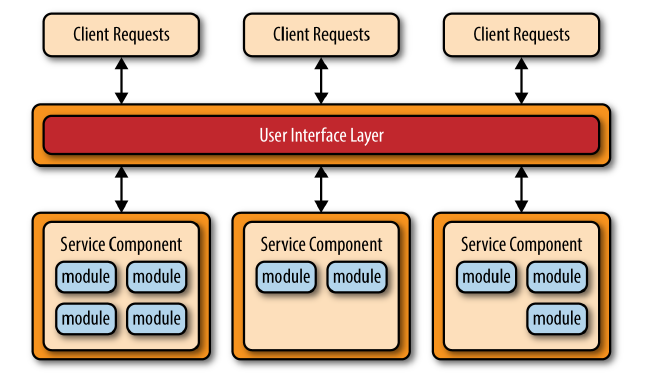
\includegraphics[scale=.6]{Capitulo2/images/microservicios}
	\caption{Arquitectura básica de microservicios}
	\label{fig:microservicios}
\end{figure}

\paragraph{Avoid dependencies and orchestration}
Uno de los principales retos de la arquitectura de microservicios es determinar el valor correcto de granularidad para los componentes de servicio. Si los componentes tienen un alto acoplamiento entre ellos, los beneficios de esta arquitectura no podrán ser aprovechados, por otro lado, si los componentes tiene una granularidad muy alta será necesario agregar un servicio de administración para dichos componentes llamado Orchestration. El problema de una granularidad alta, radica en que los diferentes servicios necesitarán una forma de comunicarse entre ellos, este fenómeno recibe el nombre de Interservice Communication, y provoca un alto acoplamiento entre componentes \citep{MarcoTeorico9}.
\\
Una forma de solventar el alto acoplamiento es mediante una base datos compartida entre los diferentes servicios de la aplicación.

\subsection{API REST}
Una API REST es una interfaz de comunicación basada en un conjunto de restricciones que permiten la comunicación maquina a maquina, el presente trabajo plantea el uso de un API REST por lo que es importante definirla y dar un contexto general de su uso.

\paragraph{Web service} Para poder definir un API REST es necesario dar un conjunto de conceptos previos. Un término que sale a relucir al hablar del tema es el de Servicio Web.
\\
Un servicio web es un término genérico para una función de software interoperable de máquina a máquina que se aloja en una dirección accesible de la red \citep{MarcoTeorico11}.
\\
Un servicio web, tiene una interfaz que oculta los detalles de su implementación, de esta forma, podrán usarse de forma independientemente de la plataforma de hardware o software en la que se haya implementado, e independientemente del lenguaje de programación en el que está escrito. Esta independencia fomenta que las aplicaciones basadas en servicios web tengan un bajo acoplamiento, sean orientadas a componentes, y permitan la comunicación entre diferentes tecnologías \citep{MarcoTeorico11}.

\begin{figure}[H]
	\centering
	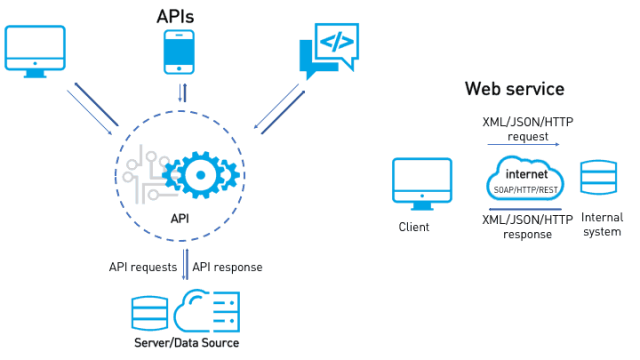
\includegraphics[scale=.6]{Capitulo2/images/web_service}
	\caption{Ejemplo de uso de los web services}
	\label{fig:web_service}
\end{figure}

En la actualidad, existen dos protocolos que son ampliamente usados para la implementación de servicios web:
\begin{itemize}
	\item SOAP (Simple Access Object Protocol)
	\item Protocolos JSON 
\end{itemize}

\paragraph{SOAP}
Un servicio web basado en SOAP posee una interfaz de comunicación descrita en un formato conocido como Web Service Definition Language (WSDL). A su vez, un servicio web SOAP es escrito usando una notación formal de XML, esta notación posee diversa información como Formatos de Mensaje, Protocolos de transporte y Ubicación. Existen herramientas que pueden ser usadas para procesar un WSDL y producir programas cliente capaces de comunicarse con el servicio utilizando el protocolo SOAP basado en XML. Aunque SOAP puede ser un protocolo de comunicación detallado, tiene la ventaja de la extensibilidad y esto hace que sea altamente usado en entornos empresariales \citep{MarcoTeorico11}.

\paragraph{JSON}
Un servicio web basado en el formato JSON utiliza el protocolo HTTP para establecer una comunicación, este protocolo es considerado menos formal que el uso del protocolo SOAP. Este tipo de servicios web es utilizado comúnmente para la comunicación con aplicaciones móviles gracias a la sencillez del protocolo \citep{MarcoTeorico11}.
 
\paragraph{Contraste}En contraste, un servicio web basado en SOAP agregar una capa de extensibilidad que es ideal para aplicaciones empresariales, pero pagando el precio de ser un protocolo bastante robusto y formal a la hora de escribir sus definiciones lo que implica un costo elevado de análisis y desarrollo, por otro lado, un servicio web basado en JSON permite un desarrollo ágil al utilizar un protocolo relativamente ligero como HTTP, sin embargo, su misma sencillez evita una formalidad al momento de adaptarlo al negocio, por lo que es recomendable utilizarse como puente de comunicación entre dispositivos.

Diferencias entre servicios web SOAP vs JSON \citep{MarcoTeorico11}:

\begin{itemize}
	\item El contenido de un mensaje SOAP esta en formato XML, mientras que un mensaje JSON contiene datos en formato JSON. JSON y XML son diferentes mecanismos de codificación para describir datos estructurados.
	\item JSON es un mecanismo de codificación bastante eficiente, por lo que los mensajes escritos tienden a ser mucho más pequeños que sus mensajes equivalentes en XML.
	\item JSON es un formato muy usado para aplicaciones móviles debido a su integración con Javascript, es por eso que es el mecanismo ideal para apps móviles.
	\item SOAP proporciona un mecanismo para agregar encabezados a un mensaje y una familia de especificaciones para la calidad del servicio (como la configuración de seguridad y las transacciones distribuidas). JSON no proporciona este mecanismo. En su lugar, se basa en los servicios del protocolo de red HTTP subyacente.
	\item Los servicios web basados en SOAP son descritos mediante un documento WSDL.
	\item Los servicios web SOAP tienen un formato de error explícito que implica el uso de mensajes de error SOAP. No hay equivalente para JSON.
	\item Los servicios web de JSON son compatibles tanto con una interfaz RESTful como con una interfaz Request-Response, SOAP solo es compatible con la interfaz de Request-Response. 
\end{itemize}

\paragraph{REST}
Una vez que hemos definido un servicio web y los tipos que existen actualmente, tenemos que crear un interfaz que nos permita implementar dichos servicios. Esta interfaz permitirá el acceso a diferentes recursos de nuestra aplicación, para que la interfaz sea construida, debemos basarnos en ciertas reglas o restricciones a seguir, las cuáles actualmente estan contenidas de la especificación REST (Representational State Transfer). 

De esta forma, un API REST puede ser definida como una Interfaz de Aplicación que sigue las características de la especificación REST, éstas, se listan a continuación:
\begin{itemize}
	\item Client-Server:  Esta restricción mantiene al cliente y al servidor débilmente acoplados. Esto quiere decir que el cliente no necesita conocer los detalles de implementación del servidor  y el servidor se “despreocupa” de cómo son usados los datos que envía al cliente.
	\item Stateless:  Cada petición que recibe el servidor debería ser independiente, es decir, no es necesario mantener sesiones.
	\item Cacheable: Debe admitir un sistema de almacenamiento en caché. La infraestructura de red debe soportar una caché de varios niveles. Este almacenamiento evitará repetir varias conexiones entre el servidor y el cliente para recuperar un mismo recurso.
	\item Uniform Interface: Define una interfaz genérica para administrar cada interacción que se produzca entre el cliente y el servidor de manera uniforme, lo cual simplifica y separa la arquitectura. Esta restricción indica que cada recurso del servicio REST debe tener una única dirección, “URI”.
	\item Layered: El servidor puede disponer de varias capas para su implementación. Esto ayuda a mejorar la escalabilidad, el rendimiento y la seguridad.
\end{itemize}
Una vez que se han enumerado las características de un API RESTful, podemos observar la similitud que se tiene con los protocolos antes mencionados (SOAP, JSON), es por eso que en la presente aplicación se hará uso del protocolo HTTP, para la creación de Web Services RESTful basados en JSON.

\begin{comment}
	\section{Algoritmos de clasificación}
	\paragraph{Definición} Nuestro objetivo general nos plantea un escenario en el cuál el conjunto de gasolineras de la Ciudad de México, deberán ser clasificadas de acuerdo a su exactitud en el proceso de recarga de gasolina con sus usuarios. Es por eso que a continuación se dan los conceptos de clasificación, así como una lista de los algoritmos más utilizados en la actualidad.
	
	La clasificación es una técnica que categoriza datos en una serie de clases predefinidas \citep{MarcoTeorico12}.
	
	
	\paragraph{Conceptos} Utilizando la primer definición propuesta observamos el presente trabajo terminal distribuirá las gasolineras de la CDMX en diferentes categorías, en capítulos posteriores se describirán las categorías a utilizar. Un proceso de clasificación puede ser implementado con datos estructurados o no estructurado, y el principal problema de esta técnica es identificar las categorías en las que los datos nuevos deberán pertenecer \citep{MarcoTeorico12}.
	
	Algunos conceptos relacionados son:
	\begin{itemize}
	\item Clasificador: Un algoritmo que mapea datos de entrada a una categoría específica.
	\item Modelo de clasificación: Un modelo de clasificación intenta sacar alguna conclusión de los valores de entrada dados para la capacitación de un algoritmo. Predecirá las categorías para los nuevos datos.
	\item Característica: Una característica es una propiedad individual medible de un fenómeno que se observa.
	\end{itemize}
	Ahora daremos una breve descripción de los algoritmos de clasficación más utilizados en la actualidad.
	\paragraph{Logistic regression} Es un algoritmo de machine learning para clasificación. En el cual, las probabilidades que describen los posibles resultados de un solo ensayo se modelan mediante una función logística \citep{MarcoTeorico12}.
	\begin{itemize}
	\item Ventajas:La regresión logística está diseñada para este propósito (clasificación) y es más útil para comprender la influencia de varias variables independientes en una sola variable de resultado.
	\item Desventajas: Funciona solo cuando la variable pronosticada es binaria, asume que todos los predictores son independientes entre sí y supone que los datos están libres de valores perdidos.
	\end{itemize}
	\paragraph{Naive bayes} Es el algoritmo de Nave Bayes basado en el Teorema de Bayes con el suspuesto de que las características de un objeto con independientes entre sí\citep{MarcoTeorico12}.
	\begin{itemize}
	\item Ventajas: Este algoritmo requiere una pequeña cantidad de datos de entrenamiento para estimar los parámetros necesarios. Los clasificadores Naive Bayes son extremadamente rápidos en comparación con los métodos más sofisticados.
	\item Desventajas: Este algoritmo es conocido por su bajo rendimiento en estimaciones.
	\end{itemize}
	\paragraph{Stochastic gradient descent} Stochastic gradient descent ie un algoritmo que hace una simple pero eficiente estimación para modelar problemas lineales. Es comúnmente utilizado cuando el conjunto de datos a clasificar es muy grande. Soporta diferentes funciones de pérdida y penalizaciones para la clasificación\citep{MarcoTeorico12}.
	\begin{itemize}
	\item Ventajas: Eficiencia y facilidad de implementación
	\item Desventajas: Requiere una serie de hiper-parámetros y es sensible a la escala de características.
	\end{itemize}
	\paragraph{K-Nearest neighbours} Es un tipo de aprendizaje perezoso, ya que no intenta construir un modelo interno general, sino que simplemente almacena instancias de los datos de capacitación. La clasificación se calcula a partir de una mayoría simple de concordancias de los k vecinos más cercanos de cada punto\citep{MarcoTeorico12}.
	\begin{itemize}
	\item Ventajas: Este algoritmo es simple de implementar, robusto para datos de entrenamiento no uniformes y efectivo si el conjunto de datos de entrenamiento es grande.
	\item Desventajas: Necesita determinar el valor de K y el costo de cómputo para esta tarea es alto, ya que necesita calcular la distancia de cada instancia a todas las muestras de entrenamiento.
	\end{itemize}
	\paragraph{Decision tree}
	Dado un conjunto de datos con sus atributos y junto con sus clases, un árbol de decisión produce una secuencia de reglas que se pueden usar para clasificar los datos\citep{MarcoTeorico12}.
	\begin{itemize}
	\item Ventajas: Es fácil de entender y visualizar, requiere poca preparación de datos y puede manejar datos numéricos y categóricos.
	\item Desventajas: Este algoritmo puede crear árboles complejos que no se generalizan bien, y los árboles de decisión pueden ser inestables porque las pequeñas variaciones en los datos pueden dar lugar a que se genere un árbol completamente diferente.
	\end{itemize}
	\paragraph{Random forest}Es un meta estimador que se ajusta a una serie de árboles de decisión en varias submuestras de conjuntos de datos y utiliza el promedio para mejorar la precisión predictiva del modelo y los controles de ajuste excesivo \citep{MarcoTeorico12}.
	\begin{itemize}
	\item Ventajas: En la mayoría de los casos,es más preciso que los árboles de decisión.
	\item Desventajas: Predicción lenta en tiempo real, difícil de implementar y algoritmo complejo.
	\end{itemize}
	\paragraph{Support vector machine} Es una representación de los datos de entrenamiento como puntos en el espacio separados en categorías por un espacio libre lo más amplio posible \citep{MarcoTeorico12}.

\end{comment}

\section{Geolocalización}
\paragraph{Definición y funcionamiento}La geolocalización se refiere a la identificación de la ubicación geográfica de un usuario o dispositivo informático a través de una variedad de mecanismos de recopilación de datos \citep{MarcoTeorico14}.
\\
Normalmente, la mayoría de los servicios de geolocalización utilizan direcciones de enrutamiento de red o dispositivos GPS internos para determinar esta ubicación \citep{MarcoTeorico14}.
\\
La geolocalización es una device-specific API. Esto significa que los navegadores o dispositivos deben soporta la característica de geolocalización para poder usarla a través de aplicaciones web \citep{MarcoTeorico14}.

\begin{figure}[H]
	\centering
	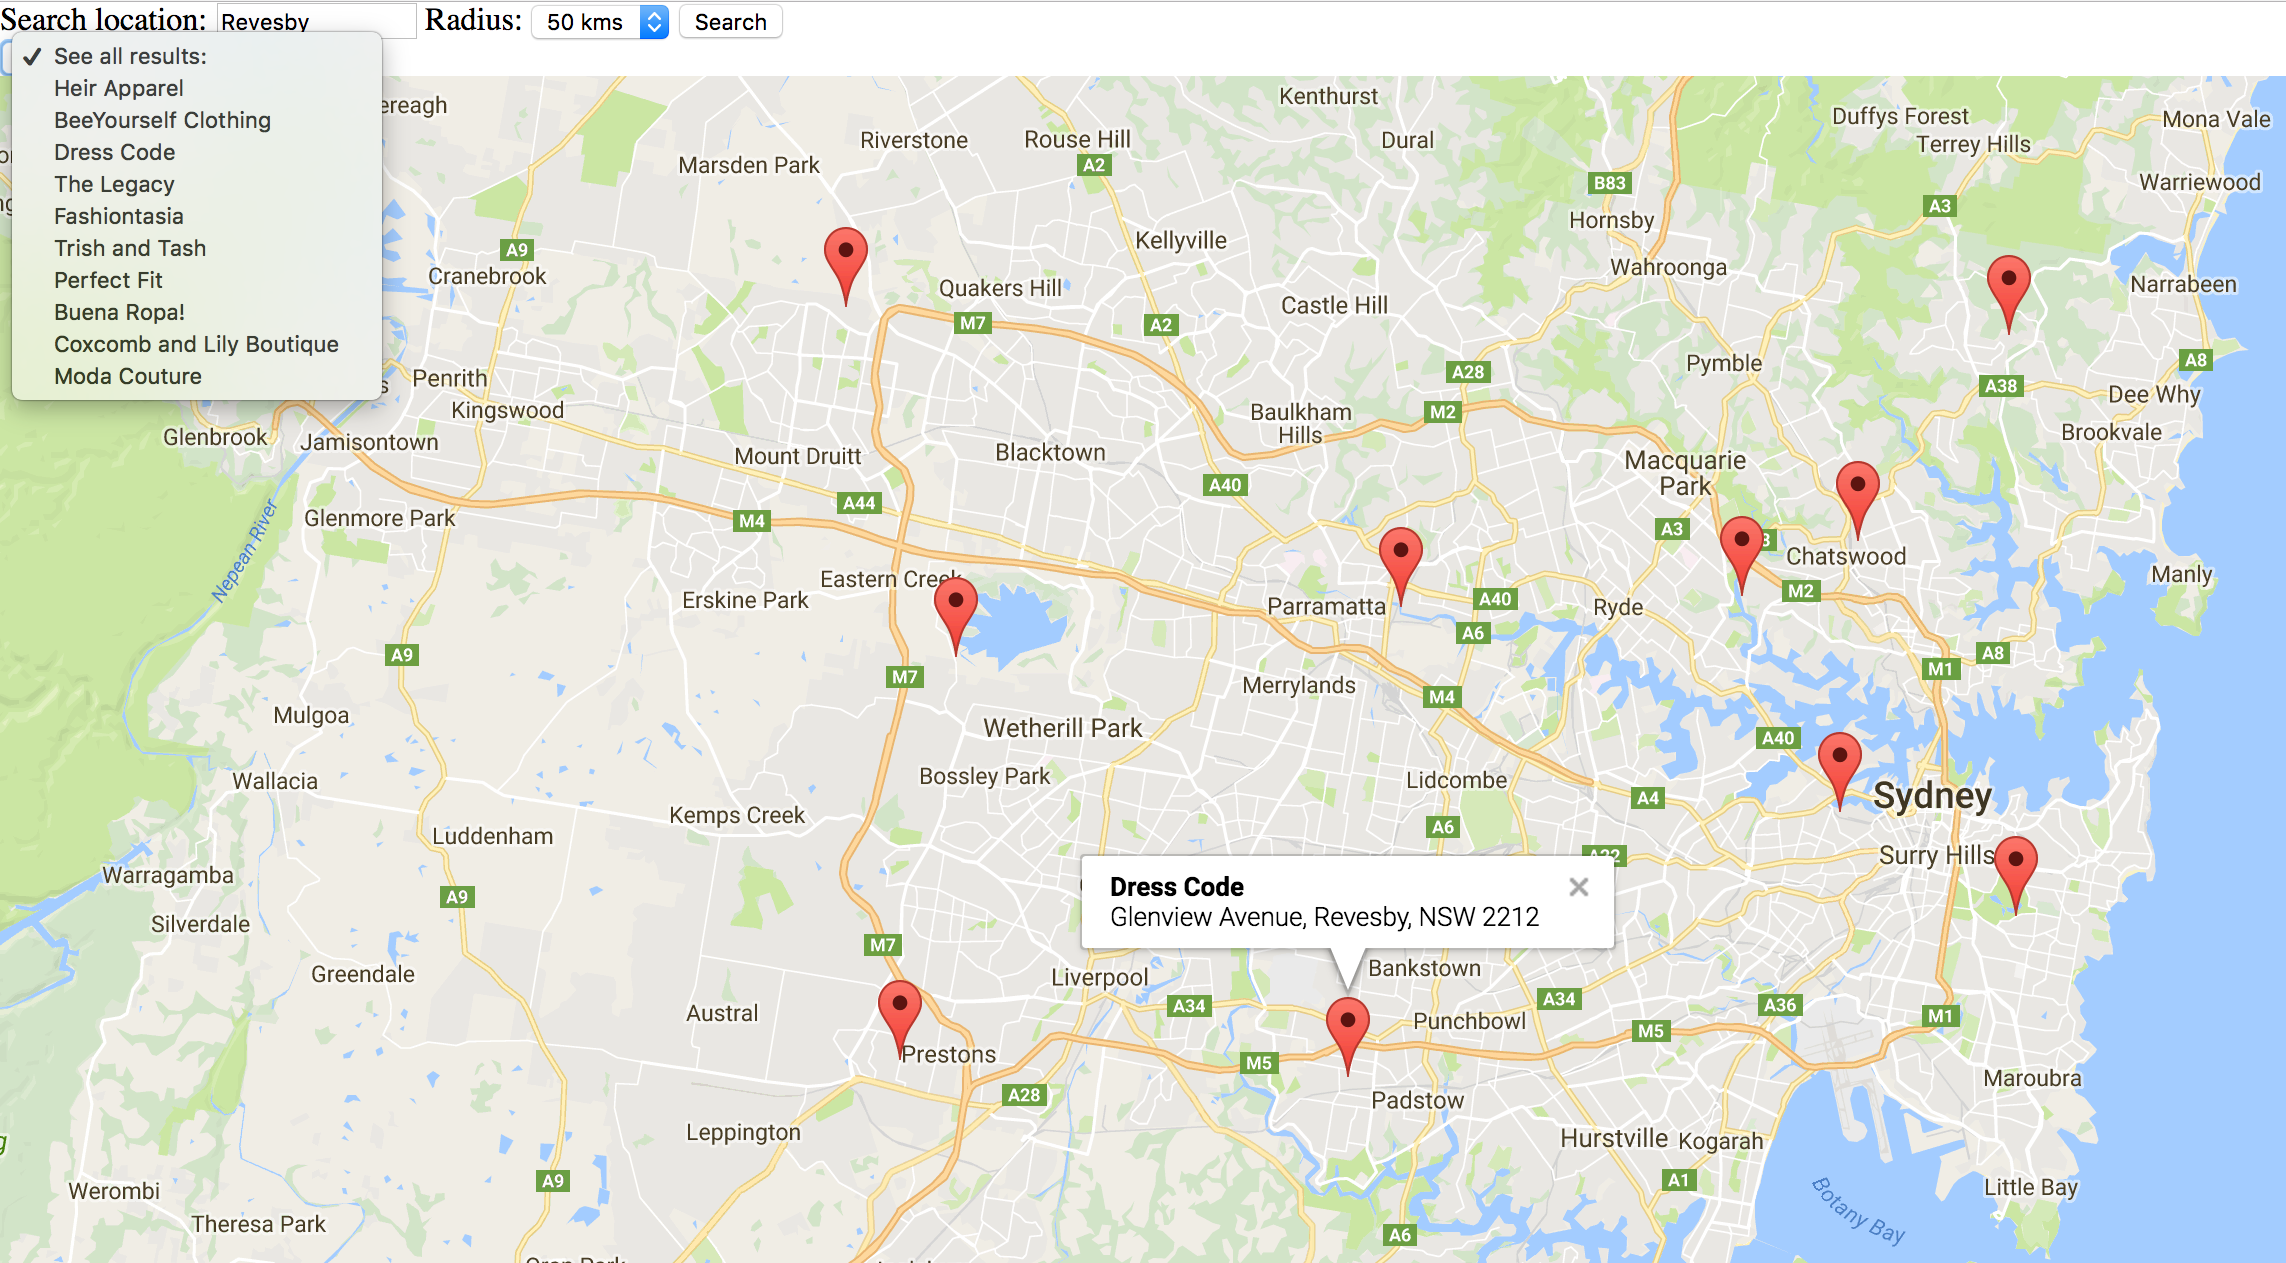
\includegraphics[scale=.17]{Capitulo2/images/geolocation}
	\caption{Ejemplo de uso de geolocalización a través del API de Google Maps}
	\label{fig:geolocation}
\end{figure}

Si una aplicación desea hacer uso de la geolocalización, esta deber ajustarse al estándar de Geolocalización de la W3C.

Dentro del estándar W3C, se definen los parámetros de información que pueden ser accedidos a partir del API Geolocation \citep{MarcoTeorico15}:
\begin{itemize}
	\item Accuracy: Representa la exactitud con la que fueron tomadas las últimas lecturas de la latitud y longitud del dispositivo con un 95\% de confianza.
	\item Altitude: Representa la cantidad en metros sobre la elipsoide WGS84.
	\item Altitude Accuracy: Representa la exactitud con la que fué tomada la última lectura de la altitud del dispositivo.
	\item Heading: Representa la dirección de desplazamiento en grados contando en el sentido de las agujas del reloj con respecto al norte verdadero en el rango de 0 <= rumbo <= 360.
	\item Latitude: Representa la coordenada de latitud de la geolocalización en grados decimales.
	\item Longitude: Representa la coordenada de longitud de la geolocalización en grados decimales.
	\item Speed: Representa la magnitud de la componente horizontal de la velocidad en metros por segundo.
\end{itemize}

 \paragraph{WGS84} El WGS84 (World Geodetic System 1984) es un sistema de coordenadas geográficas mundial que permite localizar cualquier punto de la Tierra (sin necesitar otro de referencia) por medio de tres unidades dadas (x,y,z). \citep{MarcoTeorico15}.

Se trata de un estándar en geodesia, cartografía, y navegación, que data de 1984. Tuvo varias revisiones (la última en 2004), y se considera válido hasta una próxima reunión (aún no definida en la página web oficial de la Agencia de Inteligencia Geoespacial). Se estima un error de cálculo menor a 2 cm, por lo que es en la que se basa el Sistema de Posicionamiento Global (GPS).

%%%%%%%%%%%%%%%%%%%%%%%%%%%%%%%%%%%%%%%%%%%%%%%%%%%%%%%%%%%%%%%%%%%%%%%%%
%           Capítulo 3: Análisis del Sistema
%%%%%%%%%%%%%%%%%%%%%%%%%%%%%%%%%%%%%%%%%%%%%%%%%%%%%%%%%%%%%%%%%%%%%%%%%
\chapter{Análisis del sistema}\label{chapter3}
\section{Factibilidad}
\subsection{Factibilidad técnica}
La factibilidad técnica de un proyecto estudia si el equipo y software existentes tienen las capacidades técnicas requeridas para que el proyecto resulte viable\cite{factibilidad_tecnica}.

En la Tabla \ref{tabla_factibilidad_tecnica}, se muestran los diferentes aspectos analizados para el desarrollo del presente trabajo.

\begin{longtable}{|M{3cm}|M{4cm}|M{2.5cm}|M{3cm}|M{1.5cm}|}
	\hline
	\textbf{Problemática} & \textbf{Solución propuesta} & \textbf{Tiempo de desarrollo} & \textbf{Precio estimado} & \textbf{¿Resulta factible?} \\ \hline
	Necesidad de medir la cantidad de combustible& Uso de un caudalímetro (véase la sección \ref{sec:Sensor}) & No aplica, se adquiere desarrollado & Aproximadamente \$500 & Si\\\hline
	Necesidad de enviar las mediciones registradas por el sensor & Uso de un microcontrolador (véase la sección \ref{sec:micro}) & No aplica, se adquiere desarrollado & Aproximadamente \$200 & Si\\\hline
	Enviar las mediciones registradas a un dispositivo móvil inalambricamente & Uso de módulo Bluetooth (véase la sección \ref{sec:bluetooth}) & N/A, se adquiere desarrollado & Aproximadamente \$100 & Si \\\hline
	Desarrollar un aplicación para un dispositivo móvil Android & Usar el lenguaje de programación Java y el IDE Android Studio para el desarrollo de un aplicación compatible con teléfonos Android 5+& 6 meses & No aplica, tanto el uso de Java como de Android Studio es gratuito & Si \\ \hline
	Desarrollar un servidor web al cual pueda conectarse la aplicación móvil & Usar el framework web Java Spring 4 y el IDE Eclipse para el desarrollo& 6 meses & No aplica, Spring 4 y Eclipse son gratuitos & Si \\ \hline
	Desplegar el servidor web sobre un servicio de cloud computing  & Usar un servicio de cloud computing como Google Cloud & 1 mes & Aproximadamente \$1000/año & Si \\ \hline
	Programar el microcontrolador para recibir y enviar las mediciones & Usar lenguaje C y Atmel Studio para programar el microcontrolador & 3 meses & N/A, Atmel Studio es gratuito & Si \\ \hline
	\caption{Factibilidad técnica}
	\label{tabla_factibilidad_tecnica} 
\end{longtable}
\subsection{Factibilidad operativa}
La factibilidad operativa tiene como objetivo comprobar que la empresa u organización será capaz de darle uso al sistema, que cuenta con el personal capacitado para hacerlo o tiene los recursos humanos necesarios para mantener el sistema\cite{factOperativa}.
\\
Para saber si el producto es factible operativamente o no, es necesario conocer los indices de aprobación del sistema entre los habitantes de la Ciudad de México; para conocer dicho parámetro se realizó una encuesta a una parte de la población, obteniendo que el sistema impacta de forma positiva a más de la mitad de la población encuestada, siendo una herramienta de utilidad para los mismos.
\\
Con la finalidad de garantizar el buen funcionamiento y uso del sistema, se planteo realizar la aplicación en Android, contando con la aprobación de los usuarios encuestados en su mayoría.
\\
La necesidad de los usuarios por conocer cuales son las gasolineras que mejor despachan la gasolina, lleva a la aceptación de la aplicación móvil ya que brinda una solución a su necesidad, ademas de que por su practicidad y su facilidad de operación lleva a que el sistema sea factible operativamente.
\\
Para conocer a detalle los resultados de la encuesta revisar el Apéndice B.
%Lo que teniamos antes
\begin{comment}
En la Tabla \ref{tabla_factibilidad_operativa}, se muestran los diferentes aspectos analizados para el desarrollo del presente trabajo.

\begin{longtable}{|M{2.5cm}|M{3cm}|M{2cm}|M{2cm}|M{2cm}|M{2cm}|}
	%\centering
		\hline
		\textbf{Personal} & \textbf{Actividades} & \textbf{Salario Mensual} & \textbf{Cantidad de Personas} & \textbf{Tiempo} & \textbf{Salario total por desarrollo} \\ \hline
		Programador Android &
		Desarrollo de la aplicación móvil.
		 & \$8 000 & 1 & 6 meses &  \$48 000 \\\hline
		Administrador de base de datos & Diseño e implementación de la base de datos & \$8 000 & 1 & 6 meses  & \$48 000 \\\hline
		Ing. en sistemas computacionales & 
		\begin{itemize}
			\item Análisis y diseño del servidor web
			\item Desarrollo del hardware del proyecto
		\end{itemize}
		& \$8 000 & 1 & 6 meses & \$48 000 \\ \hline
		\multicolumn{5}{|r|}{Total} & \$144 000 \\ \hline
	\caption{Factibilidad operativa}
	\label{tabla_factibilidad_operativa} 
\end{longtable}
\end{comment}
\subsection{Factibilidad económica}
La siguiente sección presenta la factibilidad económica del proyecto, ésta se encuentra divida en tres partes donde se realiza el análisis económico del módulo de hardware, posteriormente se realiza el análisis y las estimaciones del módulo de software, y finalmente se calcula el costo total del proyecto realizando un análisis de la factibilidad del proyecto.

\subsubsection{Hardware}
La estimación de Hardware, se realizará con base en los componentes electrónicos que integrarán cada unidad de medición que se venderá al usuario final, dicha unidad de medición deberá cumplir con las siguientes características:
\begin{itemize}
	\item Permitirá la medición de la cantidad de litros ingresados a un automóvil durante el proceso de suministro de gasolina.
	\item Permitirá la comunicación entre el sensor y una aplicación móvil.
\end{itemize}

\paragraph{Unidad de medición} Para cumplir con las características se hará uso de los siguientes elementos de hardware:

\begin{longtable}{|M{4cm}|M{6.5cm}|M{4cm}|}
	\hline
	\textbf{Unidad de hardware} & \textbf{Descripción} &\textbf{Valor (MXN)}
	\\\hline
	Caudalimetro Modelo FS400A-G1 & Permite la medición de la cantidad de litros de gasolina que pasan a través del sensor & \$348
	\\\hline
	Microcontrolador Modelo ATmega16 & Permite el tratamiento y el análisis de la señal generada por el caudalímetro & \$100
	\\\hline
	Modulo Bluetooth Modelo Hc-06  & 8~60 litros/min & \$145
	\\\hline
	\caption{Estimaciones de costos para el modulo de hardware}
	\label{tabla_fatibilidad_economica} 
\end{longtable}
A continuación, se ponen las URL de los sitios web donde se compraron los componentes, puede dar click en el componente deseado y será redirigido a la página web correspondiente:

\begin{itemize}
	\item  \href{https://articulo.mercadolibre.com.mx/MLM-563607650-caudalimetro-sensor-de-flujo-liquidos-1-pulgada-1-a-60-lmin-_JM?fbclid=IwAR1_qJeWVCpg_5bPhjg7R-Mcx2q9eO3CDDKzBXMvJtp12USAU0zp46vphmk}{Caudalímetro}
	\item \href{https://articulo.mercadolibre.com.mx/MLM-552397250-modulo-bluetooth-hc-06-para-arduino-pic-raspberry-_JM?matt_tool=&matt_word=&gclid=CjwKCAjw9sreBRBAEiwARroYm1LdtLoloDq74O455SEt5xQutPzGfCwV67LSzx-MMpatIKUnfq6yphoCuKMQAvD_BwE}{Microcontrolador}
	\item \href{https://www.microchip.com/wwwproducts/en/ATmega16}{Módulo Bluetooth} 
\end{itemize}

\paragraph{Precio unitaria por unidad de medición}La tabla anterior nos arroja que cada unidad de medición de producción creada necesitará una inversión mínima de \$629 para obtener todos sus componentes. Esta medida unitaria será sumada a las estimaciones de software para poder realizar el posterior análisis de factibilidad.


\subsubsection{Software}
Para el análisis de costos de software, así como para las estimaciones se utilizaron las siguientes herramientas:
\begin{itemize}
	\item Estimación del costo del proyecto: Modelo COCOMO II
	\item Estimación de la demanda: Benchmarking, Técnicas de recolección de Información (encuestas).
\end{itemize}


\paragraph{Estimaciones del proyecto}
Comenzaremos la estimación del proyecto identificando los componentes de software que conformarán el Trabajo Terminal, el análisis actual contempla los siguientes componentes: Servidor Web, Base de Datos y la Aplicación Móvil.

Una vez que se han definido componentes de software del proyecto se describirán los factores y las técnicas utilizadas para la estimación del costo del proyecto.

\paragraph{Métricas} Es importante definir algunos puntos importantes que influyen en nuestra estimación de costos.
\begin{itemize}
	\item Complejidad: Elevada, debido a la integración de diferentes de hardware y software.
	\item Tamaño: Medio, debido a la cantidad de módulos y submódulos a desarrollar tanto de hardware como software
	\item Grado de Incertidumbre: Medio, debido a la experiencia del equipo.
	\item Disponibilidad de Información Histórica: Elevado, debido a la cantidad de proyectos similares a los cuáles se tiene acceso.
\end{itemize}

Para éste proyecto se desarrollaron las estimaciones de: 
\begin{itemize}
	\item Costo – Medido en MXN.
	\item Esfuerzo – Medido en Personas/Mes
	\item Tiempo – Medido en meses
\end{itemize}	

utilizando dos técnicas de Ingeniería de Software, enumeradas a continuación:

\begin{itemize}
	\item Técnicas de Descomposición: Específicamente se hizo uso de Estimaciones por número de LOC
	\item Técnicas Empíricas: Mediante el uso del Modelo COCOMO II
\end{itemize}
\paragraph{Estimación por el Modelo COCOMO II}
El primer paso para la estimación por modelo COCOMO es la obtención de la Métrica de Software conocida como LOC Lines Of Code, la cual, representa el número de líneas de código que se escribieron para poder liberar una funcionalidad dentro del sistema.
A continuación, se muestra una tabla en la que se enumeran los LOC para cada módulo y sus correspondientes submódulos del proyecto.



\subsection{Análisis de factibilidad}
De acuerdo con los parámetros obtenidos en la métricas de hardware y software se realiza el siguiente análisis de factibilidad económica:
\begin{itemize}
	\item En fase de desarrollo el proyecto terminal resulta viable pues los elementos de hardware necesarios tiene  un precio de aproximadamente \$500, las demás herramientas de software, pruebas, así como la mano de obra son proporcionadas por el IPN y los integrantes del equipo.
	\item Por otro lado si el actual proyecto llegará la etapa de comercialización, los costos unitarios por la producción de cada unidad de medición aumentarían y los costos de desarrollo de software deberían ser cubiertos mediante el uso de un crédito, lo cuál nos llevaría a establecer un análisis de la demanda saber si la TIR (Tasa de Retorno de Inversió) es favorable.
\end{itemize}
\section{Requerimientos funcionales}
A continuación, se presenta un listado con los requerimientos funcionales que se obtuvieron.
El listado de requerimientos funcionales se encuentra divido de acuerdo con los submódulos que se identificaron:
\begin{itemize}
	\item Submódulo de Uusarios.
	\item Submódulo de Mediciones.
	\item Submódulo de Clasificación.
\end{itemize}

\paragraph{Submódulo de Usuarios}
\begin{enumerate}[label=RF\arabic*.]
	\item Proporcionar una interfaz que permita registrar, editar, consultar y eliminar los datos personales de un usuario en la plataforma.
	\item Proporcionar un mecanismo de autenticación para el usuario.
	\item Proporcionar un mecanismo de recuperación de credenciales para el usuario.
	\item Proporcionar una interfaz que permita, registrar, editar, consultar y eliminar los automóviles de un usuario.
	\item Asociar un caudalímetro con un automóvil para una medición.
	\item Proporcionar un mecanismo para la generación de reportes de problemas con el sensor o la aplicación.
	\item Consultar las mediciones realizadas por el usuario.
	\item Proporcionar un mecanismo para la geolocalización de un usuario a través de un dispositivo móvil.
	\item Proporcionar un mecanismo de obtención de los datos de las gasolineras cercanas a un usuario, según su geolocalización.
	\item Proporcionar un mecanismo para la asignación de insignias a un usuario.
	\item Consultar las insignias obtenidas por el usuario.
	\item Compartir las mediciones o insignias obtenidas en redes sociales.
\end{enumerate}

\paragraph{Submódulo de Mediciones}
\begin{enumerate}[label=RF\arabic*.]
	\setcounter{enumi}{12}
	\item Proporcionar una interfaz para registrar los datos usados por el usuario durante el suministro de gasolina como, la cantidad de litros de gasolina cargados y el precio por litro.
	\item Proporcionar un dispositivo electrónico que permita la medición de los litros de gasolina ingresados al automóvil.
	\item Proporcionar un mecanismo que permita la comunicación vía Bluetooth entre el dispositivo electrónico y una aplicación móvil,
	\item Proporcionar un mecanismo que permita la comunicación vía HTTP entre una aplicación móvil y un servidor que reciba los datos de las mediciones recabadas por el dispositivo electrónico.
\end{enumerate}

\paragraph{Submódulo de Clasificación}
\begin{enumerate}[label=RF\arabic*.]
	\setcounter{enumi}{16}
	\item Proporcionar un algoritmo para la clasificación de las gasolineras de acuerdo con las mediciones recabadas.
	\item Proporcionar un mecanismo para el registro, edición, consulta y eliminación de los datos de una gasolinera.
	\item Proporcionar un mecanismo para la asignación de insignias a una gasolinera.
	\item Consultar las insignias obtenidas por una gasolinera.
\end{enumerate}
\section{Requerimientos no funcionales}\label{RequerimientosNF}
A continuación, se presenta un listado con los requerimientos no funcionales que fueron identificados para el sistema:
\begin{enumerate}[label=RNF\arabic*.]
	\item Escalabilidad: La arquitectura bajo la que es construido el sistema permite que este sea escalable y pueda extenderse hacia más usuarios y más funcionalidades.
	\item Seguridad: Todos los usuarios que se registren deberán de activar sus cuentas vía correo electrónico.
	\item Usabilidad: La interfaz de usuario del sistema es intuitiva de tal forma que un usuario pueda usar las funcionalidades descritas en los requerimientos funcionales, sin entrenamiento previo en no más de dos horas.
	\item Tiempo de ejecución: Cuando se envíe una petición al servidor para mostrar la información de la clasificación de las gasolineras este debe responder en un tiempo máximo de 5 segundos.
	\item Tolerancia a fallos: Cuando se presente un error en el sistema, este no tardará más de 5 minutos en restaurarse a un estado válido.
	\item Concurrencia: El sistema debe soportar 1000 peticiones sin que el tiempo de respuesta para todas ellas sea mayor a 10 segundos.
\end{enumerate}
\section{Requerimientos técnicos}
Para utilizar el sistema es necesario que los usuarios cuenten con ciertos requisitos en sus teléfonos móviles, dichos requisitos se enunciaran a continuación.
\subsection{Requerimientos mínimos de software}
\begin{enumerate}
	\item Sistema Operativo:Android 5.0 o superior.
\end{enumerate}
\subsection{Requerimientos mínimos de hardware}
\begin{enumerate}
	\item Memoria RAM: 2GB
	\item Almacenamiento: Espacio libre mayor a 150 MB.
	\item Comunicación inalambrica: Bluetooth version 4.1
	\item Procesador: Dual-Core de 1.2 GHz
\end{enumerate}
\section{Reglas de negocio}
En la presente sección, se muestran las reglas de negocio del sistema.
\begin{enumerate}[label=RN\arabic*.]
	\item \label{RN1}
		\begin{description}
			\item[Nombre] RN1-Calcular cantidad de combustible recargado.
			\item[Tipo] Derivadora.
			\item[Objetivo] La cantidad de combustible recargado a un automóvil se calcula con una fórmula especifica dependiente del sensor de hardware usado.
			\item[Descripción] La cantidad de combustible recargado a un automóvil, se calcula con la fórmula: $$L=(F/4.8)*T$$
			Donde:
				\begin{itemize}
					\item L=Total de litros recargados
					\item F=Frecuencia de la señal (tren de impulsos) enviada por el sensor de hardware, se calcula por la cantidad de impulsos (voltaje en alta) que se reciban en un segundo.
					\item T= Es el tiempo durante el que se recibió la señal, el tiempo se calcula al establecer una marca de tiempo en la cual se recibió el primer impulso, y establecer otra marca de tiempo en el momento en que se han dejado de recibir. Restando al segundo el primero.\cite{FS400A-G1}
				\end{itemize}
			% \item[Ejemplo]
		\end{description}

	\item \label{RN2}
		\begin{description}
			\item[Nombre] RN2-Tiempo posterior a la carga de combustible.
			\item[Tipo] Controladora.
			\item[Objetivo] Especificar la cantidad de tiempo, en la que pasado este se considera que la recarga de combustible en el automóvil haya culminado.
			\item[Descripción] Se considera que se ha dejado de cargar gasolina a un automóvil sí ha pasado más de diez segundos sin recibir una trama con un valor distinto a cero.
			% \item[Ejemplo]
		\end{description}
	\item \label{RN3}
		\begin{description}
			\item[Nombre] RN3-Otorgar insignia a actor.
			\item[Tipo] Derivadora.
			\item[Objetivo] Determinar las condiciones bajo las cuales un actor recibe una insignia.
			\item[Descripción] Un actor recibe una insignia cada vez que acumula cien mediciones.
			% \item[Ejemplo]
		\end{description}
	\item \label{RN4}
		\begin{description}
			\item[Nombre] RN4-Registrar precio gasolina.
			\item[Tipo] Controladora.
			\item[Objetivo] Determinar que actores pueden registrar el precio de la gasolina después de haber cargado.
			\item[Descripción] Solamente un actor con insignias puede registrar el precio de la gasolina.
			% \item[Ejemplo]
		\end{description}
	\item \label{RN5}
		\begin{description}
			\item[Nombre] RN5-Asignar insignia a gasolinera.
			\item[Tipo] Controladora.
			\item[Objetivo] Determinar que actores pueden asignarle una insignia a una gasolinera.
			\item[Descripción] Solamente un actor con insignias puede asignarle insignias a una gasolinera después de carga gasolina en la misma.
			% \item[Ejemplo]
		\end{description}
	\item \label{RN6}
		\begin{description}
			\item[Nombre] RN6-Especificar bomba.
			\item[Tipo] Controladora.
			\item[Objetivo] Determinar que actores pueden especificar en que bomba cargaron gasolina.
			\item[Descripción] Solamente un actor con al menos una insignia puede especificar en que bomba cargó gasolina.
			% \item[Ejemplo]
		\end{description}
	\item \label{RN7}
		\begin{description}
			\item[Nombre] RN7-Actualizar clasificación de gasolineras.
			\item[Tipo] Controladora.
			\item[Objetivo] Determinar el tiempo que debe pasar entre cada actualización de la clasificación de gasolineras.
			\item[Descripción] La clasificación de gasolineras se actualiza cada veinticuatro horas.
			% \item[Ejemplo]
		\end{description}
	\item \label{RN8}
		\begin{description}
			\item[Nombre] RN8-Radio cercano al actor para obtener gasolineras.
			\item[Tipo] Derivadora.
			\item[Objetivo] Especificar en que radio se obtendrán las gasolineras cercanas al actor al abrir la aplicación móvil.
			\item[Descripción] El radio es de quinientos metros a partir de la ubicación del actor.
			% \item[Ejemplo]
		\end{description}
	\item \label{RN9}
		\begin{description}
			\item[Nombre] RN9-Iconos de gasolineras.
			\item[Tipo] Derivadora.
			\item[Objetivo] Especificar que tipo de icono se mostrará según el tipo de gasolinera obtenida.
			\item[Descripción] Las gasolineras registradas en el sistema se mostrarán de color negro con un tamaño de 24 pixeles. Las gasolineras que únicamente se encuentren en el API de Google Maps se mostrarán de color rojo en un tamaño de 12 pixeles.
			% \item[Ejemplo]
		\end{description}
	\item \label{RN10}
		\begin{description}
			\item[Nombre] RN10-Verificar cuenta de usuario.
			\item[Tipo] Controladora.
			\item[Objetivo] Controlar las acciones que puede realizar un usuario sin una cuenta verificada.
			\item[Descripción] Un usuario que aún no haya verificado su cuenta, puede realizar las mismas acciones que un usuario no registrado, hasta que verifique su cuenta.
			% \item[Ejemplo]
		\end{description}
	\item \label{RN11}
		\begin{description}
			\item[Nombre] RN11-Consistencia de información.
			\item[Tipo] Derivadora.
			\item[Objetivo] Verificar que la información ingresada por un usuario sea válida respecto a lo establecido en la presente regla de negocio.
			\item[Descripción] La información ingresada por un usuario en un formulario, no puede ser igual a la cadena vacía ``'', a excepción de que sea un campo no obligatorio.
			% \item[Ejemplo]
		\end{description}
	\item \label{RN12}
		\begin{description}
			\item[Nombre] RN12-Cuenta no verificada.
			\item[Tipo] Derivadora.
			\item[Objetivo] Verificar que un usuario al iniciar sesión tenga su cuenta activa.
			\item[Descripción] Un usuario no puede autenticarse en el sistema en caso de que no tenga una cuenta activa, por lo cual deberá ser notificado para que verifique su cuenta, así como tampoco puede solicitar recuperar su contraseña.
			% \item[Ejemplo]
		\end{description}
\end{enumerate}
\section{Análisis de riesgos}
El análisis de los riesgos del presente Trabajo Terminal, nos permite identificar cuales son los factores de riesgo, que potencialmente tienen un impacto negativo en el mismo. Por lo cual, es necesario prestar atención a estos. Una vez identificados y clasificados los riesgos, es posible realizar un análisis de los mismos, con la finalidad de encontrar soluciones u métodos que nos permitan solventar los mismos \cite{RIESGO}, en la Tabla \ref{tabla_riesgos} se muestra un listado de los mismos.\\
\begin{longtable}{|M{3cm}|M{2cm}|M{3.8cm}|M{5.5cm}|}
	% \centering
	% \begin{tabular}
	\hline
	\textbf{Área de impacto} & \textbf{Nivel de impacto} & \textbf{Causas} & \textbf{Métodos para contrarrestar el riesgo} \\ \hline
	Modificación de los requerimientos funcionales & Alto & No haber contemplado dentro del análisis funcionalidades importantes. & Evaluar al termino de cada incremento, si los resultados obtenidos van acorde con lo definido en los requerimientos funcionales y los objetivos. \\ \hline
	Atraso en fechas de entrega & Alto & 
	No tener listas las actividades especificadas en los cronogramas.
	& Evaluar al termino de cada mes, si se cumplieron las actividades esperadas y en caso negativo, analizar el porque y justificarlo en el anexo correspondiente (\ref{anexo:atraso}). \\ \hline
	Hardware & Alto &
	\begin{itemize}
		\item Sensor de flujo defectuoso o no adecuado.
		\item Incompatibilidad del sensor con el microcontrolador.
		\item Fallas en la comunicación inalámbrica entre el microcontrolador y el dispositivo móvil.
		\item Dispositivo móvil sin capacidades de conexión inalámbrica.
		\item Cortos circuitos.
		\item Batería que alimenta el circuito del sensor descargada.
	\end{itemize} &
	\begin{itemize}
		\item Realizar una comparación de diversos sensores para posteriormente realizar pruebas con alguno de ellos, y verificar así su funcionalidad.
		\item Elegir el microcontrolador a partir del sensor seleccionado y no de forma inversa.
		\item Seleccionar un dispositivo de comunicación inalámbrica adecuado para el microcontrolador seleccionado y realizar pruebas de comunicación.
		\item Notificar al usuario que para poder usar la aplicación es necesario que tenga un dispositivo móvil el cual cumpla con ciertas condiciones de hardware y software.
		\item Realizar extensivas pruebas para verificar que el diseño del sensor evite cortos circuitos.
		\item Realizar una implementación de hardware la cual permita recargar la batería que alimenta el circuito.
	\end{itemize} \\ \hline
	Software & Medio &
	\begin{itemize}
		\item Software que no permite la escalabilidad.
		\item Uso de tecnología obsoletas o que estén próximas a quedar obsoletas.
	\end{itemize} &
	\begin{itemize}
		\item Usar una arquitectura que permita que el sistema sea escalable.
		\item Seleccionar una tecnología que sea un estándar en la industria.
	\end{itemize} \\ \hline
	Reputación y confianza del usuario & Alto &
	\begin{itemize}
		\item Desconfianza de que la información mostrada en la aplicación sea errónea.
		\item Producto que no funcione de la manera esperada.
	\end{itemize} &
	\begin{itemize}
		\item Realizar mediciones precisas bajo el margen establecido en la norma NOM-005-SCFI-2011\cite{NORMA-005}.
		\item Probar continuamente los diversos incrementos que se realizan sobre el equipo de hardware y el software.
	\end{itemize}
	\\ \hline
	% \end{tabular}
	\caption{Análisis de Riesgos}
	\label{tabla_riesgos}
\end{longtable}
\section{Descripción del software}
\subsection{Android}
Es un sistema operativo móvil desarrollado por Google; está basado en Linux, que junto con aplicaciones middleware está enfocado para ser utilizado en dispositivos móviles como teléfonos inteligentes, tables, Google TV y otros dispositivos.
A continuación, en la Tabla \ref{Tabla_android} se muestra una comparación entre distintos sistemas operativos para dispositivos móviles.
\begin{table}[H]
	\centering
	\begin{tabular}{|M{3.2cm}|M{3cm}|M{3cm}|M{3cm}|}
		\hline 
		\textbf{Características} & \textbf{Android} & \textbf{IOS} & \textbf{Windows Phone} \\ \hline
		Núcleo & Linux & XNU & Windows NT \\ \hline
		Arquitectura soportada & ARM, MIPS, x86 & ARM & ARM, Microsoft XNA \\ \hline
		Programado & C, C++ y Java & C, C++, Objective-c y Swift & XNA, NET, C\#, C, C++ y VB.NET \\ \hline
		Entorno de desarrollo & Android Studio & Xcode & Visual Basic \\ \hline
		Conectividad & GSM/EDGE, IDEN, CDMA, EV-DO, UMTS, Bluetooth, WiFi, LITE, HSDPA, HSPA+, NFC y WiMAX & WiFi.802.11AC, Bluetooth LE & WiFi 802.11b/g y Bluetooth \\ \hline
		Sincronización con la nube & Google Drive & iCloud & SkyDrive \\ \hline
		Tienda de aplicaciones & Google Play & App Store & Windows Phone Store \\ \hline
		Almacenamiento de datos & SQLite & SQLite & SQLite \\ \hline
		Navegador web & Chrome & Safari & Internet Explorer \\ \hline
		Tipo de interfaz & Iconos y widgets & Iconos & Baldosas animadas \\ \hline
	\end{tabular}
	\caption{Tabla comparativa de dispositivos móviles}
	\label{Tabla_android}
\end{table}

Al comprar las características de las distintas tecnologías para dispositivos móviles, se decidió utilizar Android debido a que existe una gran parte de la población que cuenta con un dispositivo con este sistema operativo, asimismo nos brinda mayores posibilidades de conectividad y un entorno de desarrollo más accesible debido a que es una tecnología OpenSource.


\subsection{Java}
Java es un lenguaje de programación y una plataforma informática comercializada por primera vez en 1995 por Sun Microsystems.\\
Es una tecnología que se usa para el desarrollo de aplicaciones que convierten a la Web en un elemento más interesante y útil.
Java permite jugar, cargar fotografías, chatear en línea, realizar visitas virtuales y utilizar servicios como, por ejemplo, cursos en línea, servicios bancarios en línea y mapas interactivos \citep{java}.
En la tabla \ref{tabla_lenguajes} se muestra una tabla comparativa entre tres distintos lenguajes de programación.
\begin{longtable}{|M{2.5cm}|M{3cm}|M{4.2cm}|M{4.3cm}|}
		\hline 
		\textbf{Lenguaje} & \textbf{Características} & \textbf{Ventajas} & \textbf{Desventajas} \\ \hline
		Java & Lenguaje orientado a objetos & \begin{itemize}
			\item Multiplataforma
			\item No existen problemas con la liberación de la memoria en el sistema.
			\item Cuenta con una amplia variedad de bibliotecas estándar.
		\end{itemize} &  \begin{itemize}
		\item Tiene un rendimiento menor comparado con los demas lenguajes de programación.
		\item Es necesario tener la maquina virtual de Java para poder ejecutar los programas.
		\item Es un lenguaje que evoluciona muy lentamente
	\end{itemize} \\ \hline
		C\# & Lenguaje de programación orientado a objetos & \begin{itemize}
			\item Declaración en el espacio de nombres
			\item Existe un rango más amplio y definido de tipos de datos.
			\item Propiedades: un objeto tiene intrínsecamente propiedades.
		\end{itemize} & \begin{itemize}
		\item Se necesita una versión reciente de VS.NET
		\item Se requiere Windows NT 4 o superior
	\end{itemize} \\ \hline
		Python & Lenguaje de programación interpretado y orientado a objetos & \begin{itemize}
			\item Tipado dinamico
			\item Facilidad de aprendizaje
			\item Sintaxis sencilla
		\end{itemize} & \begin{itemize}
		\item Al ser un lenguaje interpretado lo vuelve mas lento.
	\end{itemize} \\ \hline
	\caption{Tabla comparativa de diferentes lenguajes de programación}
	\label{tabla_lenguajes}
\end{longtable}
El lenguaje de programación que será utilizado en el presente proyecto será Java, debido a que el desarrollo de aplicaciónes moviles y web es mas sencillo. Ademas Java nos da la posibilidad de compilar una sola vez el proyecto y poder ejecutarlo en cualquier plataforma sin tener que recompilarlo de nuevo. Asimismo Java nos brinda seguridad, portabilidad y fiabilidad.
\subsection{Spring 4}
Spring Framework proporciona un completo modelo de programación y configuración para aplicaciones empresariales modernas basadas en Java, en cualquier tipo de plataforma de implementación.
Un elemento clave de Spring es el soporte de infraestructura en el nivel de la aplicación: Spring se centra en la "plomería" de las aplicaciones empresariales para que los equipos puedan enfocarse en la lógica empresarial a nivel de la aplicación, sin vínculos innecesarios con entornos de implementación específicos \citep{spring}.
\\
En la tabla \ref{tabla_frameworks} se muestra una tabla comparativa entre distintos frameworks.
\begin{longtable}{|M{3cm}|M{4.2cm}|M{4.2cm}|M{4.3cm}|}
	\hline 
	\textbf{Framework} & \textbf{Ventajas} & \textbf{Desventajas} \\ \hline
	Spring 4 & \begin{itemize}
		\item Lenguaje Java
		\item Fácil configuración
		\item Open source
		\item Estandarizado
	\end{itemize} &  \begin{itemize}
		\item Te atrae a que te adaptes al sistema.
	\end{itemize} \\ \hline
	Django & \begin{itemize}
		\item Desarrollo rápido
		\item Open source
		\item Fácil de aprender
		\item MVT
	\end{itemize} & \begin{itemize}
		\item Templates no tan robustos
		\item Se reinicia el servidor al recargar
		\item ORM no tan robusto
	\end{itemize} \\ \hline
	Node.js & \begin{itemize}
		\item Javascript
		\item High-performance
		\item Open source
		\item Asíncrono
	\end{itemize} & \begin{itemize}
		\item Limitado a una CPU
	\end{itemize} \\ \hline
	\caption{Tabla comparativa de diferentes frameworks}
	\label{tabla_frameworks}
\end{longtable}
Se eligió spring 4 como el framework para el desarrollo de la lógica del servidor, debido a que nos ofrece la posibilidad de utilizar el lenguaje Java, previamente elegido como lenguaje de programación del sistema, y nos brinda un soporte robusto de aplicaciones lo cual nos permite que el sistema funcione correctamente aun si este mismo crece.
\subsection{Servidor}
Un servidor es un ordenador u otro tipo de equipo informático encargado de suministrar información a una serie de clientes, que pueden ser tanto personas como otros dispositivos conectados a él. La información que puede transmitir es múltiple y variada: desde archivos de texto, imagen o vídeo y hasta programas informáticos, bases de datos, etc.
\textbf{Cloud Server}
Los cloud servers son unas alternativas para llevar la herramienta de los servidores al mundo virtual. La infraestructura en la nube se consigue gracias a la existencia de diversos servidores físicos controlados mediante un software, que es el encargado de virtualizar la plataforma.
\\Los servidores en la nube ofrecen a las empresas la posibilidad de tener un servidor a medida de sus necesidades, cuyos recursos y capacidades puedan ir incrementándose a conforme aumentan el tamaño y la actividad de la empresa, lo que permite un considerable ahorro para el presupuesto de las distintas corporaciones \citep{servidores}.
\\
En la tabla \ref{tabla_servidores} se tiene la comparación entre distintos cloud servers.
\begin{longtable}{|M{2.5cm}|M{4cm}|M{4.8cm}|M{3cm}|}
	\hline 
	\textbf{Cloud Server}& \textbf{Descripción} & \textbf{Características} & \textbf{Precio} \\ \hline
	Google Cloud Platform & Es una plataforma que ha reunido todas las aplicaciones de desarrollo web de Google. Google Cloud Platform es utilizada para crear soluciones a través de la tecnología almacenadas en la nube. &\begin{itemize}
		\item Permite la conexión por medio de SSH.
		\item Puedes desplegar el código directamente o mediante contenedores.
		\item Solo se paga por el tiempo utilizado.
		\item Maquinas virtuales personalizadas.
		\item Cuenta con un almacenamiento de hasta 624 GB por maquina.
		\item Proporciona almacenamiento en bloques en unidades de estado solido locales con encriptado permanente.
		\item Balanceo de carga global.
		\item Sistemas operativos: Debian, CentOS, CoreOS, SUSE, Ubuntu, Red Hat, FreeBSD o Windows 2008 R2, 2012 R2 y 2016
		\item Procesamiento por lotes.
	\end{itemize} &  Aproximadamente 0.1900 USD/hora \\ \hline
	Amazon Web Services & 
	Es una plataforma de servicios de nube que ofrece potencia de cómputo, almacenamiento de bases de datos, entrega de contenido y otra funcionalidad para ayudar a las empresas a escalar y crecer.
	&\begin{itemize}
		\item Instancias dedicadas: brindan acceso directo al procesador y a la memoria del servidor.
		\item Instancias de informática con GPU
		\item Instancias de E/S de alto desempeño: Ofrecen un desempeño de disco secuencia de hasta 16 GB/s
		\item Instancias de almacenamiento denso: Hasta 48 TB de almacenamiento.
		\item Volúmenes de almacenamiento en bloques persistente, de alta disponibilidad, constantes y de baja latencia
		\item Se paga por lo que se consuma
		\item Posibilidad de colocar las instancias en distintas ubicaciones.
		\item Auto Scaling
		\item Amazon Time Sync Service ofrece un origen de hora de alta precisión, fiabilidad y disponibilidad para los servicios de AWS
		\item Sistemas operativos: Amazon Linux, Windows Server 2012, CentOS 6.5, Debian.
	\end{itemize} & Aproximadamente 0,0832 USD por hora \\ \hline
	Heroku & Heroku es una plataforma en la nube basada en un sistema de contenedor administrado, con servicios de datos integrados y un poderoso ecosistema, para implementar y ejecutar aplicaciones modernas &\begin{itemize}
		\item Ejecuta las aplicaciones dentro de dynos:contenedores inteligentes en un entorno de tiempo de ejecución confiable y administrado.
		\item Soporta código escrito en Node, Ruby, Java, PHP, Pytho, Go, Scala y Clojure.
		\item Se puede implementar desde herramientas como Git, Github o sistemas de integración continua.
		\item Permite extender las aplicaciones con complementos.
		\item Sistema para escalar automáticamente las web dynos.
		\item Cuenta con métricas de la aplicación, alertas de umbral y escala automática.
		\item Seguridad
		\item Sistema operativo Linux
	\end{itemize} & Aproximadamente 7 USD por dyno/mes \\ \hline
	\caption{Tabla comparativa de cloud servers}
	\label{tabla_servidores}
\end{longtable}
El servicio a utilizar sera Google Cloud Platform debido a que conforme va creciendo el sistema nos ofrece el menor precio, ademas de que nos permite tener una conexión por medio de SSH y asimismo soporta el lenguaje que será utilizado para el desarrollo de la aplicación.
\section{Descripción del hardware}
\subsection{Sensor}\label{sec:Sensor}
Para la realización del presente trabajo, es necesario medir la cantidad de gasolina que es cargada a un automóvil. Para ello, es necesario usar un dispositivo capaz de medir cuanto liquido (en este caso la gasolina) esta siento cargada al mismo en un determinado tiempo. Este tipo de dispositivos, son conocidos como caudalímetros \cite{CAUDALIMETRO}.

Un caudalímetro, es un instrumento que se usa para medir el caudal caudal de un fluido, existen diversos tipos, tales como caudalímetros mecánicos visuales, mecánicos de molino, electrónicos de molino, de turbina y de diferencial de presión. Todos ellos se diferencian por la forma en que funcionan internamente, sin embargo, el funcionamiento de estos es similar. Cada vez que el liquido pasa a través de ellos, estos liberan un pulso eléctrico, comúnmente equivalente al voltaje de la fuente con la que están siendo alimentados.

En la Tabla \ref{tabla_caudalimetros}, se observa una comparativa entre distintos caudalímetros, los cuales fueron considerados como opciones para el desarrollo del presente trabajo.
\begin{table}[H]
	\centering
	\begin{tabular}{|M{2cm}|M{2cm}|M{2cm}|M{2cm}|M{2cm}|M{1.7cm}|M{1.4cm}|}
		\hline
		\textbf{Nombre} & \textbf{Presión de agua} & \textbf{Flujo de entrada} & \textbf{Voltaje de funcionamiento} & \textbf{Tubo de entrada y salida} & \textbf{Salida de pulso de alta} & \textbf{Precio unitario (pesos)} \\ \hline
		LG16 Liquid Flow Meter Series & 20MPa\cite{LG16} & 5000 ul/min & 3.5-12V & 1/16'' o 1/8'' & 4.8V & N/E \\ \hline
		FS400A-G1 Flow Meter & 1.2 MPa\cite{FS400A-G1} & 1 a 60L/min & 5-24V & 1'' & $>$4.7V & \$348 \\ \hline
		FMG800 Series & 1.03MPa\cite{FMG800} & 0.145 L/s hasta 42L/s & 10-30V & 1'', 2'' y 3'' & Depende de la unidad & \$28,110 \\ \hline
		Optiflux 1000 & 4MPa - 12MPa\cite{OPTIFLUX} & N/E & N/E & 3/8'' - 6'' & N/E & \$25,719 \\ \hline
	\end{tabular}
	\caption{Comparación de caudalímetros}
	\label{tabla_caudalimetros}
\end{table}

Un elemento importante por considerar para la elección del caudalímetro a usar, es la conexión que este requiere para poder ser conectado tanto al depósito de combustible de un automóvil como a la pistola despachadora de una gasolinera.

No fue encontrado un estándar el cual indique el tamaño de la boquilla de las pistolas despachadoras de gasolina, pero tomando como referencia las medidas de las pistolas que se encuentran en venta en Internet\cite{PISTOLAS}, se estableció, que la medida estándar de la boquilla de las pistolas de despacho de gasolina, se encuentra entre 3/4'' y 1''.

El sensor seleccionado para el desarrollo del trabajo, es el caudalímetro \textit{FS400A-G1}, debido a que se ajustan sus características y su precio a las necesidades de la aplicación. Considerando que tiene una boquilla de 1'', requiere de un voltaje de alimentación bajo (5v), y soporta una presión de hasta 1.2MPa, teniendo como referencia, que aproximadamente la presión de la bomba de gasolina es cercana a los 0.344MPa\cite{PISTOLA}.


\subsection{Microcontrolador}\label{sec:micro}
Un microcontrolador contiene todos los componentes que le permiten operar de forma independiente,
y ha sido diseñado en particular para tareas de monitoreo y/o control. En consecuencia,
Además del procesador, incluye memoria, varios controladores de interfaz, uno o
más temporizadores, un controlador de interrupción y, por último, pero no menos importante, pines de E/S de propósito general,
lo que le permite interactuar directamente con su entorno. Los microcontroladores también incluyen operaciones de bits\cite{Micro}.
\\
En la tabla \ref{Tabla_comparativa_microcontroladores} se tiene la compración entre distintos microcontroladores, los cuales fueron considerados para utilizarse en el presente trabajo terminal. 
\begin{table}[H]
	\centering
	\begin{tabular}{|M{3.2cm}|M{1cm}|M{1.3cm}|M{2cm}|M{1.7cm}|M{1.7cm}|M{2cm}|}
		\hline 
		\textbf{Microcontrolador} & \textbf{Flash (KB)} & \textbf{SRAM (Byte)} & \textbf{EEPROM (Byte)} & \textbf{I/O Pins}& \textbf{A/D (Canales)}& \textbf{Interfaces}\\ \hline
		ATMega8535 & 8 & 512 & 512 & 32 & 10 & SPI,  USART \\ \hline
		ATMega16 & 16 & 1024 & 512& 32 & 8& JTAG, SPI, IIC \\ \hline
		ATtiny15L & 1 & - & 64 & 6 & 4 & SPI \\ \hline
		DSPIC30F4013 & 48 & 2048 & 1024 & 16 & 12 & SPI, UART, IIC, CAN \\ \hline
	\end{tabular}
	\caption{Tabla comparativa microcontroladores}
	\label{Tabla_comparativa_microcontroladores}
\end{table}
El microcontrolador a utilizar será el ATMega16 debido a que nos proporciona dos interfaces de comunicación serial las cuales serán importantes en el envío de los datos por medio del módulo Bluetooth, asimismo nos ofrece una mayor capacidad de memoria Flash y SRAM. Otro factor importante para elegir este microcontrolador fue que las herramientas de programación para este dispositivo son compatibles con los sistemas operativos más recientes lo cual nos permite hacer simulaciones del funcionamiento de nuestro código antes de tenerlo programado en el dispositivo.  

\subsection{Comunicación inalámbrica}\label{sec:bluetooth}
Bluetooth: \\
Bluetooth es una tecnología de conectividad inalámbrica de baja potencia que se utiliza para transmitir audio, transferir datos y transmitir información entre dispositivos. Hay dos sabores de la tecnología Bluetooth, velocidad básica / velocidad de datos mejorada (BR / EDR) y baja energía (LE)\cite{Bluetooth}. 
\newline
WiFi:\\
WiFi es la abreviatura o el nombre comercial de Wireless Fidelity  y, como su nombre lo indica, es un sistema de conexión de ordenadores completamente inalámbrico, que permite a sus usuarios compartir y transferir información utilizando ondas de radio, es decir, sin utilizar cableado alguno.
\\
De esta manera, podemos mantener comunicaciones entre ordenadores, portátiles, móviles y otros dispositivos que cuenten con tecnología de recepción inalámbrica, facilitando enormemente las comunicaciones, incluso en lugares abiertos lejos de nuestras casas y oficinas.
Las redes WiFi por lo general son de libre acceso, a menos que estén protegidas mediante contraseñas, lo cual, indicaría que son unas redes privadas utilizadas para conexiones con redes locales (LAN)\cite{WiFi}.
\\
En la tabla \ref{Comparacion_Conexiones} se muestran las características que tiene cada uno de los modos de conexión.
\begin{table}[H]
	\centering
	\begin{tabular}{|M{4cm}|M{4cm}|M{4cm}|}
		\hline
		\textbf{Característica} & \textbf{Bluetooth} & \textbf{WiFi} \\ \hline
		Frecuencia & 2.4GHz & 2.4,3.6,5 GHz \\ \hline
		Costo & Bajo & Alto \\ \hline
		Ancho de banda & 800Kbps & 11Mbps \\ \hline
		Dispositivos que lo utilizan & Dispositivos móviles, mouse, teclado, computadoras,etc. & Dispositivos móviles, computadoras, TV,etc. \\ \hline
		Requerimientos de hardware & Adaptador bluetooth entre los dispositivos conectados. & Adaptadores inalámbricos en todos los dispositivos de red o puntos de acceso. \\ \hline
		Rango & 5-30 metros & 32 metros en interiores y 95 metros en exteriores \\ \hline
		Consumo de energía & Bajo & Alto \\ \hline
		Factibilidad de uso & Sencillo de utilizar, se pueden conectar hasta 7 dispositivos a la vez. & La dificultad de implementación aumenta debido a que se requiere configurar el hardware y software. \\ \hline
		Latencia & 200 ms & 150 ms \\ \hline
	\end{tabular}
\caption{Tabla comparativa de comunicación inalámbrica}
\label{Comparacion_Conexiones}
\end{table}
Debido a que la distancia requerida para realizar el envió de datos entre el microcontrolador y el dispositivo móvil es corta, el costo que el dispositivo tiene, y a que cuenta con una implementación sencilla se decidió utilizar la conexión inalámbrica de bluetooth para realizar la comunicación.
\newline
Tras definir el tipo de comunicación es necesario elegir el dispositivo que sera utilizado, por tal motivo en la tabla \ref{Comparacion_DispBluetooth} se muestran las características con las que cuentan dos distintos tipos de modulo Bluetooth.
\\
\begin{table}[H]
	\centering
	\begin{tabular}{|M{4cm}|M{4cm}|M{4cm}|}
		\hline
		\textbf{Característica} & \textbf{HC-05} & \textbf{HC-06} \\ \hline
		Modo de configuración & Maestro/Esclavo/Esclavo con autoconexión. & Esclavo \\ \hline
		Frecuencia & 2.4GHz & 2.4GHz \\ \hline
		Modulación & GFSK & GFSK \\ \hline
		Potencia de emisión & $\leq$ 4dBm Clase 2 & $\leq$ 6dBm Clase 2 \\ \hline
		Alcance & 5m a 10m & 5m a 10m \\ \hline
		Velocidad & Asincrónica: 2.1 Mbps (max.)/160 kbps, sincrónica: 1 Mbps/1 Mbps & Asincrónica: 2 Mbps (max.)/160 kbps, sincrónica: 1 Mbps/1 Mbps \\ \hline
		Consumo de corriente & 50mA & 30 mA a 40 mA \\ \hline
		Voltaje de operación & 3.6 V a 6 V. & 3.6 V a 6 V \\ \hline
		Pines & Módulo montado en tarjeta con regulador de voltaje y 6 pines suministrando acceso a VCC, GND, TXD, RXD, KEY y status LED (STATE) & Módulo montado en tarjeta con regulador de voltaje y 4 pines suministrando acceso a VCC, GND, TXD, y RXD \\ \hline
		Precio & \$145 pesos & \$140 pesos\\ \hline
	\end{tabular}
	\caption{Tabla comparativa de dispositivos bluetooth}
	\label{Comparacion_DispBluetooth}
\end{table}
El dispositivo bluetooth a utilizar es el módulo bluetooth HC-05 ya que este tiene el modo de configuración como maestro-esclavo lo cual se ajusta a las necesidades del trabajo, ademas de que el precio es accesible y no tiene mucha variación con respecto al HC-06.

\section{Herramientas de desarrollo del sistema}
\subsection{Herramientas de desarrollo de software}
Las siguientes herramientas son usadas para el desarrollo del software del sistema:
\begin{itemize}
	\item MySQL 5.7.19: La base de datos que se usará para el desarrollo del sistema es una base de datos relacional SQL, por lo cual es necesario usar un Sistema Gestor de Base de Datos SQL, 
	\item Eclipse 4: Para el desarrollo, se usará el framework para desarrollo web para Java Spring 4.0. El entorno de desarrollo integrado Eclipse permite un desarrollo ágil para la construcción de aplicaciones basadas en este framework.
	\item Android Studio: Debido a que la aplicación móvil estará desarrollada para el sistema operativo Android, es necesario utilizar una herramienta que nos permita realizarla, por tal motivo se utilizará el IDE oficial para su desarrollo.
\end{itemize}
\subsection{Herramientas de desarrollo de hardware}
Las siguientes herramientas son usadas para el desarrollo del hardware del sistema:
:
\begin{itemize}
	\item Atmel Studio 7.0: Es necesario contar con un IDE que nos permita desarrollar y probar el código que sera utilizado en la programación del microcontrolador, por tal motivo se utilizara Atmel Studio 7.0 ya que nos brinda una interfaz amigable para la programación del microcontrolador y cuenta con soporte para el microcontrolador AtMega16, ademas nos permite realizar pruebas del funcionamiento del código escrito al visualizar los datos de cada uno de los puertos del microcontrolador.
	\item Proteus 8: Para realizar los diagramas del hardware del sistema se utilizara el software Proteus, el cual nos permite simular el funcionamiento del circuito y nos proporciona una gran diversidad de componentes necesarios para realizar el diseño del hardware.
\end{itemize}


\section{Metodología}
Es difícil encontrar una definición estándar para una metodología de desarrollo de software, Centers for medicare \& medicaid services o CMS (2017), definen una metodología de desarrollo de software como “un marco de trabajo que es usado para estructurar, planificar y controlar el proceso de desarrollo de un sistema de información”\cite{metodologia}.
\\
\textbf{Modelo Incremental}\\
El modelo incremental combina elementos de los flujos de proceso lineal y paralelo, el modelo incremental aplica secuencias lineales en forma escalonada a medida que avanza el calendario de actividades. Cada secuencia lineal produce “incrementos” de software susceptibles de entregarse.\\
Cuando se utiliza un modelo incremental, es frecuente que el primer incremento sea el producto fundamental. Es decir, se abordan los requerimientos básicos, pero no se proporcionan muchas características suplementarias. El modelo de proceso incremental se centra en que en cada incremento se entrega un producto que ya opera. Los primeros incrementos son versiones desnudas del producto final, pero proporcionan capacidad que sirve al usuario y también le dan una plataforma de evaluación.\\
El desarrollo incremental es útil en particular cuando no se dispone de personal para la implementación completa del proyecto en el plazo establecido por el negocio. Los primeros incrementos se desarrollan con pocos trabajadores. Si el producto básico es bien recibido, entonces
se agrega más personal (si se requiere) para que labore en el siguiente incremento. Además, los incrementos se planean para administrar riesgos técnicos.\cite{Pressman}.
\\
En la imagen \ref{fig:ModeloIncremental} se muestra el modelo incremental.
\begin{figure}[H]
	\centering
	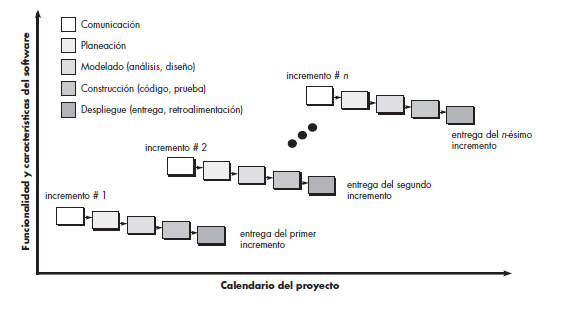
\includegraphics[width=1\textwidth]{Capitulo3/img/ModeloIncremental}
	\caption{Modelo Incremental}
	\label{fig:ModeloIncremental}
\end{figure}

Este tipo de modelo se utilizará debido a que los incrementos nos permiten desarrollar el sistema desde su parte mas fundamental hasta tener el sistema completo y funcionando, obteniendo un entregable en cada uno de los incrementos.
\\
Los incrementos que se realizarán serán los siguientes:
\\
\begin{enumerate}
	\item Se realizará el módulo del sensor el cual consiste en el análisis del sensor de flujo, del microcontrolador a utilizar y la forma de comunicación con la aplicación móvil para el envío del dato de la medición obtenida.
	\item Se hará el diseño y programación para realizar la comunicación entre el sensor y la aplicación y se realizarán las pruebas unitarias pertinentes para asegurar que la medición y comunicación sean correctos.
	\item Se realizará módulo de la aplicación móvil el cual consiste en el análisis y diseño de la aplicación móvil para la obtención de datos, se realizará la programación de la interfaz de la aplicación móvil con la cual el usuario podrá visualizar los datos y se realizaran las pruebas pertinentes.
	\item Se continuará con el análisis, diseño y programación del submódulo de usuarios, en el cual se tendrá una aplicación móvil en la cual el usuario pueda interactuar de una forma fácil y eficiente con el sistema.
	\item Se realizará el análisis, diseño y programación del submódulo para la geolocalización de los establecimientos.
	\item Se realizara el análisis y diseño para el envío y recepción de datos entre la aplicación móvil y el servidor web y se realizarán las pruebas de integración de todo el módulo de la aplicación móvil.
	\item Se realizará el módulo servidor web el cual consiste en el análisis, diseños y programación de la recepción de los datos obtenidos, asimismo se realizarán las pruebas unitarias del incremento en cuestión.
	\item Se continuará con el módulo servidor web con el análisis, diseño y programación para la clasificación de los establecimientos según los resultados obtenidos y se realizarán tanto pruebas unitarias del módulo servidor web..
	\item En este incremento se harán las pruebas de integración del sistema.	
\end{enumerate}


%%%%%%%%%%%%%%%%%%%%%%%%%%%%%%%%%%%%%%%%%%%%%%%%%%%%%%%%%%%%%%%%%%%%%%%%%
%           Capítulo 4: Diseño del Sistema                   %
%%%%%%%%%%%%%%%%%%%%%%%%%%%%%%%%%%%%%%%%%%%%%%%%%%%%%%%%%%%%%%%%%%%%%%%%%

\chapter{Diseño del sistema}\label{chapter4}
\section{Diagrama del proceso general del sistema}
En la Figura \ref{fig:proceso_general} se observa un el diagrama del proceso general del sistema.
\begin{figure}[H]
	\centering
	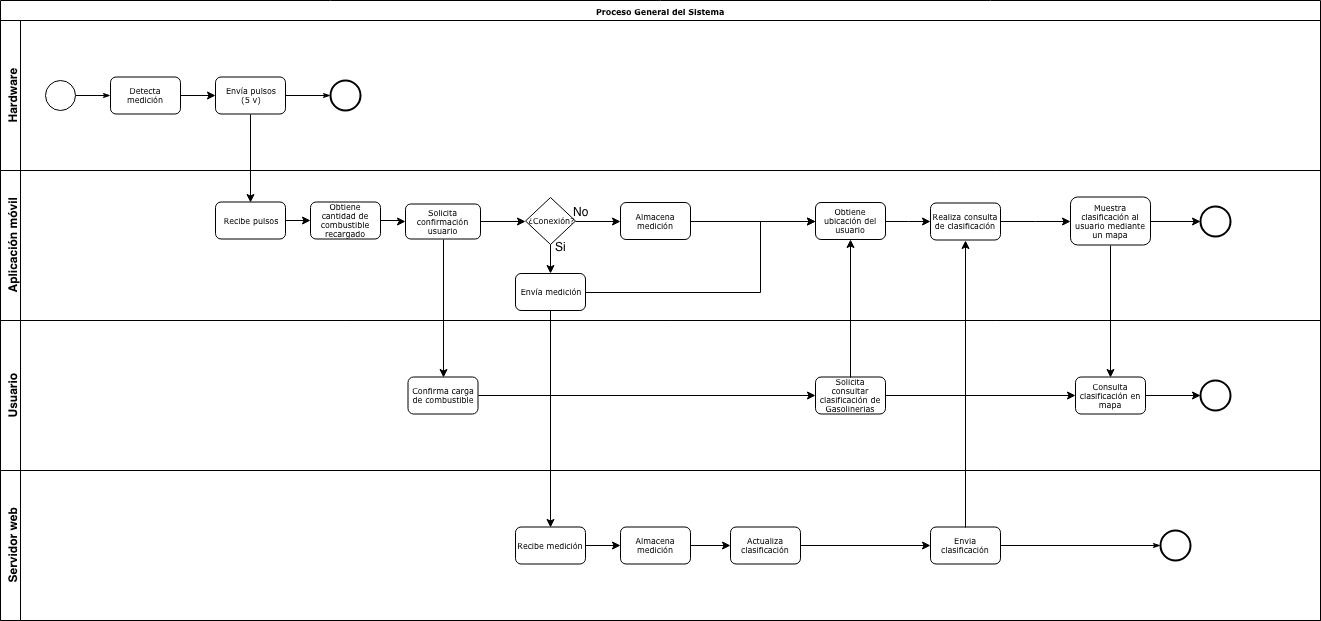
\includegraphics[scale=.35]{Capitulo4/images/proceso_general}
	\caption{Diagrama del proceso general del sistema}
	\label{fig:proceso_general}
\end{figure}
\section{Arquitectura general del sistema}
En la Figura \ref{fig:arquitectura_sistema} se observa un diagrama de la arquitectura general del sistema.
\begin{figure}[H]
	\centering
	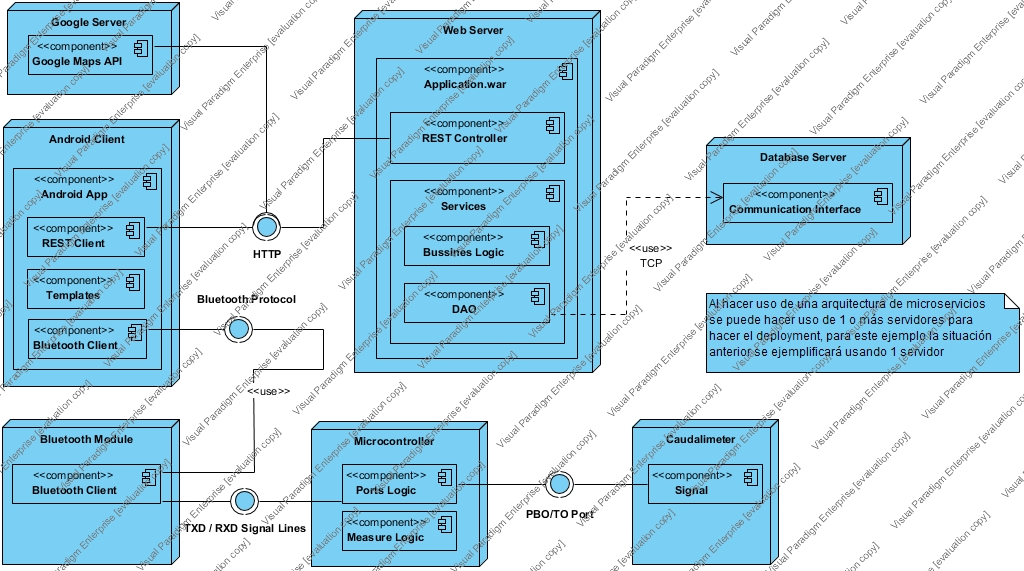
\includegraphics[scale=.44]{Capitulo4/images/arquitectura_sistema}
	\caption{Arquitectura general del sistema}
	\label{fig:arquitectura_sistema}
\end{figure}
\section{Diagrama de clases}
En la Figura \ref{fig:diagrama_clases} se observa el diagrama de clases del sistema.
\begin{figure}[H]
	\centering
	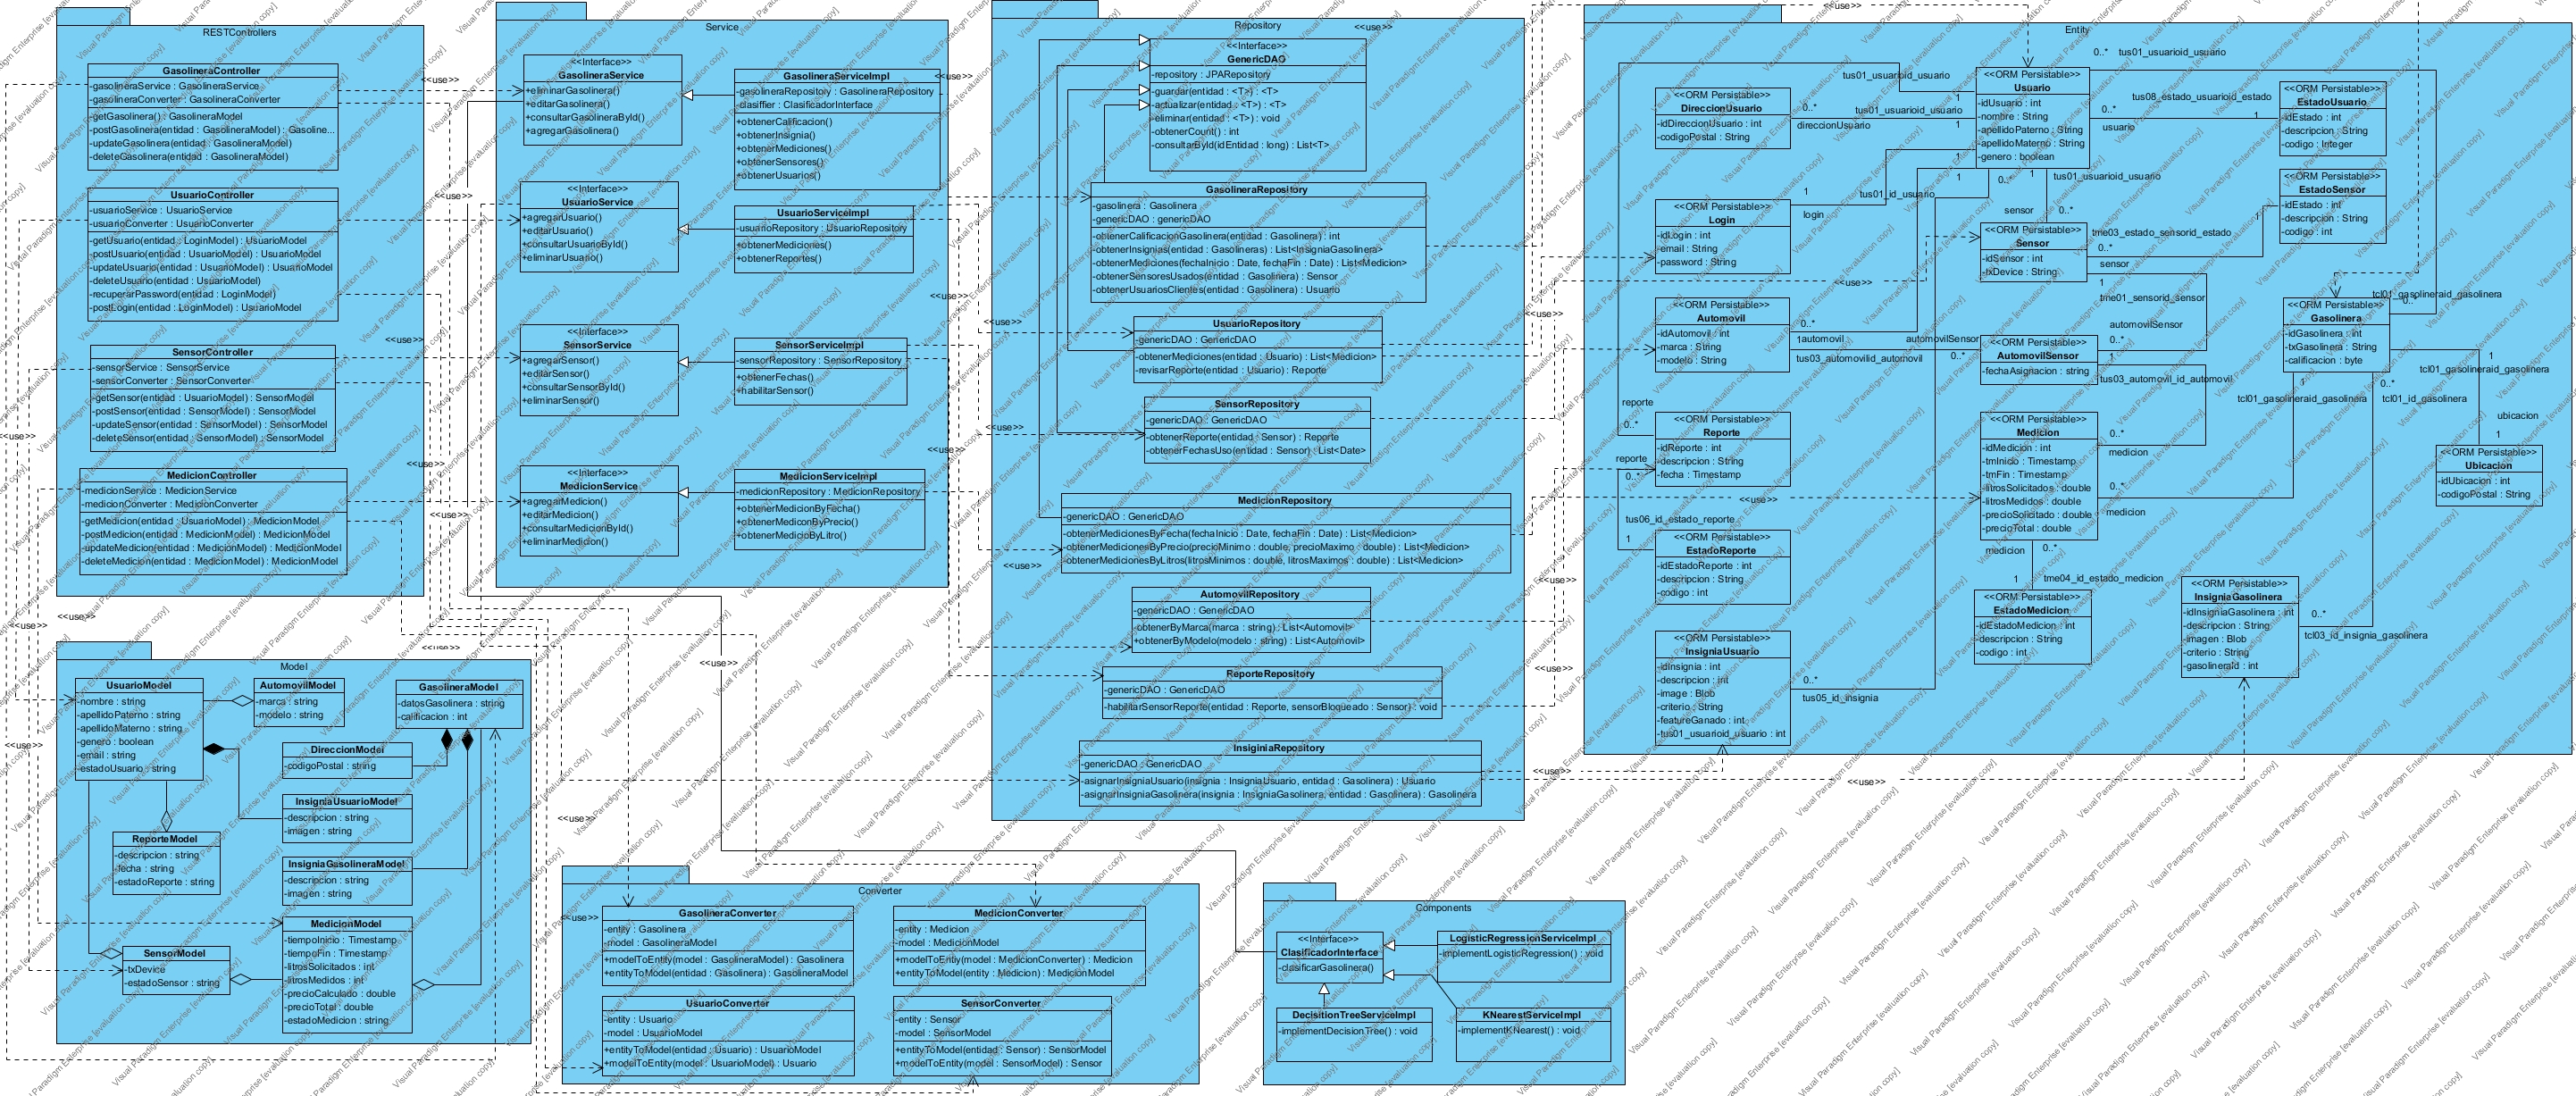
\includegraphics[scale=.21, angle=90]{Capitulo4/images/Clases}
	\caption{Diagrama de clases}
	\label{fig:diagrama_clases}
\end{figure}
\section{Modelo de información del sistema}
En la Figura \ref{fig:modelo_informacion} se observa un diagrama del modelo de información correspondiente al sistema.
\begin{figure}[H]
	\centering
	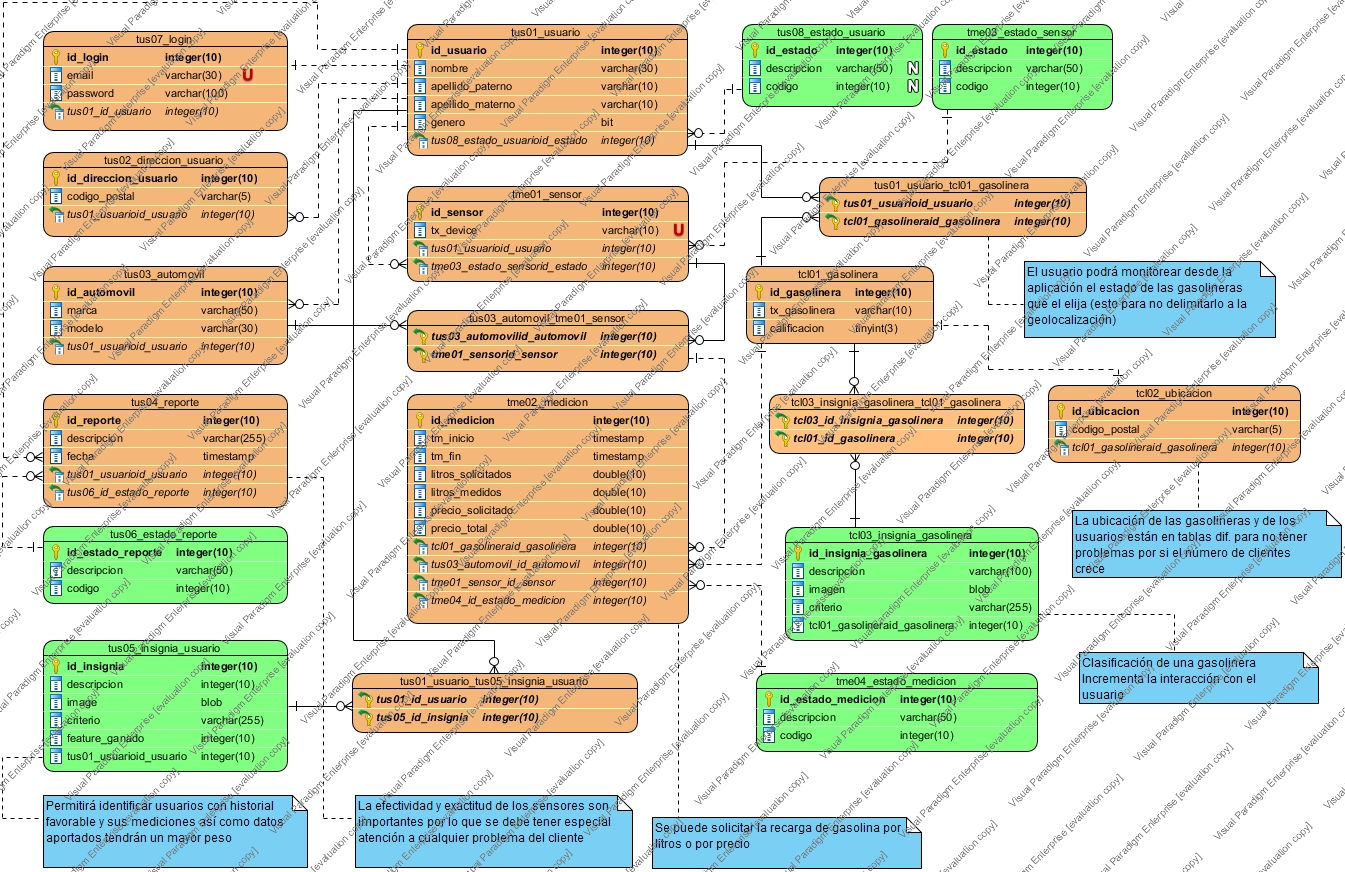
\includegraphics[scale=.34]{Capitulo4/images/modelo_informacion}
	\caption{Modelo de información del sistema}
	\label{fig:modelo_informacion}
\end{figure}
\section{Pruebas de integración}
A continuación se muestran las pruebas de integración de los módulos de hardware y software.
\section{Pruebas de integración}
A continuación se muestran las pruebas de integración de los módulos de hardware y software.
\input{Capitulo6/integracion//Hardware/principal}
\input{Capitulo6/integracion//Software/principal}


\section{Pruebas de integración}
A continuación se muestran las pruebas de integración de los módulos de hardware y software.
\input{Capitulo6/integracion//Hardware/principal}
\input{Capitulo6/integracion//Software/principal}




\section{Pruebas de integración}
A continuación se muestran las pruebas de integración de los módulos de hardware y software.
\section{Pruebas de integración}
A continuación se muestran las pruebas de integración de los módulos de hardware y software.
\input{Capitulo6/integracion//Hardware/principal}
\input{Capitulo6/integracion//Software/principal}


\section{Pruebas de integración}
A continuación se muestran las pruebas de integración de los módulos de hardware y software.
\input{Capitulo6/integracion//Hardware/principal}
\input{Capitulo6/integracion//Software/principal}





%%%%%%%%%%%%%%%%%%%%%%%%%%%%%%%%%%%%%%%%%%%%%%%%%%%%%%%%%%%%%%%%%%%%%%%%%
%           Capítulo 5: Desarrollo del sistema                   %
%%%%%%%%%%%%%%%%%%%%%%%%%%%%%%%%%%%%%%%%%%%%%%%%%%%%%%%%%%%%%%%%%%%%%%%%%

\chapter{Desarrollo del sistema}\label{chapter5}
A continuación, se explica como fue desarrollado el sistema, esto se encuentra dividido en dos secciones; hardware y software.

\section{Pruebas de integración}
A continuación se muestran las pruebas de integración de los módulos de hardware y software.
\section{Pruebas de integración}
A continuación se muestran las pruebas de integración de los módulos de hardware y software.
\input{Capitulo6/integracion//Hardware/principal}
\input{Capitulo6/integracion//Software/principal}


\section{Pruebas de integración}
A continuación se muestran las pruebas de integración de los módulos de hardware y software.
\input{Capitulo6/integracion//Hardware/principal}
\input{Capitulo6/integracion//Software/principal}




\section{Pruebas de integración}
A continuación se muestran las pruebas de integración de los módulos de hardware y software.
\section{Pruebas de integración}
A continuación se muestran las pruebas de integración de los módulos de hardware y software.
\input{Capitulo6/integracion//Hardware/principal}
\input{Capitulo6/integracion//Software/principal}


\section{Pruebas de integración}
A continuación se muestran las pruebas de integración de los módulos de hardware y software.
\input{Capitulo6/integracion//Hardware/principal}
\input{Capitulo6/integracion//Software/principal}





%%%%%%%%%%%%%%%%%%%%%%%%%%%%%%%%%%%%%%%%%%%%%%%%%%%%%%%%%%%%%%%%%%%%%%%%%
%           Capítulo 6: Pruebas del sistema                  %
%%%%%%%%%%%%%%%%%%%%%%%%%%%%%%%%%%%%%%%%%%%%%%%%%%%%%%%%%%%%%%%%%%%%%%%%%

\chapter{Pruebas del sistema}\label{chapter6}
En el presente capítulo, se exponen las diversas pruebas realizadas para verificar y validar el funcionamiento del sistema, tanto de la parte física de hardware como del software (aplicación móvil y servidor).


\section{Pruebas de integración}
A continuación se muestran las pruebas de integración de los módulos de hardware y software.
\section{Pruebas de integración}
A continuación se muestran las pruebas de integración de los módulos de hardware y software.
\input{Capitulo6/integracion//Hardware/principal}
\input{Capitulo6/integracion//Software/principal}


\section{Pruebas de integración}
A continuación se muestran las pruebas de integración de los módulos de hardware y software.
\input{Capitulo6/integracion//Hardware/principal}
\input{Capitulo6/integracion//Software/principal}




\section{Pruebas de integración}
A continuación se muestran las pruebas de integración de los módulos de hardware y software.
\section{Pruebas de integración}
A continuación se muestran las pruebas de integración de los módulos de hardware y software.
\input{Capitulo6/integracion//Hardware/principal}
\input{Capitulo6/integracion//Software/principal}


\section{Pruebas de integración}
A continuación se muestran las pruebas de integración de los módulos de hardware y software.
\input{Capitulo6/integracion//Hardware/principal}
\input{Capitulo6/integracion//Software/principal}




\section{Pruebas de integración}
A continuación se muestran las pruebas de integración de los módulos de hardware y software.
\section{Pruebas de integración}
A continuación se muestran las pruebas de integración de los módulos de hardware y software.
\input{Capitulo6/integracion//Hardware/principal}
\input{Capitulo6/integracion//Software/principal}


\section{Pruebas de integración}
A continuación se muestran las pruebas de integración de los módulos de hardware y software.
\input{Capitulo6/integracion//Hardware/principal}
\input{Capitulo6/integracion//Software/principal}




\section{Pruebas de integración}
A continuación se muestran las pruebas de integración de los módulos de hardware y software.
\section{Pruebas de integración}
A continuación se muestran las pruebas de integración de los módulos de hardware y software.
\input{Capitulo6/integracion//Hardware/principal}
\input{Capitulo6/integracion//Software/principal}


\section{Pruebas de integración}
A continuación se muestran las pruebas de integración de los módulos de hardware y software.
\input{Capitulo6/integracion//Hardware/principal}
\input{Capitulo6/integracion//Software/principal}




%%%%%%%%%%%%%%%%%%%%%%%%%%%%%%%%%%%%%%%%%%%%%%%%%%%%%%%%%%%%%%%%%%%%%%%%%
%           Capítulo 7: Conclusiones                  %
%%%%%%%%%%%%%%%%%%%%%%%%%%%%%%%%%%%%%%%%%%%%%%%%%%%%%%%%%%%%%%%%%%%%%%%%%
\chapter{Conclusiones}\label{chapter7}
La problemática planteada explicas las fallas existentes en el despacho de gasolina, esta es una problemática real que afecta a una gran cantidad de automovilistas (como lo muestran las encuestas realizadas) los cuales no cuentan con las herramientas necesarias para saber, que gasolineras presentan estás fallas y cuales no. 

El presente trabajo terminal, permite a los automovilistas de la CDMX conocer que gasolineras presentan irregularidades en los litros despachado, con lo cual, dichos automovilistas podrán tomar una decisión informada sobre donde cargar gasolina.

Como se ha presentado en los capítulos anteriores, el trabajo terminal es factible en cada uno de los ámbitos, tanto técnico, como operativo, y económico. Además de que este usa tecnología robusta y de vanguardia para así brindar el mejor servicio a los posibles usuarios. Bajo una arquitectura flexible y robusta como la de microservicios y usando una lenguaje de programación que es estándar en el mercado como Java, el trabajo terminal cuenta con todas las características suficientes para satisfacer los requerimientos funcionales establecidos, y por ende, el objetivo del trabajo terminal.

Del lado del cliente, se realizó una aplicación Android que permite la Geolocalización del usuario, la interacción con su sensor, el manejo de sus datos y la búsqueda de gasolineras a su alrededor. Dicha aplicación se conecta de forma exitosa a nuestro servidor el cual es capaz de almacenar los datos y realizar la clasficiaciones de gasolineras necesarias. De igual forma se desarrollo un prototipo de sensor el cuál permite conocer la cantidad de litros ingresados a un automóvil con un error del 3.9 por ciento, lo cuaĺ esta dentro del rango permitido por la Normas mexicanas para instrumentos de medición.

De esta forma podemos decir que el proyecto terminal cumple con sus objetivos tanto general como específicos brindando a los usuarios finales un "Prototipo de aplicación Móvil para el reporte y medición de la cantidad de combustible que se suministra a un automóvil como el mismo nombre de nuestro TT así lo expresa.



\chapter{Trabajo futuro}\label{chapter8}
Mejorar el diseño del sensor basado en la norma mexicana NOM-001-SCFI-1993, para asegurar la seguridad, de los usuarios, al momento de utilizar el sistema en el automóvil, así como reducir el tamaño del sensor y del circuito integrado al llevarlo a un ambiente productivo.
\\
Asimismo para tener un mejor resultado con respecto a la medición se utilizará un apego a la norma mexicana NOM-005-SCFI-2011 la cual se refiere al uso de instrumentos y sistemas para la medición de gasolina y otros combustibles líquidos,la cual brinda la aprobación del método de medición así como de una correcta verificación del flujo de combustible, y a su vez buscar tener una certificación de medición del sensor por parte del Centro Nacional de Metrología (CENAM).
\\
Como parte final, la información recabada por los usuarios del sistema puede ser utilizada para generar estadísticas especificas relacionada a la carga de combustible y de esta manera conocer como se comporta la Ciudad de México en el ámbito de carga de combustible.
\chapter{Glosario}\label{chapter9}
\noindent \textbf{API} Es un conjunto de reglas (código) y especificaciones que las aplicaciones pueden seguir para comunicarse entre ellas \citep{API}
\\
\textbf{Caracterización} Calcular por medio de medidas lo mas exactas posibles la ecuación característica del comportamiento del mismo, siendo esta la que determina la razón de cambio de la variable de salida respecto a la de entrada \cite{CARA}
\\
\textbf{Caudalímetro} Un caudalímetro es un instrumento de medida para la medición de caudal o gasto volumétrico de un fluido \citep{MarcoTeorico10}
\\
\textbf{Gateway} es un dispositivo, con frecuencia un ordenador, que permite interconectar redes con protocolos y arquitecturas diferentes a todos los niveles de comunicación. Su propósito es traducir la información del protocolo utilizado en una red al protocolo usado en la red de destino \cite{GATE}
\\
\textbf{Geolocalización} ULa tecnología del geoetiquetado se basa en la información posicional proporcionada por el sistema del sistema de posicionamiento global (GPS), y se transfiere como metadatos a los archivos que sean compatibles con este tipo de información \citep{GEO}
\\
\textbf{Interfaz} Dispositivo capaz de transformar las señales generadas por un aparato en señales comprensibles por otro.\citep{INTERFAZ}
\\
\textbf{Microservicios} Los microservicios son tanto un estilo de arquitectura como un modo de programar software. Con los microservicios, las aplicaciones se dividen en sus componentes más pequeños e independientes entre sí. \citep{MICROSERVICIOS}
\\
\textbf{Módulo} Es una porción de un programa de ordenador. \citep{MODULO}
\\
\textbf{Protocolo} Es un reglamento o una serie de instrucciones que se fijan por tradición o por convenio \citep{PROTOCOLO}
\\
\textbf{Requerimiento} Atributo necesario dentro de un sistema, que puede representar una capacidad, una característica o un factor de calidad del sistema \citep{REQUERIMIENTO}
\\
\textbf{Software} Soporte lógico de un sistema informático, que comprende el conjunto de los componentes lógicos necesarios que hacen posible la realización de tareas específicas\citep{SOFTWARE}





%%%%%%%%%%%%%%%%%%%%%%%%%%%%%%%%%%%%%%%%%%%%%%%%%%%%%
%                   APÉNDICES                       %
%%%%%%%%%%%%%%%%%%%%%%%%%%%%%%%%%%%%%%%%%%%%%%%%%%%%%
\appendix
% this file is called up by thesis.tex
% content in this file will be fed into the main document
\chapter{Anexos}
% top level followed by section, subsection

% \section{Apéndice}


%\section{Manual de usuario}
Aquí va el manual de usuario
\section{Cronogramas de actividades}
\subsection{Castillo Reyes Juan Daniel}
El cronograma del alumno se muestra en la Figura \ref{fig:cronograma_batiz}.
\begin{figure}[H]
	\centering
	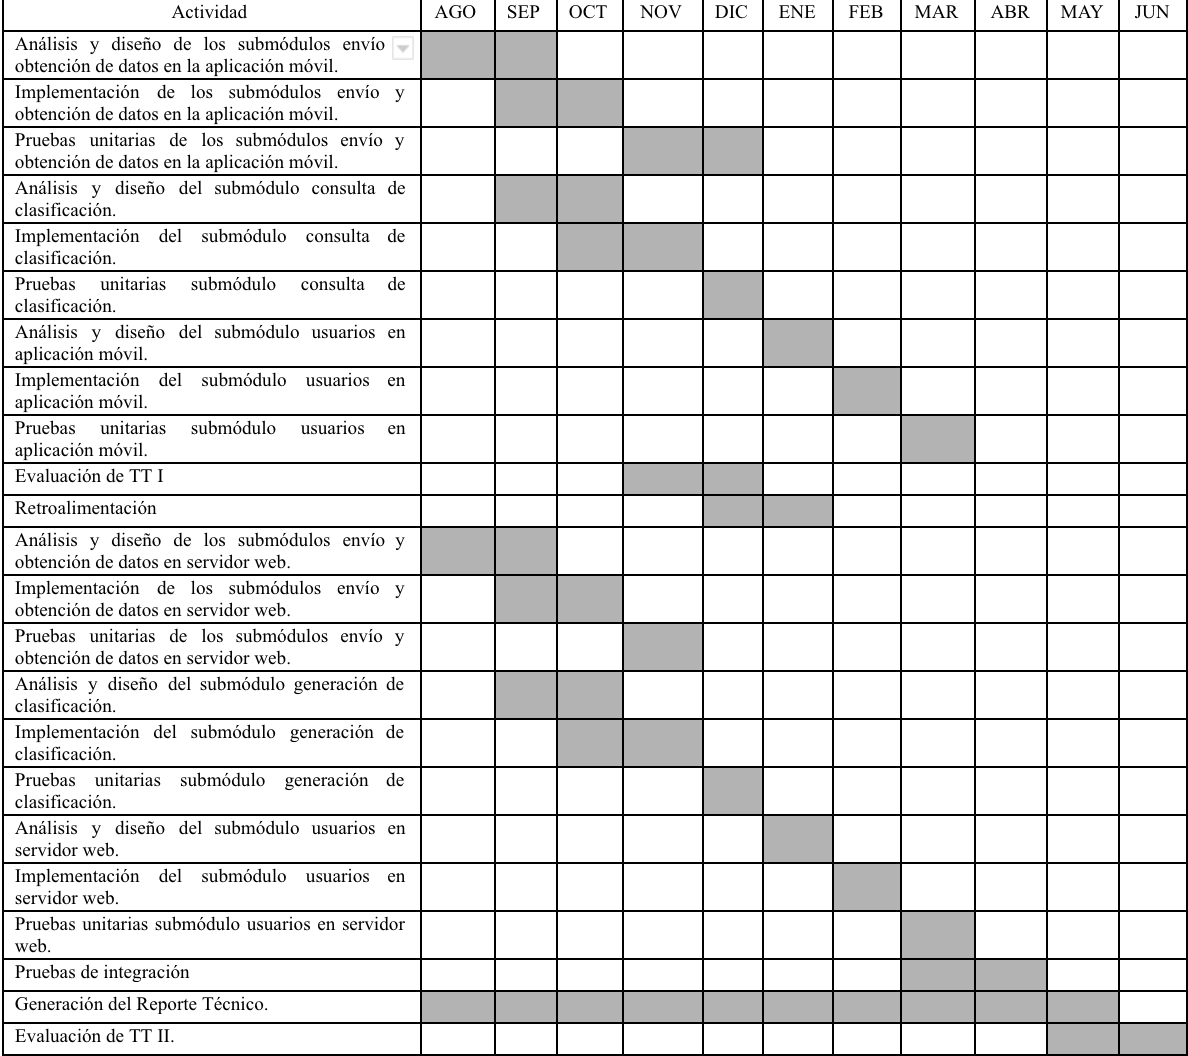
\includegraphics[width=1\textwidth]{Apendice1/cronogramas/batiz}
	\caption{Cronograma de Castillo Reyes Juan Daniel}
	\label{fig:cronograma_batiz}
\end{figure}
\subsection{Monroy Martos Elioth}
El cronograma del alumno se muestra en la Figura \ref{fig:cronograma_elioth}.
\begin{figure}[H]
	\centering
	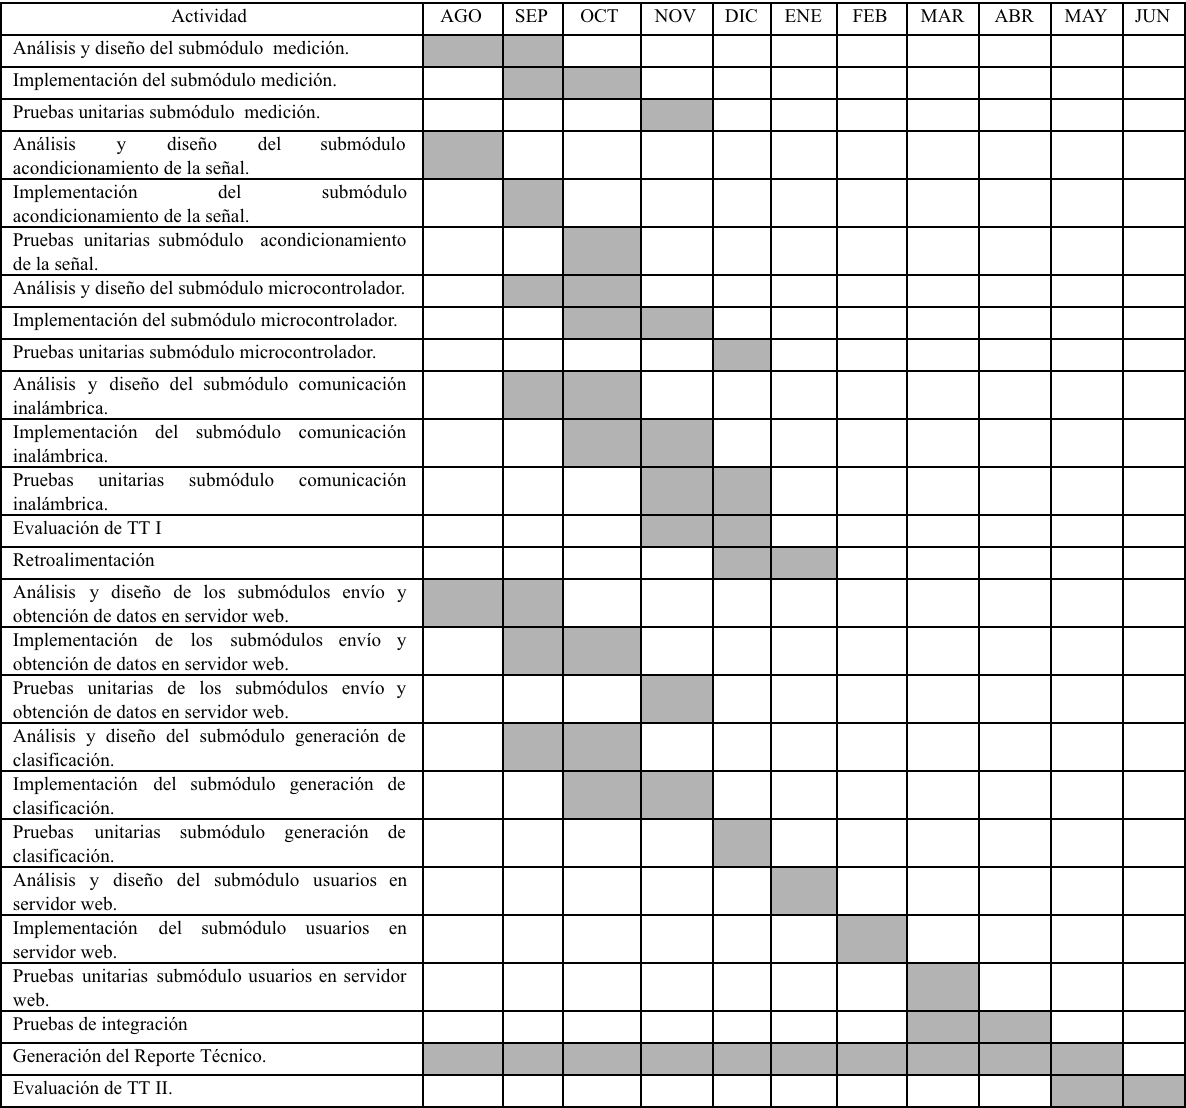
\includegraphics[width=1\textwidth]{Apendice1/cronogramas/elioth}
	\caption{Cronograma de Monroy Martos Elioth}
	\label{fig:cronograma_elioth}
\end{figure}
\subsection{Naranjo Miranda Javier Said}
El cronograma del alumno se muestra en la Figura \ref{fig:cronograma_said}.
\begin{figure}[H]
	\centering
	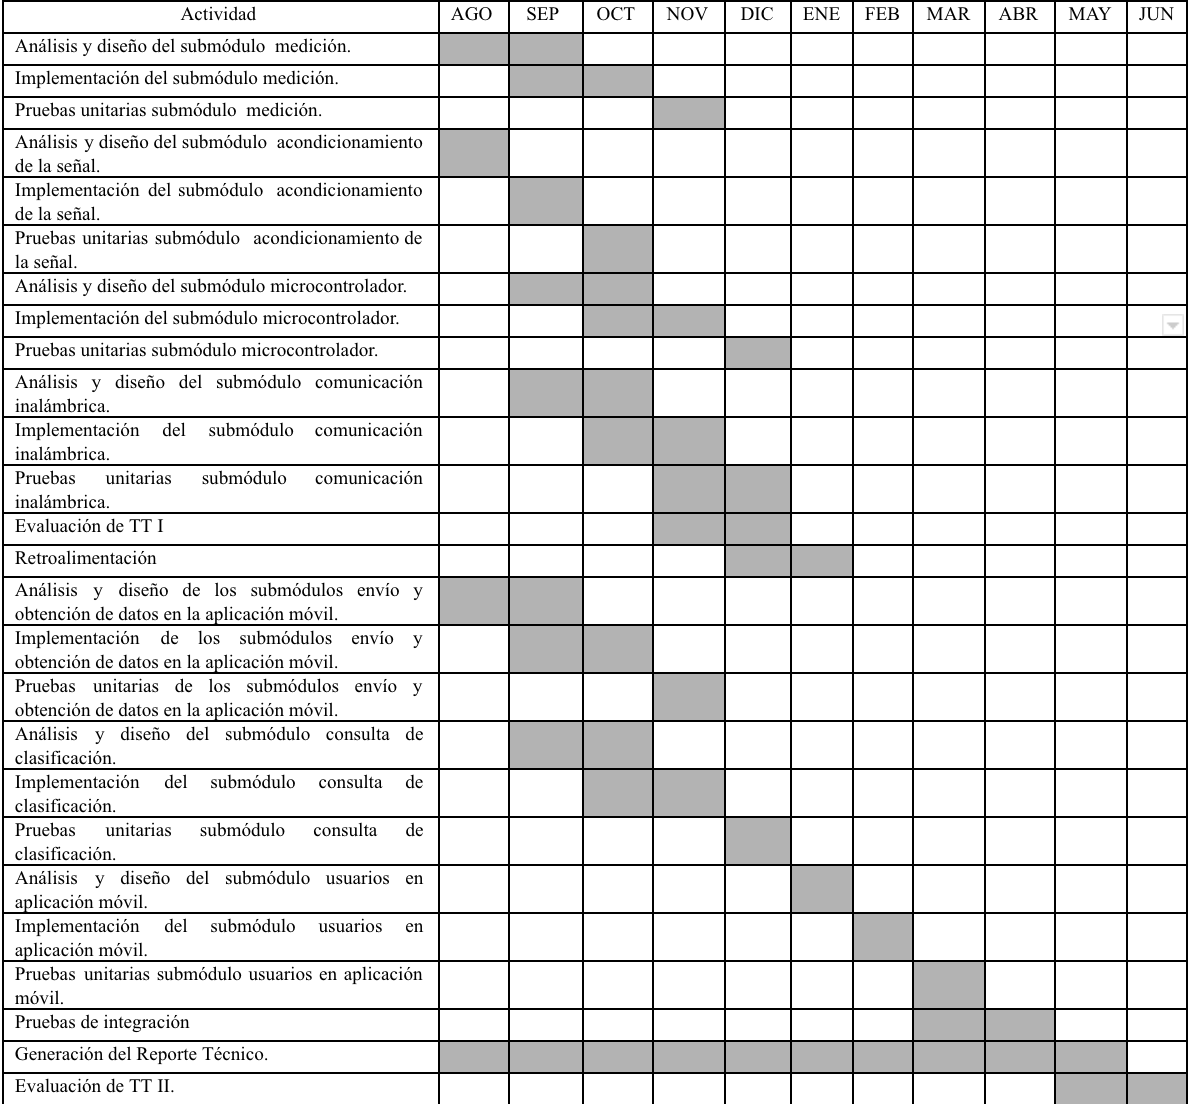
\includegraphics[width=1\textwidth]{Apendice1/cronogramas/said}
	\caption{Cronograma de Naranjo Miranda Javier Said}
	\label{fig:cronograma_said}
\end{figure}
\section{Cambios en los cronogramas de actividades}
A continuación, se presentan los cambios realizados en el cronograma entregado durante el inicio del Trabajo Terminal (protocolo). Las subsiguientes secciones se dividen en cada uno de los integrantes del trabajo y las correcciones que hubo en sus cronogramas.
\subsection{Castillo Reyes Juan Daniel}
\begin{itemize}
	\item La actividad \textit{Pruebas unitarias y submódulo comunicación inalámbrica} fue eliminada debido a que está actividad fue designada a \textit{Monroy Martos Elioth} y \textit{Naranjo Miranda Javier Said}. Permitiendo así que, \textit{Castillo Reyes Juan Daniel} pudiera enfocarse a otras actividades relacionadas mayormente con el desarrollo del servidor web y la aplicación móvil.
	\item La actividad \textit{Evaluación de TT I} fue reacomodada para una mejor lectura del cronograma.
	\item La actividad \textit{Retroalimentación} fue añadida debido a los posibles cambios que pueden ser señalados por los Profesores Sinodales después de la Presentación de Trabajo Terminal I.
\end{itemize}
\subsection{Monroy Martos Elioth}
\begin{itemize}
	\item La actividad \textit{Retroalimentación} fue añadida debido a los posibles cambios que pueden ser señalados por los Profesores Sinodales después de la presentación de Trabajo Terminal I.
	\item Las actividades \textit{Análisis y diseño del submódulo acondicionamiento de la señal}, \textit{Implementación del submódulo acondicionamiento de la señal} y \textit{Pruebas unitarias submódulo acondicionamiento de la señal} fueron eliminadas debido a que el sensor y el microcontrolador seleccionados para la realización del Trabajo Terminal no requieren de un acondicionamiento de la señal (véanse las secciones \ref{sec:Sensor} y \ref{sec:micro}). Esto debido a que el voltaje que arroja el sensor es menor a 5 volts y el microcontrolador soporta como entrada el voltaje que manda el sensor.
\end{itemize}
\subsection{Naranjo Miranda Javier Said}
\begin{itemize}
	\item Las fechas de la actividades \textit{Análisis y diseño del submódulo medición}, \textit{Implementación del submódulo medición}, \textit{Pruebas unitarias submódulo medición}, \textit{Análisis y diseño del submódulo microcontrolador}, \textit{Implementación del submódulo microcontrolador}, \textit{Pruebas unitarias submódulo microcontrolador}, \textit{Análisis y diseño del submódulo comunicación inalámbrica}, \textit{Implementación del submódulo comunicación inalámbrica} y \textit{Pruebas unitarias del submódulo comunicación inalámbrica} fueron corregidas debido a que se encontraban en desorden, en general las fechas de las actividades fueron desplazadas una fila hacía arriba.
	\item La actividad \textit{Retroalimentación} fue añadida debido a los posibles cambios que pueden ser señalados por los Profesores Sinodales después de la presentación de Trabajo Terminal I.
	\item Las actividades \textit{Análisis y diseño del submódulo acondicionamiento de la señal}, \textit{Implementación del submódulo acondicionamiento de la señal} y \textit{Pruebas unitarias submódulo acondicionamiento de la señal} fueron eliminadas debido a que el sensor y el microcontrolador seleccionados para la realización del Trabajo Terminal no requieren de un acondicionamiento de la señal (véanse las secciones \ref{sec:Sensor} y \ref{sec:micro}). Esto debido a que el voltaje que arroja el sensor es menor a 5 volts y el microcontrolador soporta como entrada el voltaje que manda el sensor.
\end{itemize}
\section{Atraso en las actividades de los cronogramas}\label{anexo:atraso}
Durante la realización del presente trabajo, se sufrió un atraso en algunas de las actividades marcadas en los cronogramas. Las actividades afectadas fueron:
\begin{itemize}
	\item \textit{Análisis y diseño de los submódulos envío y obtención de datos en servidor web}: Atraso de 3 semanas debido a que al momento de establecer la arquitectura del sistema (microservicios), fue necesario realizar una investigación sobre las posibles arquitecturas y posteriormente aprender sobre la arquitectura seleccionada, lo cual impedía que se pudiera realizar un diseño y análisis de este módulo, al igual que causó un atraso en las actividades relacionadas con el servidor web como: \textit{Implementación de los submódulos envío y obtención de datos en servidor web}, \textit{Pruebas unitarias de los submódulos envío y obtención de datos en servidor web}, \textit{Análisis y diseño del submódulo consulta de clasificación}, \textit{Implementación del submódulo consulta de clasificación}, \textit{Pruebas unitarias submódulo consulta de clasificación}, \textit{Análisis y diseño del submódulo usuarios en aplicación móvil}, \textit{Implementación del submódulo usuarios en aplicación móvil}, \textit{Pruebas unitarias del submódulo usuarios en aplicación móvil}, \textit{Análisis y diseño del submódulo usuarios en servidor web}, \textit{Implementación del submódulo usuarios en servidor web}, \textit{Pruebas unitarias del submódulo usuarios en servidor web}.
	\item Las actividades \textit{Implementación del submódulo medición}, \textit{Pruebas unitarias submódulo medición}, \textit{Implementación del submódulo microcontrolador}, \textit{Pruebas unitarias submódulo microcontrolador}, \textit{Implementación del submódulo comunicación inalámbrica}, \textit{Pruebas unitarias submódulo comunicación inalámbrica} sufrieron un atraso de un mes, debido a que el sensor de flujo a usar, tardo un mes más en llegar de lo esperado.
\end{itemize}
\section{Encuesta} \label{FactibilidadOperativa}
\textbf{Gasolimetro}
\\Se lanzará al mercado una aplicación móvil que permite conocer las gasolineras que cargan con mayor exactitud el combustible solicitado por el usuario. El sistema consta de un sensor que permite medir el flujo de gasolina introducido en el vehículo.
La siguiente encuesta nos ayudará a medir los niveles de aceptación del producto. La información proporcionada solo se utilizara para fines estadísticos.
\\
\begin{enumerate}
	\item Edad: \\ a.-16 a 20 años\hspace{1cm}b.-21 a 30 años\hspace{1cm}c.-31 a 40 años\hspace{1cm}d.-mas de 40 años
	\item Delegación: \rule{20mm}{0.1mm}
	\item Ocupación:\\ a.-Estudiante\hspace{1cm}b.-Profesionista\hspace{1cm}c.-Empleado\hspace{1cm}d.-Independiente
	\item ¿Con qué tipo de automóvil cuenta?\\ a.-De combustión\hspace{1cm}b.-Híbrido\hspace{1cm}c.-Eléctrico\hspace{1cm}d.-No tengo auto
	\item ¿Qué tan seguido carga gasolina?:\\ a.-más de 3 veces por semana\hspace{1cm}b.-2 o 3 veces por semana\hspace{1cm}c.-1 vez a la semana\hspace{1cm}d.-No cargo gasolina
	\item En promedio ¿Cuánto carga de gasolina?(En pesos)\\más de \$500 \hspace{1cm}b.-Entre \$300 y \$500\hspace{1cm}c.-Entre \$100 y \$300 \hspace{1cm}d.-menos de \$100
	\item Del 1 al 5, donde 1 es poco y 5 es mucho ¿Con qué precisión considera que le cargan litros completos? \rule{20mm}{0.1mm}
	\item ¿Actualmente utiliza algún medio para medir los litros que le cargan?\\ a.-Si\hspace{1cm}b.-No
	\item Pensando en la descripción del producto y en los beneficios que este ofrece ¿Qué tan interesante le parece el producto?
	\\ a.-Muy interesante\hspace{1cm}b.-Interesante\hspace{1cm}c.-Poco interesante\hspace{1cm}d.-No me interesa
	\item ¿Cuánto considera que es un precio adecuado para su venta?
	\\ a.-menos de \$300 \hspace{1cm}b.-Entre \$300 y \$500 \hspace{1cm}c.-Entre \$500 y \$800 \hspace{1cm}d.-mas de \$800
	\item ¿En qué sistema operativo le gustaría que este producto estuviera a la venta?\\ a.-Android\hspace{1cm}b.-IOS\hspace{1cm}c.-Windows Phone
	\item ¿Qué tan útil le resulta este producto?\\ a.-Muy útil\hspace{1cm}b.-Útil\hspace{1cm}c.-Poco útil\hspace{1cm}d.-Nada útil
	\item En una escala del 1 al 5, donde 1 es poco y 5 es mucho ¿Qué probabilidad hay de que consuma este producto?\rule{20mm}{0.1mm}
\end{enumerate}
\section{Resultados de la encuesta}
A continuación se muestran los resultados de la encuesta.
\begin{figure}[H]
		\centering
		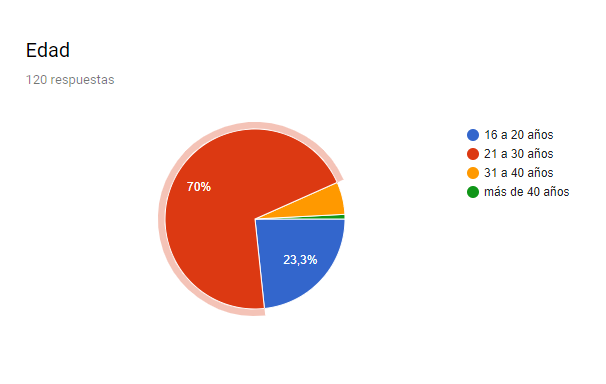
\includegraphics[width=0.5\textwidth]{Apendice2/img/Edad}
		\caption{Resultado pregunta 1}
	\end{figure}
 \begin{figure}[H]
	\centering
	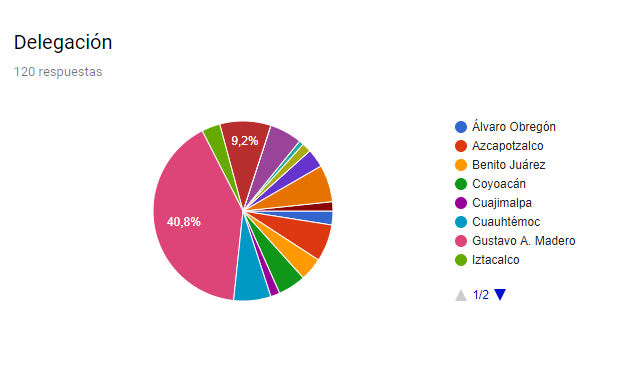
\includegraphics[width=0.5\textwidth]{Apendice2/img/Delegacion}
	\caption{Resultado pregunta 2}
\end{figure}
 \begin{figure}[H]
		\centering
		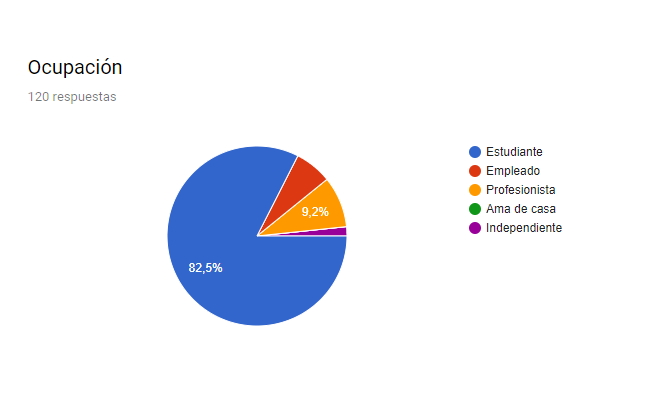
\includegraphics[width=0.5\textwidth]{Apendice2/img/Ocupacion}
		\caption{Resultado pregunta 3}
	\end{figure}
\begin{figure}[H]
	\centering
	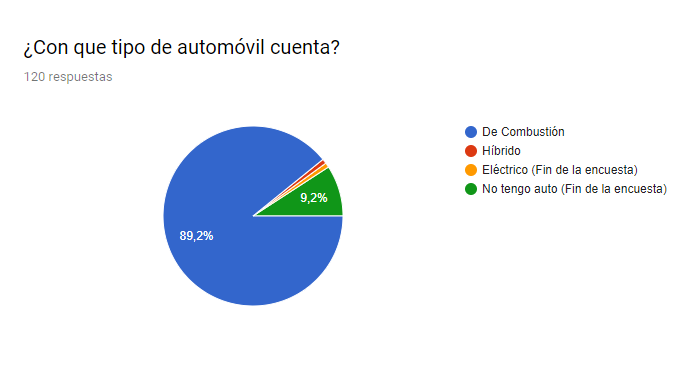
\includegraphics[width=0.5\textwidth]{Apendice2/img/TipoAutomovil}
	\caption{Resultado pregunta 4}
\end{figure}
\begin{figure}[H]
	\centering
	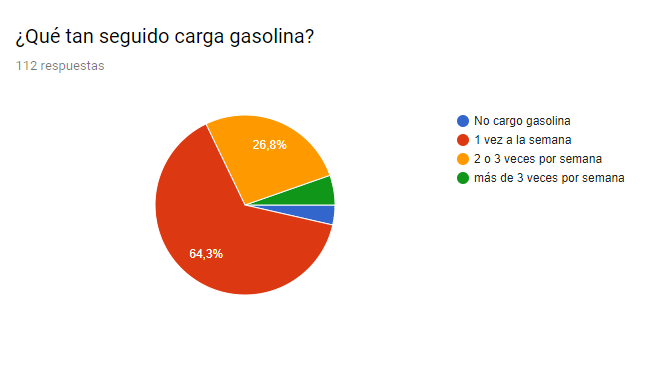
\includegraphics[width=0.5\textwidth]{Apendice2/img/FrecuenciaGasolina}
	\caption{Resultado pregunta 5}
\end{figure}
\begin{figure}[H]
	\centering
	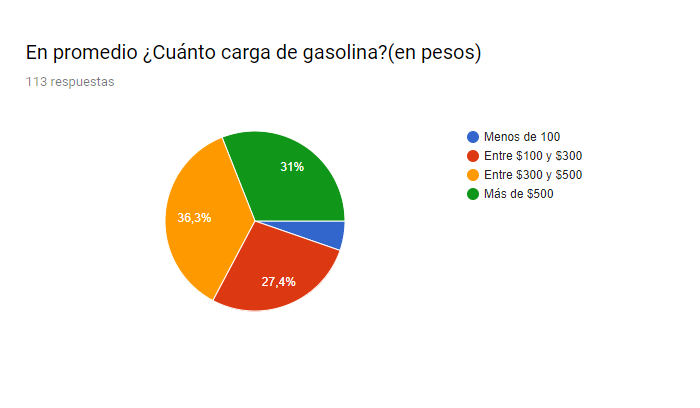
\includegraphics[width=0.5\textwidth]{Apendice2/img/CargaGasolina}
	\caption{Resultado pregunta 6}
\end{figure}
\begin{figure}[H]
	\centering
	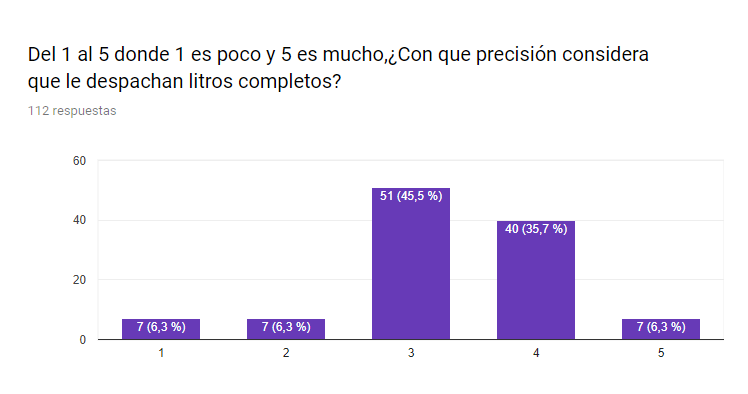
\includegraphics[width=0.5\textwidth]{Apendice2/img/Precision}
	\caption{Resultado pregunta 7}
\end{figure}
\begin{figure}[H]
	\centering
	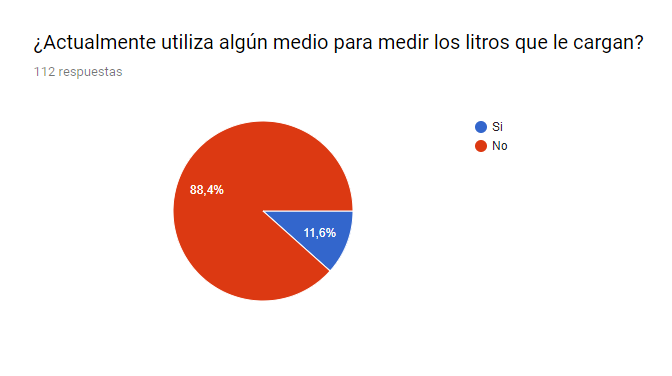
\includegraphics[width=0.5\textwidth]{Apendice2/img/Metodo}
	\caption{Resultado pregunta 8}
\end{figure}
\begin{figure}[H]
	\centering
	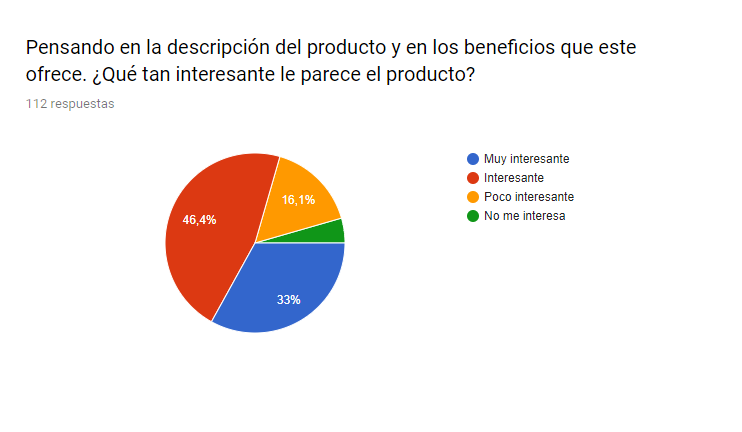
\includegraphics[width=0.5\textwidth]{Apendice2/img/Interesante}
	\caption{Resultado pregunta 9}
\end{figure}
\begin{figure}[H]
	\centering
	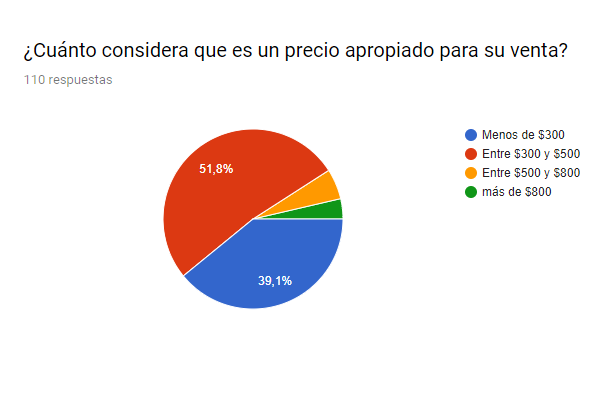
\includegraphics[width=0.5\textwidth]{Apendice2/img/Precio}
	\caption{Resultado pregunta 10}
\end{figure}
\begin{figure}[H]
	\centering
	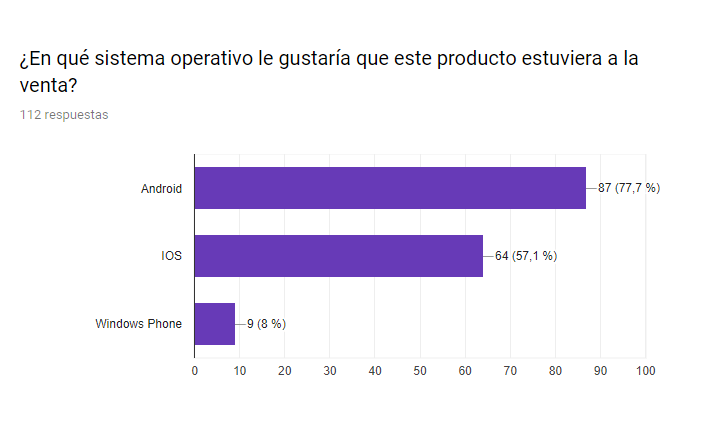
\includegraphics[width=0.5\textwidth]{Apendice2/img/SO}
	\caption{Resultado pregunta 11}
\end{figure}
\begin{figure}[H]
	\centering
	%\includegraphics[width=0.5\textwidth]{Apendice2/img/Util}
	\caption{Resultado pregunta 12}
\end{figure}
\begin{figure}[H]
	\centering
	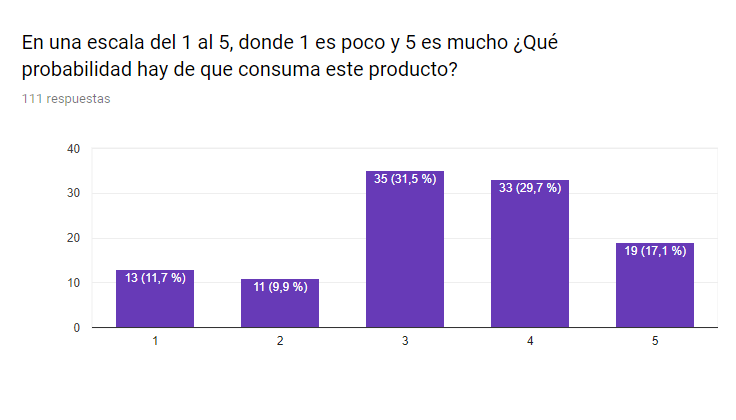
\includegraphics[width=0.5\textwidth]{Apendice2/img/Consumir}
	\caption{Resultado pregunta 13}
\end{figure} 

               % Colocar los circuitos, manuales, código fuente, pruebas de teoremas, etc.
%%%%%%%%%%%%%%%%%%%%%%%%%%%%%%%%%%%%%%%%%%%%%%%%%%%%%
%                   REFERENCIAS                     %
%%%%%%%%%%%%%%%%%%%%%%%%%%%%%%%%%%%%%%%%%%%%%%%%%%%%%
% existen varios estilos de bilbiografía, pueden cambiarlos a placer
\bibliographystyle{ieeetr} % otros estilos pueden ser abbrv, acm, alpha, apalike, ieeetr, plain, siam, unsrt

%El formato trae otros estilos, o pueden agregar uno que les guste:
%\bibliographystyle{Latex/Classes/PhDbiblio-case} % title forced lower case
%\bibliographystyle{Latex/Classes/PhDbiblio-bold} % title as in bibtex but bold
%\bibliographystyle{Latex/Classes/PhDbiblio-url} % bold + www link if provided
%\bibliographystyle{Latex/Classes/jmb} % calls style file jmb.bst

\bibliography{Bibliografia/referencias}             % Archivo .bib


\end{document}
